\pdfoutput=1
\pdfcompresslevel=9
\pdfinfo
{
  /Author ()
  /Title ()
  /Subject ()
  /Keywords ()
}
\documentclass[a4paper,onecolumn,twoside,12pt]{mwrep}
\newcommand{\norm}[1]{\left\lVert#1\right\rVert}
\usepackage{enumitem}
\usepackage{times}
\usepackage[utf8x]{inputenc}
\usepackage[T1]{fontenc}
\usepackage{bbm}
\usepackage{placeins}
\usepackage{graphicx}
\usepackage{epstopdf}
\usepackage[numbers]{natbib}
\usepackage{lineno,hyperref}
\usepackage{float}
\usepackage{subfigure}
\modulolinenumbers[5]
\usepackage{amsfonts,amssymb,graphicx,color}
\usepackage[]{algorithm2e}
\newcommand\scalemath[2]{\scalebox{#1}{\mbox{\ensuremath{\displaystyle #2}}}}
\usepackage{amsmath}
\DeclareMathOperator{\sgn}{sgn}
\hyphenpenalty=10000		% nie dziel wyrazów zbyt często
\clubpenalty=10000			% kara za sierotki
\widowpenalty=10000			% nie pozostawiaj wdów
\brokenpenalty=10000		% nie dziel wyrazów między stronami
\exhyphenpenalty=999999		% nie dziel słów z myślnikiem
\righthyphenmin=3			% dziel minimum 3 litery
\usepackage{amsthm}
\tolerance=4500
\pretolerance=250
\hfuzz=1.5pt
\hbadness=1450
\sloppy						% umacnia pozycję prawego marginesu

\setlength{\textwidth}{\paperwidth}
\addtolength{\textwidth}{-5cm}
\setlength{\textheight}{\paperheight}
\addtolength{\textheight}{-5cm}
\setlength{\oddsidemargin}{1cm}
\setlength{\evensidemargin}{0cm}
\topmargin -1.25cm
\footskip 1.4cm

\usepackage{geometry}
\geometry{lmargin=3cm,rmargin=2cm}


\linespread{1.3}

\def\code#1{\texttt{#1}}
\DeclareMathOperator*{\argmaxB}{argmax}
\setcounter{secnumdepth}{3}
\begin{document}

\theoremstyle{plain}
\newtheorem{defn}{Definition}[chapter]
\newtheorem{prop}{Property}[chapter]
\newtheorem{exmp}{Example}[section]

\begin{titlepage}
	\begin{center}
	\fontsize{20pt}{34pt}\selectfont
	Wrocław University of~Science and Technology \\
	\vspace*{.6\baselineskip}
	\fontsize{20pt}{18pt}\selectfont
	Faculty of~Geoengineering, Mining and Geology

	\vspace*{4\baselineskip}
	
	\fontsize{20pt}{15pt}\selectfont
	mgr inż. Jacek Wodecki\\%
	\vspace*{3.15\baselineskip}
	\fontseries{b}\fontsize{20pt}{18pt}\selectfont
	Methods of~multidimensional data processing \\for damage detection in~mining machines \\
		\vspace*{1.15\baselineskip}
	\fontseries{b}\fontsize{20pt}{18pt}\selectfont
  Metody przetwarzania danych wielowymiarowych w~detekcji uszkodzeń maszyn górniczych \\
	\vspace*{2.15\baselineskip}
	\fontseries{m}\fontsize{20pt}{20pt}\selectfont
	Doctoral Dissertation \\
	
	\end{center}
	\vspace*{3.15\baselineskip}
		\begin{flushright}
	\fontseries{m}\fontsize{16pt}{16pt}\selectfont
Thesis advisor\\
	dr hab. inż. Radosław Zimroz, prof. uczelni\\
	\end{flushright}
		\vspace*{1\baselineskip}
		\begin{center}
	\fontseries{m}\fontsize{14pt}{1pt}\selectfont
	Wrocław 2019
  \end{center}
  

% \clearpage \newpage \mbox{~} \clearpage \newpage
\cleardoublepage
\thispagestyle{empty}
\end{titlepage}
% \vspace*{2\baselineskip}


\begin{flushright}

% \textit{"Problems worthy of~attack prove their worth by~fighting back."\\
% - Piet Hein}

\textit{"The Universe is~under no obligation to~make sense to~you."\\
- dr Neil deGrasse Tyson}
\end{flushright}

\vspace*{21\baselineskip}

\begin{center}
	\textit{
\textbf{Autor pracy pragnie podziękować}}
\end{center}

\begin{flushleft}
% \textit{Autor pracy pragnie podziękować:} \\ 
\vspace*{1\baselineskip}
\textit{Żonie, za nieustanne wsparcie i motywację.} \\
\vspace*{1\baselineskip}
\textit{Promotorowi, za cenne uwagi i cierpliwość w trakcie trwania studiów doktoranckich.} \\
\vspace*{1\baselineskip}
\textit{Współpracownikom, za wszelką pomoc i wsparcie.} \\


\end{flushleft}

% \vspace*{12\baselineskip}


% \clearpage \newpage \mbox{~} \clearpage \newpage
\cleardoublepage
\thispagestyle{empty}
\newpage

% streszczenie
\begin{center}
\textbf{Streszczenie}
\end{center}

W związku z~postępującą automatyzacją procesów we~wszyskich gałęziach gospodarki, współczesny przemysł wydobywczy wykazuje wysokie zapotrzebowanie na~zdalne wykrywanie uszkodzeń maszyn górniczych w sposób automatyczny. Ciągła poprawa wydajności i~dokładności algorytmów analitycznych pozwala na wykrywanie wczesnych form uszkodzeń celem zapobiegania awariom, oraz świadome planowanie inspekcji i~napraw. W~przypadku analizy sygnałów rzeczywistych zarejestrowanch w czasie pracy maszyn, konieczne jest uwzględnienie różnego rodzaju składowch (zarówno losowch jak i deterministycznych) obecnych w sygnałach diagnostycznych, których występowanie utrudnia dostęp do poszukiwanej informacji. Z~tego względu autor postanowił wykorzystać wielowymiarowe techniki przetwarzania danych, które umożliwiają dogłębną analizę, pozwalając w efekcie na dostęp do ukrytej informacyjności.

W związku ze wspomnianymi trudnościami autor zaproponował dwa podejścia do analizy danych rzeczywistych: analiza danych wielokanałowych, oraz analiza wielowymiarowych reprezentacji danych. W~pierwszym przypadku metody ekstrakcji cech zostały użyte w~podejściu fuzji danych w~celu opisania anomalii występującej w~danych jako ich wewnętrzną deterministyczną cechę. W~drugim podejściu indywidualne sygnały zostały przedstawione w dziedzinach rozszerzonych, które były dalej analizowane technikami wielowymiarowymi w~celu opisania nieprawidłowości ze~statystycznego punktu widzenia.

\vspace*{\baselineskip}

\noindent\textbf{Słowa kluczowe:} \textit{Analiza wielowymiarowa, fuzja danych wielokanałowych, szeregi czasowe, przetwarzanie sygnałów, reprezentacja czasowo-częstotliwościowa, wykrywanie uszkodzeń, łożyska, przekładnie, maszyny górnicze.}

% \vspace*{2\baselineskip}
% \thispagestyle{empty}
% \newpage
% \clearpage \newpage \mbox{~} \clearpage \newpage
\cleardoublepage
\thispagestyle{empty}
\newpage
\begin{center}
\textbf{Abstract}
\end{center}

Considering progressing automation of~industrial processes, automated damage detection in~mining machines is~of~increasing demand in~the~modern raw materials industry. Progressing efficiency and precision of~data processing algorithms allows for early damage detection, as~well as~more aware planning of~maintenance and inspection. In case of~real-life analysis signal registered during machine operation, it~is~necessary to~take into consideration the~presence of~various components (random as~well as~deterministic) that obstruct the~access to~the~desired information. Hence, the~author has moved towards exploitation of~multidimensional analytical techniques, that enable in-depth analysis, allowing to~unravel hidden information.

The described problem has been approached from two different angles: the~analysis of~multichannel records, or using techniques based on~multidimensional data representations. In the~first case, feature extraction methods were used together with data fusion approach to~describe the~anomalous behavior as~one of~the~components present within a~signal from a~deterministic point of~view. On the~other hand, multidimensional data representations were applied to~individual signals to~be able to~describe them in~terms of~extended domains, and then use multidimensional analytical techniques to~process them and discover unexpected behaviors from a statistical point of~view.

\vspace*{\baselineskip}

\noindent\textbf{Keywords:} \textit{Multidimensional analysis, multichannel data fusion, time series, signal processing, time-frequency representation, fault detection, bearings, gearboxes, mining machines.}


% \clearpage \newpage \mbox{~} \clearpage \newpage

%  \newpage \pagebreak
\cleardoublepage
\pagenumbering{roman}
\setcounter{page}{1}

\tableofcontents
\cleardoublepage

\pagenumbering{arabic}
\setcounter{page}{1}

\chapter{Introduction}

In this dissertation, the author focuses on~the~problem of~failure detection in~mining machines. Time-varying and harsh environmental conditions determine high workload, so effectiveness and availability demands are big challenges for maintenance staff. Due to~the~type of~work performed by~the~mining machines and difficult operating conditions themselves, strategic components of~the~machines are often exposed to~the~higher risk of~the~failure. One of~the~most important issues of~self-propelled machines used in~underground mines is~related to~engine overheating detection. The problem has been indicated by~maintenance staff in~the~mining company. Unfortunately simple decision making based on~thresholding-related methods is~absolutely ineffective due to~time-varying load and environmental impact.

On the~other hand, stationary machines (e.g. electric engines, gearboxes, etc.) suffer heavily from local and distributed damage occurrences. Both of~those types of~problems are the~main cause of~unjustifiable stoppages and unwanted disturbances in~production.

Damage detection is~a~very interesting topic for insurance companies \cite{gellermann2003requirements,lloyd2007richtlinien}. Knowledge about the~expected frequency of~failures and the~ability to~predict them heavily influences insurance rates for the~machine. On the~other hand, the~progress of~reliable diagnostic methods can allow planning the~maintenance schedules better, which is~especially important when the~mine possesses a~lot of~machines and it~is~impossible to~service even small fraction of~them at~once. It can allow reducing unnecessary downtime situations to~a~minimum.

Furthermore, the~development of~machine diagnostics can be~beneficial from the~safety point of~view. Sudden and unforeseen failure during operation can cause more damage to~the~machine, which in~turn can endanger operator, as~well as~other people and machines.

In this dissertation, the~author presents novel analytical methods designed for diagnostics of~heavy-duty mining machinery, both mobile (self-propelled machines) and stationary (drive units, crushers), as~well as~specific components (e.g. gears and bearings).
\cleardoublepage
\chapter{Problem formulation}

Time series data connected to~diagnostic signals from the~industrial machines that are considered to~be faulty can be~divided into three main classes of~components:

\begin{itemize}
	\item component related to~the~ordinary operation of~the~machine or its expected operating conditions;
	\item damage-related component;
	\item background noise.
\end{itemize}

Operation-related component can be~understood differently with respect to~the~regarded machine. For stationary machines with rotating components, that are diagnosed by~analyzing their vibrations, it~stands for the~component being the~result of~the~machine kinematics. For other kinds of~diagnostic data (i.e. temperatures, pressures etc.), regardless of~the~type of~the~machine, deterministic component represents the~functional character of~machine's operation.

Fault-related component can be~understood in~a~more universal way. It can represent either information indicating change of~technical condition of~the~machine, or component present in~the~signal that is~not supposed to~be present, and can be~explained in~terms of~damaged component of~the~machine. 

Background noise can be~expected to~be present in~every real-life measured signal, however its character and meaning can be~different for every type of~investigated machine.

All of~described components are additionally influenced by~factors that can be~considered to~be external from the~point of~view of~individual machine components. Firstly, the~external load imposed on~the~machine is~a~randomly varying factor that introduces additional variance to~diagnostic signals that already have complicated structure. Another layer of~variability is~introduced by~the~influence of~environmental parameters. The most important are time-varying ambient temperature, also influenced by~the~air flow in~the~area. This factor mostly influences the~temperature data. On the~other hand, vibration measurements are heavily influenced by~disadvantageous noise characteristics. While researchers developing analytical methods very often assume stationary Gaussian noise, in~real-life industrial scenario it~is~typically not the~case. Especially for machines that experience process-related events of~random impacts (e.g. ore pieces falling into the~crushing machine), the~occurrence of~those is~a~non-Gaussian impulsive noise, that imposes difficulty for the~analysis of~such signal, especially when statistical methods are used. The existence of~those and other difficulties is~a~motivation for the~development of~dedicated analytical algorithms.

The described types of~information can be~carried outside the~machine in~the~form of~energy that is~wasted in~the~process that is~performed by~the~machine \cite{cempel2003holistyczne}. One can measure this energy in~various ways, typically in~the~form of~diagnostic signals measured using wide range of~available tools. In the~context of~machine diagnostics, investigators (e.g. maintenance crews, researchers etc.) very often choose to~measure signals with the~greatest information content, this is~why the~field of~vibration-based analysis is~a~very potent research area in~recent decades. However, not only vibrations can be~useful for information discovery. This is~why a~variety of~different physical and technical parameters are being registered nowadays on~industrial machines. Those parameters include but are not limited to:

\begin{itemize}
  \item Temperature of~various machine components;
  \item Pressures (e.g. in~case of~fluids in~mobile machines);
  \item Rotational speeds of~rotating components of~the~machines;
  \item Electric parameters for electric engines or turbines;
  \item Torques;
  \item Derivative parameters (e.g. vehicle speed, fuel use etc).
\end{itemize}



\section{Vibration signal from machines with rotating elements}

% Komponent nauralny
First, let us focus on~the~operation-related component of~the~vibration signal measured on~the~machine with rotating elements, with special focus on~heavy-duty gearbox operating in~a~belt conveyor drive unit. In general such component is~produced by~rotating components of~the~machine that react with each other, e.g. meshing of~gears, rolling elements in~bearings, rotating shafts etc. It usually occupies lower frequency bands of~the~signal, and carries the~highest energy content, which is~the~reason that other components are typically buried deep within it. One of~the~most important tasks for damage detection is~to~be able to~reduce the~content of~this component within the~overall signal, or to~separate it~from the~component of~interest at~all. 

% komponent uszkodzeniowy
Second class of~components are so-called \emph{signals of~interest (SOI)}, and their identification is~the~main interest of~this dissertation. In this dissertation strongest emphasis is~put on~the~detection of~local damage specifically, which for considered machines means unexpected modulations present in~the~vibration signal. In case of~the~bearings, it~is~possible to~classify the~faults into outer race, inner race and rolling elements damages (see Fig. \ref{fig: dmg_race}). On the~other side, gearbox elements can exhibit different types of~the~damage, such as~pitting of~the~teeth (see Fig. \ref{fig: dmg_pit}), teeth breakage (see Fig. \ref{fig: dmg_tooth}), various cracks, etc. 

\begin{figure}[ht!]
\centering
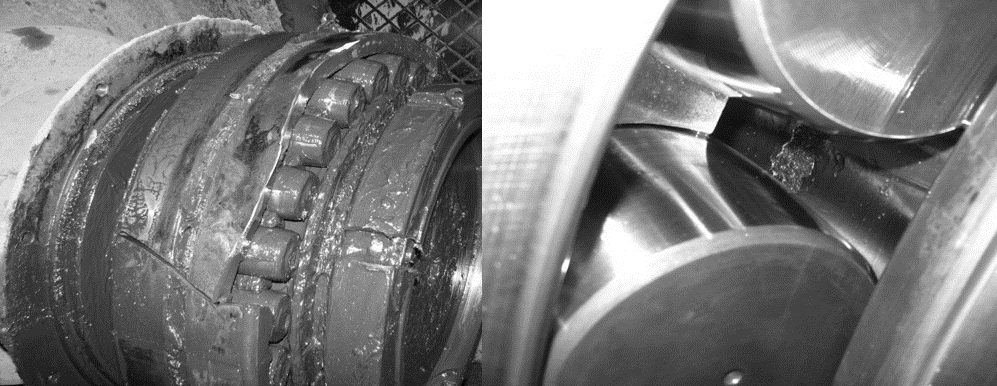
\includegraphics[width = 0.7\textwidth]{wykresy/dmg_race.png}
\caption{Examples of~race damage in~rolling-element bearings, with outer race damage presented on~the~left side, and inner race on~the~right side.}
\label{fig: dmg_race}
\end{figure}

\begin{figure}[ht!]
\centering
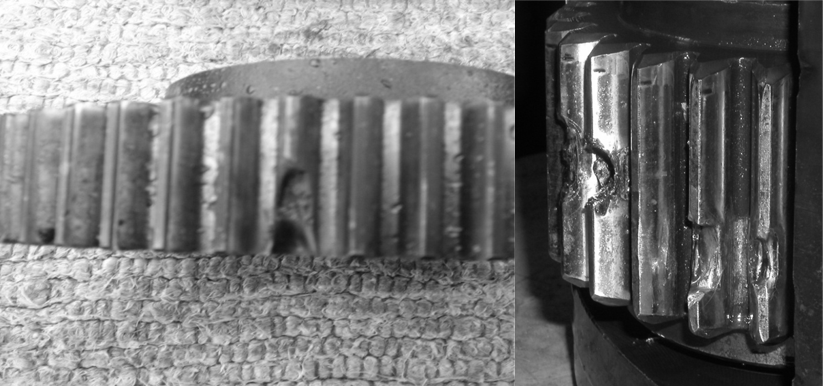
\includegraphics[width = 0.7\textwidth]{wykresy/dmg_tooth.png}
\caption{Examples of~tooth damage in~gearwheels.}
\label{fig: dmg_tooth}
\end{figure}

\begin{figure}[ht!]
\centering
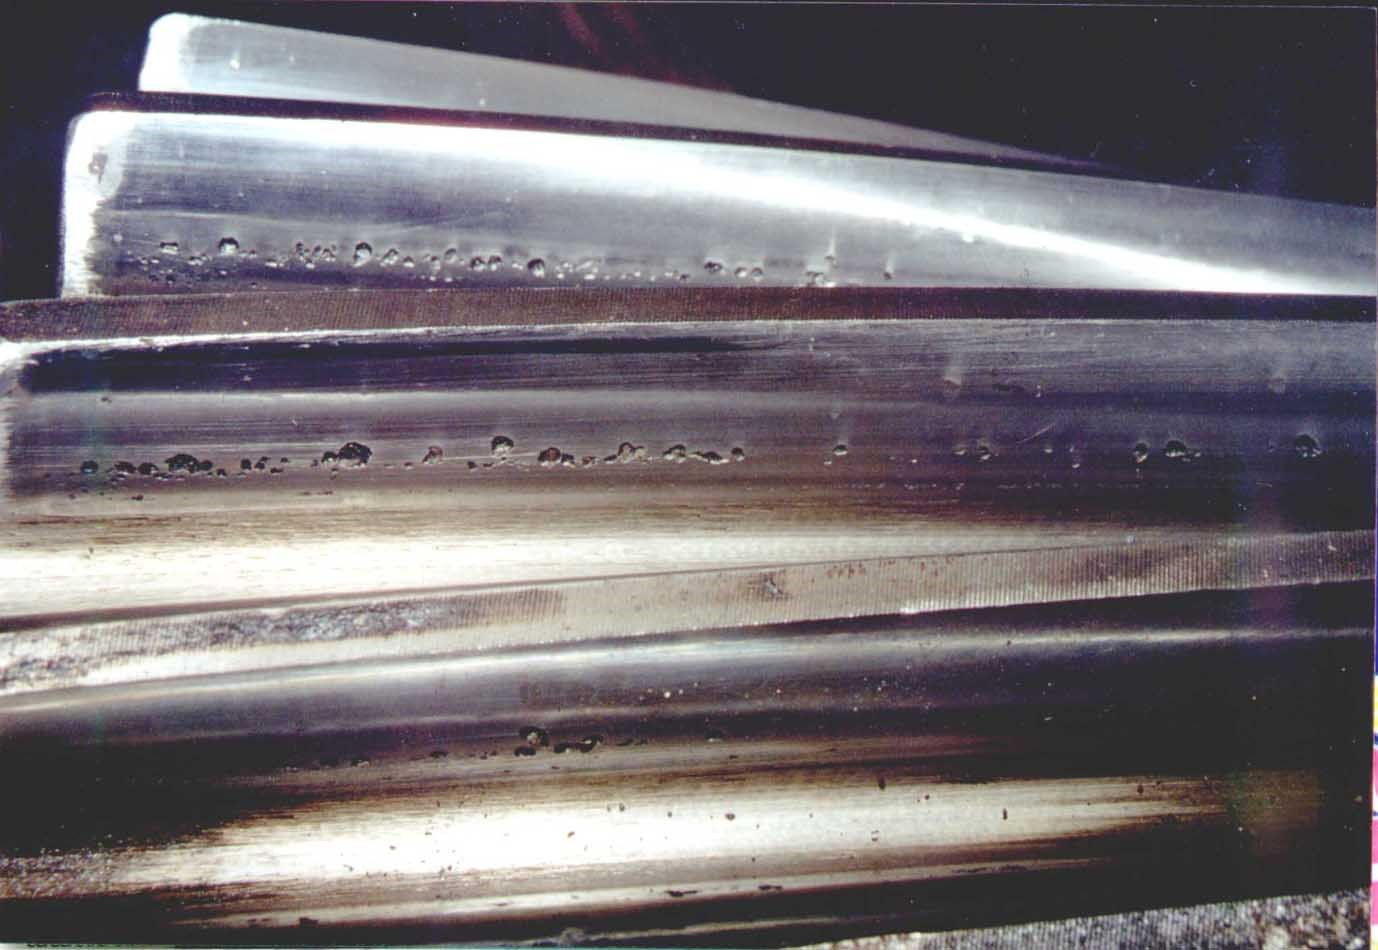
\includegraphics[width = 0.6\textwidth]{wykresy/pitting.jpg}
\caption{Example of~teeth pitting.}
\label{fig: dmg_pit}
\end{figure}

% szumy
Signals generated by~laboratory test rigs will typically include only Gaussian noise. Hence, those signals are expected to~be very easy to~be analyzed, and most of~the~classic techniques are completely enough for conducting investigations in~such conditions. The other type of~signals are the~ones measured in~the~real-life scenarios, and the~feature that distinguishes them from the~laboratory-produced ones is~an~impulsive noise, that can be~expected. It can originate from the~nearby events of~different causes (objects hitting the~machine casing, random disturbances etc.) severely affecting the~overall measurement. 

Vibration signal analysis is~actually one of~the~easiest non-invasive methods of~local damage detection in~machines with rotating elements. Since it~is~sampled relatively frequently in~comparison to~other types of~data measured on~the~industrial machinery, it~can carry a~lot of~important information, especially considering that the~inherent property of~the~operation of~machines with rotating elements is~the~natural occurrence of~cyclic or even periodic behavior. It allows to~use Fourier-based frequency-related analytical mindset as~a~general approach to~processing such type of~data. This feature is~especially convenient due to~the~fact that SOI is~typically connected to~modulations, with special emphasis on~impulsive behavior. 

For the~purpose of~this dissertation an~\emph{impulse} can be~understood as~short-time wideband event in~the~signal, that is~generally caused by~some sort of~impact occurring within a~machine, or being a~result of~an~external event. Such event can be~divided into two general classes: artifacts (i.e. rock or any other arbitrary object hitting a~casing of~the~machine) or impulsive noise (i.e. rock pieces falling into the~crusher).

Impulses as~an~evidence of~a~damage are especially convenient because of~the~idea of~resonant frequency bands (RFB). Resonance is~related to~physical construction and structure of~the~machine, however the~most important fact is~that RFB hardly ever occupies the~entire frequency spectrum of~the~analyzed vibration signal. There are always some bands where signal-to-noise ratio (SNR) is~relatively high, which in~practice means that impulses are possible to~be observed, detected and in~general analyzed in~those bands. Hence, such band (not necessarily continuous) is~called \emph{informative frequency band} (IFB), and its identification is~a~very important approach in~the~field of~machine diagnostics.

\clearpage
\section{Temperature signals from mining machines}

Beside the~main interest in~vibration data, temperature signals have been available for the~author to~be analyzed as~well. During doctoral studies author had an~opportunity to~analyze temperature signals in~two particular cases:

\begin{itemize}
	\item Temperature data from gearboxes in~underground mine belt conveyor driving stations;
	\item Temperature of~engine coolant in~LHD machines operating in~underground mines.
\end{itemize}

On a~large scale of~observation, gearboxes operate in~a~way that it~is~possible to~identify specific patterns within the~measured signal. Since the~machine is~stationary, it~is~easy to~put forth the~interpretation that temperature record of~the~machine can on~some level describe the~character of~its operation. 

Because of~the~fact that on~weekends the~excavation is~stopped, horizontal transportation system is~also shut down, which in~turn allows the~gearboxes to~cool down to~the~level of~ambient temperature. This effect can be~interpreted as~the~first cyclic pattern with a~period of~one week. Another pattern characterized by~the~period of~half a~day is~connected to~the~fact that blasting at~the~mining faces is~performed every 12 hours, which translates into every other work shift. For the~time of~blasting, horizontal transportation system is~also being stopped, which again appears in~the~data as~segments of~clearly decreasing temperature. Third pattern with the~period of~6 hours is~connected to~four work shifts per day. After every shift system is~also stopped, but since this pauses are not as~lengthy as~the~previously mentioned ones, temperature decreases connected to~this process are not manifesting themselves that strongly. One cannot however neglect this effect in~the~assumptions, especially due to~the~fact that it~is~still visible and contributes to~the~overall signal structure.

Considering those three cycles it~is~impossible to~treat this signal as~stationary, especially with respect to~the~mean value. Consequently, methods prepared for the~analysis of~such signal have to~allow nonstationary input, or even assume its cyclostationarity.

Structure of~the~engine coolant temperature measured on~LHD machines is~more complicated and cannot be~analyzed in~terms of~long-term cycles on~the~scale of~days or weeks. In this case shape of~the~signal depends on~many factors, including but not limited to:

\begin{itemize}
	\item Route that the~machine takes at~a~particular shift;
	\item Changes of~the~ambient temperature along the~route when driving from one area to~another;
	\item Operators driving style;
	\item Operation style during a~particular shift (LHD operating with the~support of~hauling truck or not);
	\item Unexpected stoppages during driving;
	\item External human element in~general (presence of~other people or vehicles on~the~route, waiting in~queue for the~dumping screen, other unexpected delays);
	\item Difficulties during loading or unloading;
\end{itemize}

Considering all of~the~uncertainties regarding signal determinism, the~difficulties connected to~the~analysis of~such signal are understandable.

In terms of~temperature data analysis, it~is~easy to~identify overheating as~a~main problem with the~machine. Unfortunately, it~is~defined in~terms of~temperature signal exceeding the~predefined threshold or not. However, such method of~evaluation is~fundamentally incorrect, because temperature data is~fluctuating constantly. Described problem requires methods that do not simply assess the~temperature excess, but take into consideration, e.g. data distributions, signal shapes and structures etc.

\section{The aim of the dissertation}

Based on the analysis of the state of the current knowledge and the personal experience, author presents the following claims:

\begin{itemize}
    \item Utilization of multiple channels of the measurement is a valuable advantage that allows to obtain more complete information than in case of a single-channel measurement. Information in a single channel is very often incomplete or uncertain. Multichannel data enables the information to complement itself between the channels, which improves not only the ease of analysis but also the reliability of the obtained results.
    \item The analysis of multidimensional data representations can provide better insight into the component features or events occurring in the signal. It is especially important considering the fact that very often the sought information is strongly suppressed by high-energy noise present in the real-life measurements. Beside the noise itself, even the components describing the ordinary operation of the machine can make the fault information discovery very difficult.
    \item The most advantageous case happens when a multidimensional diagnostic data is available, and its character allows to utilize multidimensional techniques for detailed investigation of the fault-related signal components.
\end{itemize}

The following work is aimed at addressing the issues imposed by real-life industrial data analysis taking advantage of multiple channels of measurement of diagnostic data, using multidimensional analytical techniques when it is possible, and in the most advantageous cases combine those approaches to maximize the reliability and quality of obtained diagnostic information.
\cleardoublepage


\chapter{Objects and experiments}

During the~course of~doctoral studies author has conducted his research based on~data acquired on~various types of~mining machines at~various stages of~the~production process. Considered objects included static machines (e.g. gearboxes and electric engines of~belt conveyors, bearings of~crusher shaft, belt conveyor drive pulley and oil rig gas compressors) as~well as~mobile ones (Load-Haul-Dump machines, haulage trucks, roadheader). Every object has its specific features and is~influenced differently by~the~operational and environmental conditions. Moreover, objects suffer differently from degradation processes specific to~their type.

\section{Objects of~interest for vibration data analysis}

Measurements on~regarded objects were performed using different data acquisition systems. This way, it~was possible for the~author to~acquire the~experience regarding the~analysis of~vibration signals that have different parameters. The most important acquisition systems for the~purpose of~author's work were:

\begin{itemize}
  \item \textbf{DiagManager}: portable 4-channel data acquisition system designed by~specialists from the~Faculty of~Geoengineering, Mining and Geology for KGHM. Used sampling frequency: 17 kHz 
  \item \textbf{Br{\"u}el \& Kjaer Pulse}: 7-channel portable data acquisition system. Used sampling frequency: 8192 Hz, 16384 Hz
  \item \textbf{NI-DAQ}: portable 2-channel data acquisition system based on~NI-DAQ data acquisition card and SignalExpress environment from National Instruments. Used sampling frequency: 25 kHz.
  \item \textbf{Pr{\"u}ftechnik}: bulit-in data acquisition system. Used sampling frequency: 19200 Hz.
  \item \textbf{EC Group}: bulit-in live monitoring system. Used sampling frequency: 24 kHz.
\end{itemize}

Failures encountered in~investigated machines contained meshing degradation on~the~gear wheel of~the~first shaft and tooth breakage on~the~gear wheel of~the~second shaft.

% Vibrations belong to~the~class of~fast-changing processes that require high sampling frequency for proper data acquisition. Taking advantage of~relatively fast sampling of~measured signals, one can perform certain types of~analysis, that capitalize on~the~small impact of~missing information. For signal processing tasks related to~damage detection and diagnostics in~general, methods of~favor include i.e. spectral-related analysis. Frequency-related methods also happen to~be very suitable for machine diagnostics, hence frequencies (or periods) that are present in~the~acquired vibration signals are directly related to:

% \begin{itemize}
%   \item Expected cycles related to~normal operation of~the~machine;
%   \item Periodic or otherwise cyclic components related to~local damage that occurred on~one of~the~elements of~the~machine.
% \end{itemize}

% Such an~assumption is~very promising, especially considering that machines with rotating elements are subjects of~the~majority of~the~analytical methods described in~this thesis.

\subsection{Gearbox in~belt conveyor drive}

In case of~the~belt conveyor drive unit the~purpose of~the~diagnostic experiment was to~acquire vibration signal from the~heavy-duty gearbox operating in~the~driving station (see Fig. \ref{fig:obj_gear}). 

% \begin{figure}[ht!]
% \centering
% 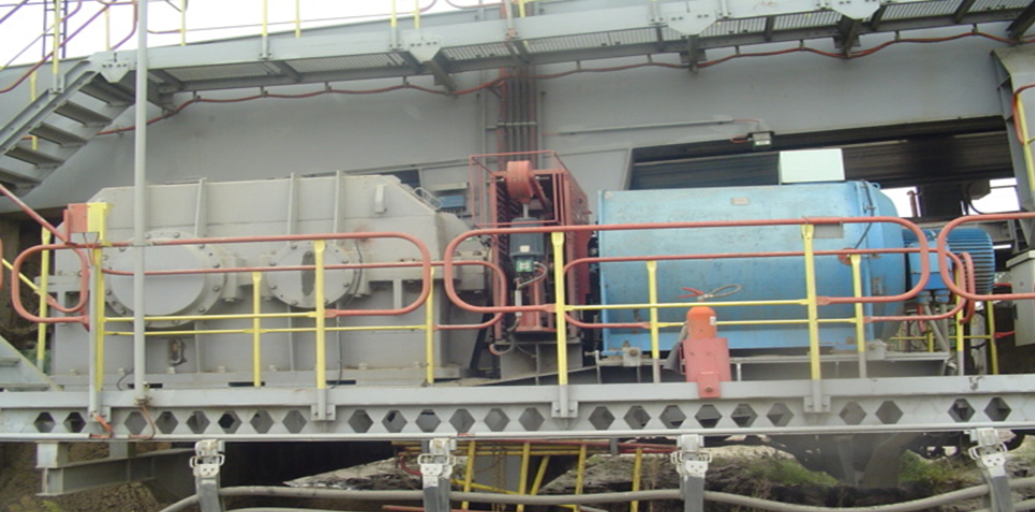
\includegraphics[width=0.7\textwidth]{wykresy/obj_gear.png}
% \caption{Two-stage gearbox operating in~the~driving station}
% \label{fig:obj_gear}
% \end{figure}

\begin{figure}[!ht]
 \centering
 \begin{subfigure}
   \centering
   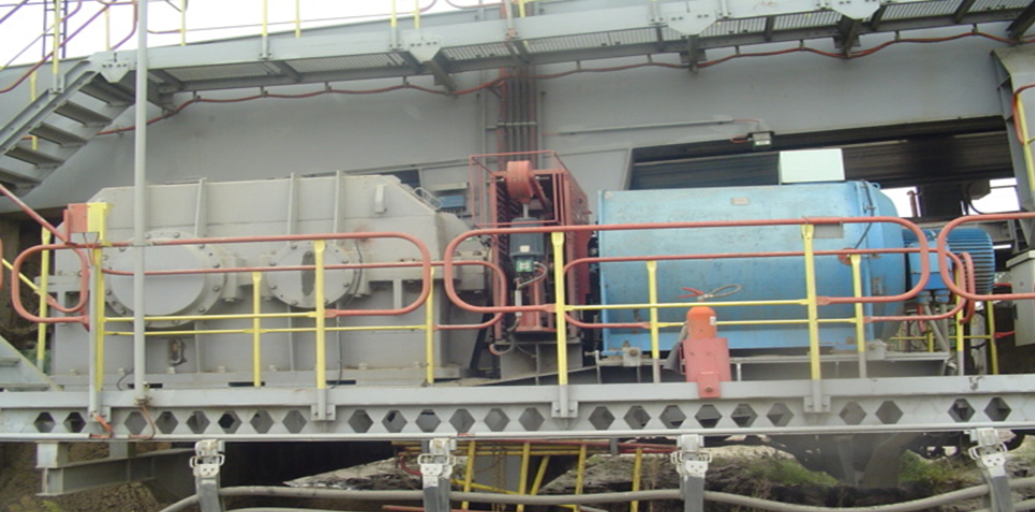
\includegraphics[width=0.48\textwidth]{wykresy/obj_gear.png}
 \end{subfigure}
 \begin{subfigure}
   \centering
		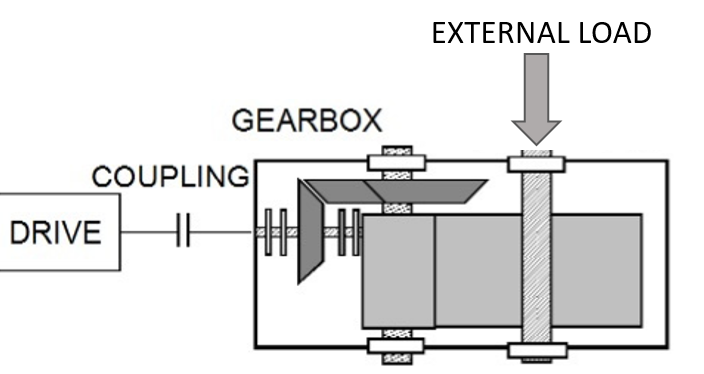
\includegraphics[width=0.48\textwidth]{wykresy/gb_sch2.png}
 \end{subfigure}
 \caption{Two-stage gearbox (left panel) and simplified schematic of~driving station (right panel)}
 \label{fig:obj_gear}
\end{figure}



Depending on~the~design (required power for driving of~belt conveyor), belt conveyor driving station might consist of~one up to~four drive units with 630 or 1000 [kW] power each. In this case a~two-stage gearbox has been diagnosed, with conical stage at~the~input and cylindrical one on~the~output. Characteristic frequencies present in~the~operation of~the~machine are shown in~Table \ref{tab: obj_gear}.

\begin{table}
	\begin{center}
		\begin{tabular}{|c|l|l|l|}
			
			\hline
			No & Notation & Description & Value/unit \\ \hline
			1 & $f_{01}=\frac{n_1}{60}$ & Rotational frequency of~the~first shaft & 16.58 Hz \\ \hline
			2 & $f_{02}=\frac{n_2}{60}=\frac{n_1}{60 \cdot u_1}$ & Rotational frequency of~the~second shaft & 4.1 Hz \\ \hline
			3 & $f_{03}=\frac{n_3}{60}=\frac{n_1}{60 \cdot u_1 \cdot u_2}$ & Rotational frequency of~the~third shaft & 1.31 Hz \\ \hline
			4 & $f_{z_{12}}=\frac{n_1 \cdot z_1}{60}$ & Gear mesh frequency of~the~first stage & 381.42 Hz \\ \hline
			5 & $f_{z_{34}}=\frac{n_2 \cdot z_2}{60}$ & Gear mesh frequency of~the~second stage & 147.6 Hz \\ \hline
			6 & $U_p=\frac{z_2 \cdot z_4}{z_1 \cdot z_3}$ & Ratio & 12.69 \\ \hline
			
		\end{tabular}
	\end{center} 
	\caption{Gearbox characterietic frequencies}
	\label{tab: obj_gear}
\end{table}

\subsubsection{Experiments}
Several measurements have been conducted using Br{\"u}el \& Kjaer Pulse portable measurement system. For each measurement the~signal was acquired with the~sampling frequencies set to~$f_s = 8192$ and 16384 Hz and duration T = 2.5 s. Failures encountered in~investigated machines contained meshing degradation on~the~gear wheel of~the~first shaft and tooth breakage on~the~gear wheel of~the~second shaft.

\subsection{Rolling bearing in~a~belt conveyor drive pulley}

The bearing under investigation is~23264 CCK/W33 type two row spherical roller bearing with outer diameter equal to~830 mm and inner diameter 500 mm. Each row contains 24 rolling elements, 48 in~total. Based on~the~bearing geometry and the~shaft’s rotational speed, it~was possible to~calculate the~characteristic defect frequencies of~the~rolling bearing, see Table \ref{loz_table}.

\begin{figure}[ht!]
\centering
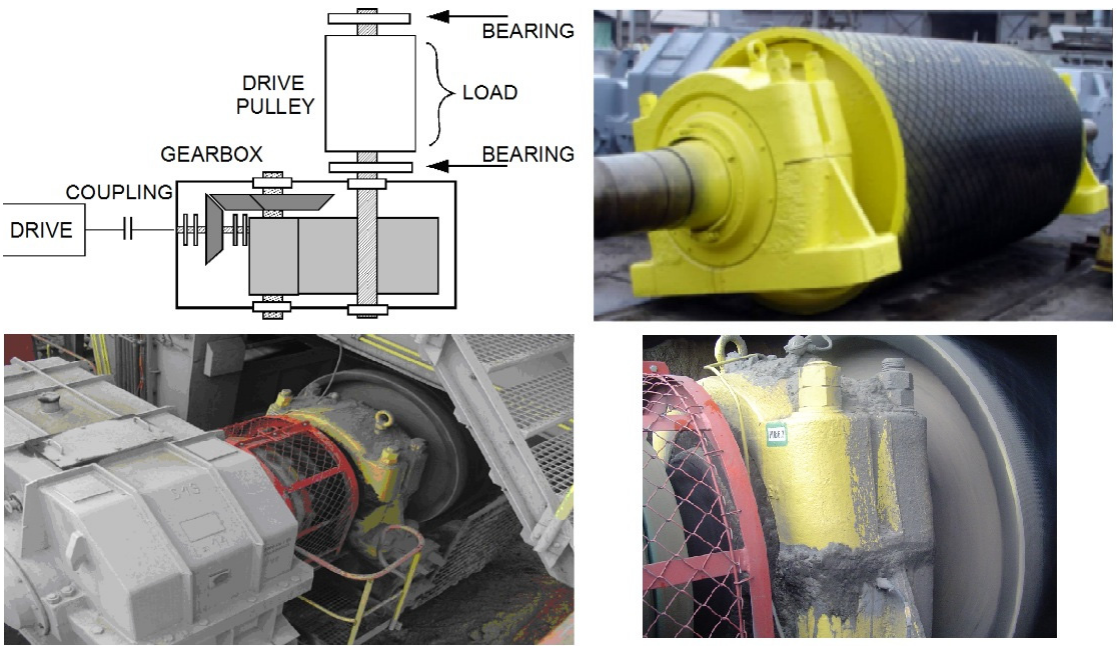
\includegraphics[width=0.9\textwidth]{wykresy/gb.PNG}
\caption{Rolling bearing location in~the~driving station}
\label{fig:gb}
\end{figure}

Fig. \ref{fig:gb} presents the~schematic of~the~drive unit for a~belt conveyor with the~indication where the~bearings are operating. The drive unit consists of~an~electric motor, a~coupling and two stage gearbox, that are connected with a~pulley.

\begin{table}
\begin{center}
	\begin{tabular}{|c|l|l|l|}
		\hline
		No & Notation & Description & Value/unit \\ \hline
		1 & $f_{FTF}$ & Fundamental train frequency & 0.51 Hz \\ \hline
		2 & $f_{BSF}$ & Ball spin frequency & 4.45 Hz \\ \hline
		3 & $f_{BFF}$ & Ball fault frequency & 8.9 Hz \\ \hline
		4 & $f_{BPFO}$ & Ball passing frequency outer race & 12.69 Hz \\ \hline
		5 & $f_{BPFI}$ & Ball passing frequency inner race & 16.06 Hz \\ \hline
		
		%\caption{Bearing frequencies: 23264 CCK/W33}
	\end{tabular}
\end{center} 
\caption{Bearing frequencies: 23264 CCK/W33}
\label{loz_table}
\end{table}


% The pulley consists of~a~shaft, two bearings and the~coating covered by~rubber (to increase friction between the~pulley coating and the~belt). Often between the~gearbox and the~pulley a~rigid coupling is~used.
\subsubsection{Experiment}

Several measurements have been conducted using Pr{\"u}ftechnik online measurement system. For each measurement the~signal was acquired with the~ sampling frequency $f_s = 19.2$ kHz and duration T = 2.5 s. Fault of~the~investigated bearing has been identified as~a~local damage on~the~outer race.

\subsection{Reciprocating gas compressor}

The studied machine is~a~1000 kW reciprocating gas compressor of~a~type Dresser-Rand C-VIP, operating between 600-1000 rpm, with a~four-stage compression \cite{barszcz2013bearings}. The machine operates on~the~offshore oil rig. The key issue is~that vibration signals generated by~the~compressor contain a~number of~external disturbances, the~most influential being the~piston-related and valve-related ones. 

\begin{table}[ht!]
  \centering
  \caption{Machine-related frequencies for investigated compressor}
  \begin{tabular}{|l|l|}
  \hline
     \textbf{Parameter} & \textbf{Frequency [Hz]} \\ \hline
     Sampling frequency & 24000 \\ \hline
     Shaft speed & 12.35 \\ \hline
     BPFI & 127.9 \\ 
  \hline
  \end{tabular}
  \label{tab:tab1}
\end{table}

\begin{figure}[ht!]
\centering
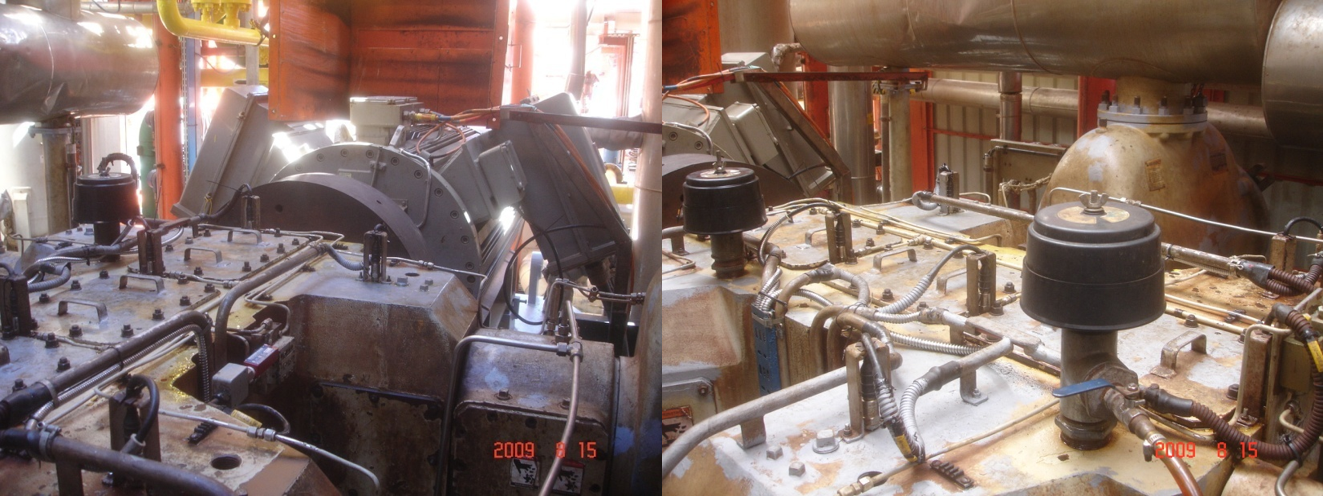
\includegraphics[width=0.8\textwidth]{wykresy/obj_komp.png}
\caption{Reciprocating gas compressor operating on~the~oil rig}
\label{fig:obj_komp}
\end{figure}

\subsubsection{Experiment}

Vibration measurement has been performed using on-board live monitoring system with sampling frequency $f_s=24$ kHz. It has been discovered that the~analyzed signal has been recorded when the~inner ring has been severely defected in~one of~the~main shaft bearings. Details including the~SOI parameters are presented in~Table~\ref{tab:tab1}.

\subsection{Copper ore crusher in~mineral processing plant}

The machine under investigation is~a~copper ore hammer crusher operating in~mineral processing plant (see Figure \ref{fig:obj_crusher}). Analysis of~vibration signal measured on~such machine is~very challenging from the~signal processing point of~view. The difficulty lies in~the~way that the~machine operates. Rock pieces falling into the~machine from the~top hit the~walls in~a~random way, which generates very strong impulses. Similar impulses are caused by~the~hammers crushing the~pieces. In terms of~stochastic modeling it~is~a~non-Gaussian noise. It is~described as~a~noise because it~occurs randomly, and it~is~non-Gaussian, because it~has relatively high probability of~high values not associated with Gaussian distribution, that manifest as~mentioned impulses. Considering the~presence of~such noise it~is~very difficult to~be able to~detect modulations related to~damage on~one of~the~elements, because corresponding cyclic component is~expected to~also be~impulsive, but much less energetic.

\begin{figure}[ht!]
\centering
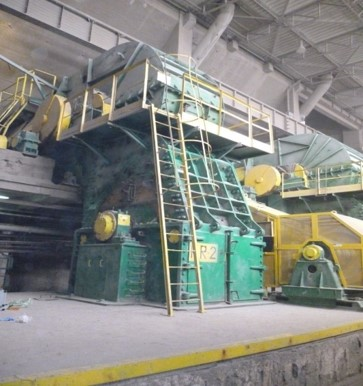
\includegraphics[width=0.5\textwidth]{wykresy/obj_crusher.jpg}
\caption{Copper ore crusher}
\label{fig:obj_crusher}
\end{figure}

\begin{table}
	\begin{center}
\begin{tabular}{|c|l|l|l|}
	\hline
   No & Notation & Description & Value/unit \\ \hline
	1 & $n_i$ & Rotational speed of~the~inner ring & 180 RPM \\ \hline
	2 & $F_i$ & Rotational frequency of~the~inner ring & 3 Hz \\ \hline
	3 & $F_c$ & Rotational freq. of~the~rolling element and cage assembly & 1.3 Hz \\ \hline
	4 & $F_r$ & Rotational freq. of~a~rolling element about its own axis & 10.6 Hz \\ \hline
	5 & $F_{ip}$ & Over-rolling frequency of~one point on~the~inner ring & 30.7 Hz \\ \hline
	6 & $F_{ep}$ & Over-rolling frequency of~one point on~the~outer ring & 23.3 Hz \\ \hline
	7 & $F_{rp}$ & Over-rolling frequency of~one point on~a~rolling element & 21.1 Hz \\ \hline
\end{tabular}
\end{center} 
\caption{Bearing frequencies from copper ore crusher}
\label{krusz_table}
\end{table}

\subsubsection{Experiment}
The considered element was 23264 SKF bearing. Vibration data has been measured in~two orthogonal directions with Endevco accelerometers, and signal acquisition was based on~NI-DAQ card and LabView Signal Express environment. Sampling frequency of~vibrations signals is~25 kHz. The particular vibration signal considered in~this dissertation is~a~10-second section of~the~60-second measurement session. Characteristic frequencies of~the~bearing are presented in~Table \ref{krusz_table}. Fault of~the~investigated bearing has been identified as~a~local damage on~the~inner race.


\section{Objects of~interest for analysis of~other types of~data}
 
Vibration data analysis is~a~very important component of~this dissertation, however it~is~not the~only type of~data under investigation. Hence, in~this section author describes the~machines that have provided other types of~data. This group contains the~gearbox of~conveyor belt drive and self-propelled load-haul-dump wheeled machine (LHD). 

\subsection{Load-Haul-Dump machines in~underground mine}

Load-haul-dump machines (LHD, a.k.a. \emph{loaders}, see Figure \ref{fig:obj_lhd}) are key assets used in~Polish copper ore mines. They are designed to~load blasted ore from mining face onto haulage trucks, or transport ore to~the~screen by~themselves. Reliability and effectiveness of~those machines have a~huge impact on~the~overall performance of~the~production. LHD machines along with their maintenance are also one of~the~most expensive aspects of~underground mining. Strongly time-varying and harsh operating conditions determine high workload, that in~connection with high effectiveness and availability demands are a~big challenge for maintaining their technical condition on~the~highest level possible.

\begin{figure}[ht!]
\centering
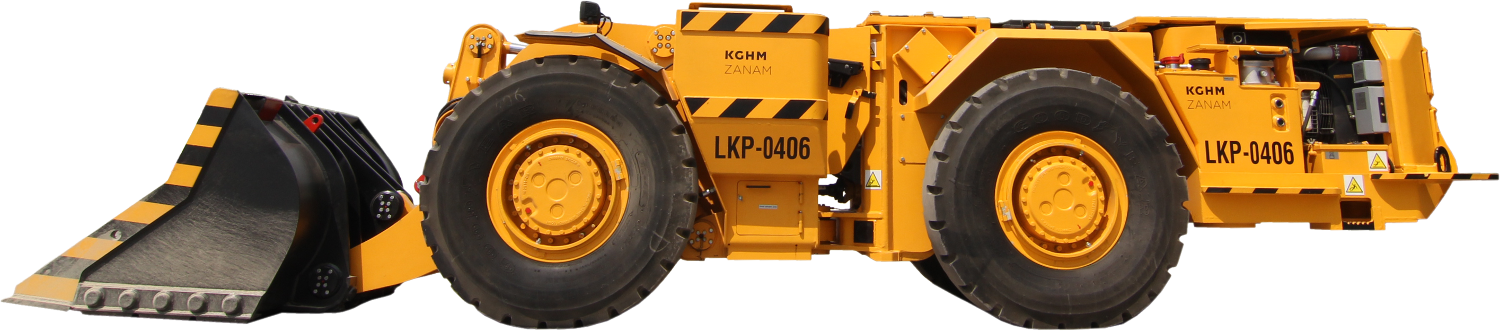
\includegraphics[width=\textwidth]{wykresy/obj_lhd.png}
\caption{Self-propelled Load-Haul-Dump machine}
\label{fig:obj_lhd}
\end{figure}

One of~the~most important problems of~those machines is~overheating, hence temperature data recorded from LHD-s is~very important in~the~condition monitoring process. However during the~operations of~loading temperature itself strongly varies, which is~closely related to~technical condition, operating load and harsh mining conditions, but also the~fact that the~machine can perform various tasks and take different route during every work shift. In this case the~analysis of~temperature data is~very difficult especially in~the~long term, because there is~virtually no control over the~details of~the~process from the~point of~view of~data acquisition being interpreted as~an~experiment. 

\subsubsection{Experiment}
Diagnostic data is~registered using on-board acquisition system installed by~the~manufacturer. Beside the~engine coolant temperature analyzed in~this dissertation there is~a~lot of~other parameters being registered on~the~LHDs, including but not limited to:
\begin{itemize}
  \item pressures of~engine oil, gearbox oil, oil in~hydraulic actuation system etc.,
  \item temperatures of~engine oil, gearbox oil, oil in~hydraulic actuation system etc.,
  \item rotations per minute of~the~engine shaft,
  \item speed of~the~vehicle.
\end{itemize}

Individual parameters can be~sampled with different frequencies, but for the~purpose of~saving the~storage space all of~sampling frequencies are set by~default to~1 Hz. In case of~certain parameters describing fast-changing processes it~could be~a~disadvantage, however, since temperature is~a~case of~slowly-changing process with inherent inertia, analytical methodology does not suffer from the~relatively slow sampling. Moreover, such configuration allows to~store records from the~entire lifetime of~the~machine in~the~databases of~the~owning company.

In case of~the~analyses presented further in~this dissertation author uses the~variable describing the~temperature of~the~engine coolant, further referred to~as \emph{temperature data}. Available record spanned over the~period of~2,5 months. During this period the~machine was performing tasks typical for its purpose, such as~picking up blasted material from the~mining face and transporting it~to~the~dumping screen in~case of~operating on~its own, or dumping the~material to~the~bucket of~haulage truck in~case of~work in~conjunction.

\subsection{Gearbox in~underground belt conveyor drive}

Vibration data is~generally considered to~be a~better source of~diagnostic information than temperature for many reasons:

\begin{itemize}
  \item the~information about occurring events is~instantaneous,
  \item signal has broader bandwidth, hence it~is~richer in~useful components,
  \item all the~information is~aggregated, and in~practice impossible to~be decomposed in~a~way that vibration data can be, because of~the~insufficient bandwidth.
  \item it~is~possible to~observe processes much weaker in~energy that are not manifesting themselves in~the~temperature data etc.
\end{itemize}

Unfortunately, it~is~not always possible to~obtain it. In most cases machines are not equipped with built-in vibration acquisition system, and to~perform the~measurement it~is~necessary to~send a~person equipped with a~portable measurement system. On the~other hand, much more machines have built-in capability to~record temperature data because of~the~installed monitoring systems.

In many cases failures of~gearboxes are manifested by~overall machine overheating. However gearboxes operating in~belt conveyor drives, as~well as~belt conveyors as~a~whole, can be~considered as~time-varying system and direct decision making using direct readout of~parameters can be~very difficult. To address this issue, long-term analysis of~records such as~temperature enables to~learn how to~recognize alarming moment. Thus the~maintenance tasks can be~better scheduled to~minimize the~stoppages and losses in~production. 

\subsubsection{Experiment}
Temperature is~measured on~gearbox casing using SCADA system used continuously by~the~mining company. Data sampling is~not fixed, the~next sample is~recorded when the~temperature exceeds predefined resolution threshold with respect to~the~previous sample. Such approach allows to~use less storage space for the~registered data. However, many analytical techniques require even data sampling, so resampling procedures are very often a~necessary preprocessing step for such data.

In case of~temperature record analyzed in~this dissertation, data spans over the~period of~72 days, when the~machine was operating in~its typical manner described described more in~section \ref{temp_em}. 
\cleardoublepage
\chapter{State of~the~art}

Local damage detection at~the~early stage of~development is~one of~the~most important tasks in~modern condition monitoring. Management of~the~machines is~heavily influenced by~this aspect, which utilizes broad spectrum of~methods, often interdisciplinary ones. Since author focuses on~fault detection based on~vibration and temperature data, this chapter is~divided into two parts.

\section{Vibration-based damage detection}
Multiple works focused on~the~local damage detection in~the~bearings and gearboxes can be~found in~the~literature. It was proven by~Cempel, Jonak and many other authors that multidimensional analysis for condition monitoring, especially under nonstationary operations is~very interesting and fruitful approach \cite{cempel2007multidimensional,zimroz2013two,bartkowiak2014dimensionality,zimroz2014diagnostics,jedlinski2015early,jedlinski2017disassembly}. 

% bartelmus
In the~field of~industrial machine diagnostics, one can find multiple different types of~devices. One of~the~most difficult types to~analyze are those working in~highly nonstationary conditions. Bearings of~such machines are exposed to~high amount of~stress and often tend to~wear very quickly. Difficulty in~analysis of~such signals comes from the~variation of~vibration-based diagnostic features caused mostly by~load/speed variation and low signal-to-noise levels. Zimroz, Bartelmus, Barszcz and Urbanek in~\cite{zim_barszcz_mssp} proposed method based on~the~statistical patter recognition for bad and good condition of~the~bearings. Authors have extended this method by~load susceptibility characteristics as~a~feature. Interesting work has been also presented by~Burdzik where authors discuss multidimensional techniques for the~analysis of~nonstationary vibration signals from the~automotive and transportation industry \cite{burdzik2019multidimensional,burdzik2018application,burdzik2013research}.

Paper that is~still one of~the~most important ideas in~the~field is~\cite{bartelmus}. In this article, authors introduced new diagnostic feature which could be~used in~time-varying operating conditions. This method exploits the~fact that a~planetary gearbox in~bad condition is~more susceptible to~load than a~gearbox in~good condition. One needs to~capture signals for different external load values and calculate a~simple spectrum based feature versus operating conditions indicator (current or instantaneous rotation speed). In a~certain range of~operating conditions the~diagnostic relation (i.e. the~dependence between the~spectral features and the~operating conditions indicator) is~linear. However, since a~gearbox in~bad condition is~more susceptible to~load than the~gearbox in~good condition the~relation will be~different for the~two cases. Using a~simple regression equation one can calculate the~slope of~the~straight line, which expresses the~new diagnostic feature.

One of~the~most prolific reviews in~the~field was put forth by~Samuel and Pines \cite{samuel_pines}. It recapitulates over two decades of~development of~the~diagnostic algorithms for the~gearboxes. It describes widely used statistical measures for the~signal energy. Moreover, authors compare application of~various time-frequency representations such as~spectrogram or Wigner-Ville distribution for the~problem of~local damage detection \cite{forrester, forrester2, samuel2, nasa1}. 

% podstawy bearings
McFadden and Smith \cite{mcfadden_bearings} presented one of~the~most significant research pieces regarding the~local damage detection of~the~bearings. The investigated the~high-frequency resonance approach, as~suitable for the~vibration-based monitoring of~gearboxes because of~the~possibility to~separate the~signature of~a~defective bearing from the~rest of~the~signal. Another interesting techniques regarding fault detection in~bearings were published in~\cite{AYE20151779,COCCONCELLI2012667}.

% Time averaging 
Time-synchronous averaging is~another successful method that is~commonly used in~the~field. Vibration signal is~averaged within periodic sections, which unfortunately requires prior knowledge of~the~correct period, that can be~a~disadvantageous property regarding the~robustness of~the~procedure \cite{braun_tsa,Wang201774}.  In the literature one can also find application of the transient signal analysis and unsupervised classification \cite{TIMUSK20081724} for local damage detection in industrial machinery. 

%STFT
Very often time-frequency representations serve as~a~basis for multidimensional diagnostic procedures based vibration data analysis, with Short-Time Fourier Transform being arguably the~most popular one \cite{oppenheim1999discrete}. a~modification of~the~STFT representations was proposed by~Obuchowski in~\cite{obuch3}. The problem is~that in~most (if not all) of~the~industrial cases signal-to-noise ratio is~very low. Damage-related modulations are buried deep in~high energy of~the~background noise. In order to~deal with this issue, authors have proposed the~local maxima approach. It is~based on~looking for the~local maxima in~the~spectrogram. Proper derivation of~the~weight vector for the~spectrogram can significantly improve visibility of~the~impulsive components. 

% falki
Wavelet analysis is~another topic strongly expanded in~the~recent years \cite{WANG1996927, staszewski, samuel3}. An~interesting approach was presented in~\cite{linzuo}, where an~adaptive filter based on~the~Morlet wavelet has been developed. Adaptiveness of~the~wavelet is~achieved by~allowing the~parameters to~not be~fixed. In \cite{rozsz_jve_16} Peng and Chu review the~wavelet-related techniques used in~the~field of~condition monitoring. In \cite{WANG1996927} Wang and McFadden proposed the~application of~this method for fault detection in~helicopter gearboxes. Miao and Makis \cite{MIAO2007840} have investigated an~interesting approach that utilizes both probabilistic and wavelet techniques. They have classified the~machinery state, for such knowledge allows one to~schedule appropriate maintenance in~practice based on~the~hidden Markov models and validation using wavelet modulus maxima distribution. Another research concerning application of~wavelets and time-frequency decomposition were presented in~\cite{ALBADOUR20112083, RUBINI2001287}. In \cite{combet2012novel} Gelman and Combet propose a~technique called instantaneous wavelet bicoherence in~application to~vibration measurements for local damage detection in~gears. It allowed to~detect gear pitting in~both experimental and real-life scenarios. Presented technique demonstrated superior capablities over the~conventional detection methods based on~the~wavelet transform. In \cite{peter2001wavelet} Tse presents the~application of~wavelet analysis to~the~problem of~rolling element bearing diagnostics, and in~\cite{PENG2005974} compares wavelet transform to~Hilbert-Huang transform in~application to~the~same problem.

% Cyclo
Other class of~tools for information discovery are so-called cyclostationary maps: cyclic spectral coherence (CSC), cyclic spectral density (CSD) and cyclic modulation spectrum (CMS) \cite{antoni3}. Cyclic modulation spectrum is~bi-frequency representation defined as~a~combination of~Fourier transforms of~instantaneous power spectra of~the~signal calculated using discrete Fourier transforms of~the~absolute value of~the~STFT. Another bi-frequency map is~a~cyclic spectral density, defined as~a~correlation density of~two spectral components spaced apart by~frequency $\alpha$ in~the~vicinity of~the~central (carrier) frequency \textit{f}. If the~spacing is~equal to~0, CSD reduces to~the~ordinary power spectrum. Finally, cyclic spectral coherence is~a~normalized CSD. All of~described representations play an~important role in~cyclostationarity analysis in~the~signals. However, their main disadvantage is~the~fact that they use the~second moment which can be~undefined for the~impulsive behavior of~the~data. 

% SCD
One of~the~most recent approaches to~damage detection was put forth by~Urbanek \cite{urbanek2014integrated}, \cite{URBANEK2012399} where authors studied generalization of~the~spectral correlation density, known as~modulation intensity distribution. Authors have investigated its functionality as~a~descriptor for detection of~the~presence of~rolling element bearing faults in~noisy environments. 

% SK
Significant amount of~research conducted in~recent years was aimed at~the~fault detection in~the~presence of~Gaussian noise. Antoni and Randall have put forth very interesting approach based on~very simple statistic \cite{antoni_randall}. This presents a~detection method using spectral extension of~the~sample kurtosis. In such a~way it~can represent a~filter magnitude characteristics or a~tool for informative frequency band selection within which further analysis should be~conducted. However, it~assumes the~additive Gaussian noise in~the~signal, so its application is~limited to~theoretical considerations. In addition kurtosis is~very sensitive to~rare or even singular impulses known as~artifacts, which additionally jeopardizes the~correctness of~the~results. 

Spectral kurtosis could also serve as~a~tool to~construct optimal Wiener filter as~shown by~Gelman and Combet \cite{combet2009optimal}. Authors applied it~to~gear residual signal after removing meshing component, which allowed to~detect surface pitting on~early stage of~development.

% Kurtogram
Modification of~the~spectral kurtosis method is~a~kurtogram \cite{antoni2007fast}. It is~based on~the~biforcation of~frequency domain into gradually smaller subbands. Input data is~then processed with a~bandpass filter corresponding to~a~particular subband and kurtosis of~the~result is~calculated. Composition of~those kurtosis values into the~array of~kurtogram allows user to~define the~most impulsive subband. However, the~disadvantages of~the~kurtosis persist. 

%Protrugram
Kurtogram was also a~basis for the~design of~the~techniques that will not suffer from singular impulses. Study put forth by~Barszcz and Jabłoński in~\cite{barszcz_mssp} with singular impulse influecing the~kurtogram-related analysis proved it~to~be very ineffective in~the~presence of~random disturbances. Hence, the~enhanced version of~the~kurtogram was developed by~the~name of~protrugram. It relies on~the~kurtosis of~the~envelope spectra instead the~kurtosis of~the~filtered time series.

%zaku
Antoni and Borghesani in \cite{BORGHESANI2017378} investigated the influence of the $\alpha$-stable noise on the traditional statistical estimators, and proposed log-envelope analysis as a countermeasure to nonexistent second moments. An interesting approach of vibration-based damage detection inspired by those studies was presented by Żak. In \cite{11419466920160301} he proposed to use the parameters of $\alpha$-stable distribution as a basis to construct a custom selector either to serve as a filter for the input data, or as an indicator of the informative frequency band. He also proposed to use a multidimensional data representation based on time-frequency representations, called Fractional Lower-Order Covariance (FLOC), for the purpose of machine diagnostics \cite{Zak2014}. It exhibits advantageous properties in comparison to classic time-frequency representations, because of the focus on enhancing periodic features.

Besides damage detection specifically, wear monitoring and detection in~rotating machinery is~another very important aspect of~diagnostics. Heyns et.al. have presented multiple examples of~analytical techniques based not only on~vibration data analysis, but also fusing it~with other features, e.g. strain measurement, angular speed etc. \cite{stander2002using,scheffer2001wear} using techniques such as~order tracking \cite{wang2011combined,wang2012application}, neural networks \cite{herzog2009machine,ngwangwa2014reconstruction}, or Vold-Kalman filtering \cite{wang2009vold,wang2011combined}.

\section{Temperature-based damage detection}

In recent years one can observe increasing interest towards automated temperature-based machine monitoring and diagnostics. Especially in~the~context of~the~philosophy of~the~"Industry 4.0", SCADA systems are becoming more and more common in~industrial facilities, which enables the~implementation of~such solutions \cite{zhang2012research,eliasson2013internet,bongers2008fault,wilkinson2014comparison}.

% coolant temperature modeling
In \cite{junnuri2015engine} Junnuri describes developed an~internal combustion engine coolant temperature model for control and diagnostics development and validation purpose. Authors propose to~use both physical laws and dynamic data to~develop the~dynamic model of~the~cooling system.

In \cite{sawicki2015automatic} Sawicki proposed a~multichannel technique for temperature analysis from belt conveyor gearboxes. Authors utilize Wold's decomposition for model-based anomaly detection. Temperature modeling is~also used by~Guo, Infield and Yang in~\cite{guo2011wind} 
where they propose a~condition-monitoring method based on~the~nonlinear state estimate technique for a~wind turbine generator. Authors construct the~normal behavior model of~the~electrical
generator temperature for the~purpose of~trend analysis for deviation detection. Trend-based anomaly detection was also described in~\cite{astolfi2014fault} with respect to~wind turbines.

In \cite{Nembhard2013} the~method for bearing fault diagnosis based on~the~conjunction of~temperature and vibration data is~presented. Authors indicate that the~usage of~information from both types of~data yields better results than the~method based only on~vibration data analysis \cite{Nembhard2013b}.

An interesting approach to the temperature analysis was presented by Staszewski and Dao in \cite{DAO2018107}. Authors propose to use the approach of SCADA data cointegration applied to wind turbines diagnostic signals. This approach allowed to analyze nonlinear data trends to reliably detect abnormal problems.

Finally, thermographic image analysis is also very potent basis for machine monitoring and diagnostics \cite{Lim2014,5608306}. It is a very powerful approach and as an image-analysis-related method it can be also understood as a multidimensional one, however this approach is not the subject of this dissertation.


\cleardoublepage


\chapter{Novel methodology for damage detection}\label{methodology}

In this chapter of~the~dissertation, author presents the~methodology developed and applied towards simulated and real signals. The elementary techniques of~these methods are known and used in~other areas of~research. However, the~novelty of~this dissertation lies in~designing specific analytical methods utilizing said techniques, that can successfully deal with the~difficulties related to~the~diagnostics of~heavy-duty mining machinery.

\section{Methods for temperature data analysis for technical condition change detection}\label{temps}

Temperature data can be~a~very rich source of~diagnostic information. While being very natural to~understand, its meaning is~also universal across numerous types of~machines. Hence, in~this chapter methods \ref{temp_ica} and \ref{temp_em} regard the~analysis of~temperature data recorded on~the~belt conveyor gearboxes, and on~the~other hand techniques \ref{temp_bulgaria} and \ref{temp_ad} consider temperature data measured on~the~LHDs. 

\subsection{Failure detection using ICA}\label{temp_ica}

In this section, author presents the~first method developed for real-life temperature signals from the~set of~four heavy duty gearboxes of~a~single belt conveyor driving station used in~the~mining industry. Many times in~the~literature it~has been proven that for condition monitoring, especially in~the~context of~spatially distributed information, taking advantage of~multichannel data can be~very beneficial in~the~context of~removing environmental influence, but also integrating the~informativeness scattered across the~channels. Following this idea, it~was proposed to~develop a~diagnostic procedure that uses Independent Component Analysis (ICA) as~a~tool for extracting the~damage-related information hidden in~the~four-channel signal. 

\begin{figure}[ht!]
\centering
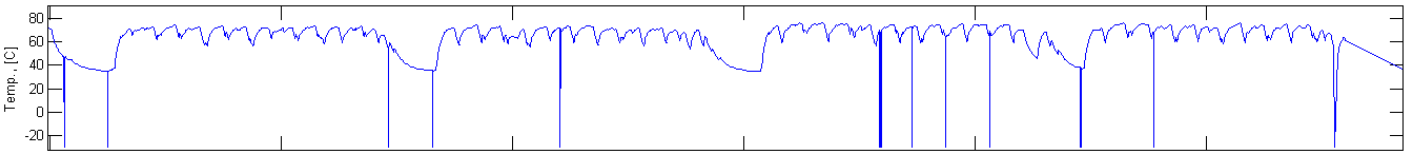
\includegraphics[width = \textwidth]{wykresy/ex_temp.PNG}
\caption{Example of~raw temperature data.}
\label{fig: ex_temp}
\end{figure}

In the~first step, the~outliers have been removed from the~data. In this case outliers are values lower than $0$. This effect in~the~signal is~considered to~be acquisition error since such values are forbidden by~the~physics of~the~process. Removed values have been replaced using local linear interpolation, which in~practice is~equivalent to~the~mean value of~the~neighboring samples (see Eq. \ref{eq:interp}).

\begin{equation}\label{eq:interp}
  x_{i}=\frac{x_{i-1}+x_{i+1}}{2} \quad \forall i: x_i<0
\end{equation}

The SCADA system that registered this data reacts to~the~value changing by~at~least predefined $\Delta T$, in~this case, equal to~1 degree Celsius. This approach allows reducing the~number of~recorded samples because repeating values are not stored. Linear interpolation is~the~simplest, yet best-suited method for interpolating such variables because, by~definition, the~intermediate sample can only take the~value between the~two existing neighbors. Unfortunately, the~described acquisition method makes the~data not evenly sampled, so after that, the~resampling was performed with output sampling period fixed to~15 minutes. To achieve that goal author used built-in Matlab function \code{resample}. 

After the~preprocessing, ICA was used to~separate the~intrinsic information sources in~the~dataset, which effectively allowed to~extract the~information indicating the~variation in~the~technical condition of~one of~the~gearboxes. In practice, four output variables are produced, that are called \emph{independent components} of~the~dataset. One of~those is~expected to~contain the~damage-indicating information. A~detailed description of~used ICA algorithm can be~found in~the~appendix in~section \ref{app_ica}.

When the~independent components are obtained, for each of~them algorithm searches for an~index $ind$ in~the~time domain that divides the~component into two parts that have the~highest possible difference in~the~mean value (see Eq. \ref{eq:divind}). 

\begin{equation}\label{eq:divind}
  ind=\argmaxB_i(\mathrm{abs}(\mathrm{mean}(x[1:i])-\mathrm{mean}(x[i+1:end])))
\end{equation}

Then, the~component characterized by~the~highest difference of~means is~identified as~the~component of~interest. Cross-correlating this component with all original channels allows determining which of~the~gearboxes the~misbehavior is~coming from. Correlation coefficients for this evaluation have been calculated using built-in Matlab function \code{corrcoef}. 


Finally, the~selected feature is~segmented into individual days based on~known sampling parameters. For each day, the~squared variance $vs^{(D)}$ is~calculated for each day $D=\{1,2,...,N\}$ where N is~the~number of~days in~the~data set. 

\begin{equation}\label{eq:divind2}
  vs^{(D)}=\left(\frac{1}{n}\sum^n_{i=1}\left(x_i^{(D)}-\mu^{(D)} \right)\right)^2,
\end{equation}
where $x^{(D)}$ is~segment of~a~particular day, $n$ is~its length and $\mu^{(D)}$ is~its mean value. 

Obtained vector $vs$ is~thresholded based on~its mean value $thr=mean(vs)$. The day where $vs>thr$ is~when the~overheating began. Functional flowchart of~the~procedure is~presented in~Figure \ref{fig: sch_ica}. The~procedure has been published in~\cite{wodecki2017application}.

\begin{figure}[ht!]
\centering

\includegraphics[width = 0.4\textwidth]{wykresy/sch_ica.png}
\caption{Flowchart of~proposed procedure.}
\label{fig: sch_ica}
\end{figure}

\subsection{Work regimes distinction using EM}\label{temp_em}

In this section the~methodology using the~clustering method was developed for the~long-term observations of~the~temperature in~order to~detect gearbox fault, that manifests itself as~a~non-typical behavior of~the~temperature data. The algorithm also identifies the~specific character of~the~work at~the~beginning and end of~the~week. For this methodology author analyzes temperature data acquired by~commercial, multichannel low-frequency data logger installed on~the~belt conveyor gearboxes in~a~copper ore mine.

Before starting any data analysis one should be~sure that the~data was acquired properly and the~incorrect values were removed, which allows to~avoid coming to~the~false conclusions of~the~analysis. The pre-processing procedures are obligatory in~case of~temperature data from belt conveyor gearbox. Author applied two-step procedure: data cleaning and resampling performed in~the~same way as~described in~section \ref{temp_ica}. The data after application of~pre-processing procedures is~shown in~Fig. \ref{fig: L222_55_data}.

\begin{figure}[ht!]
\centering
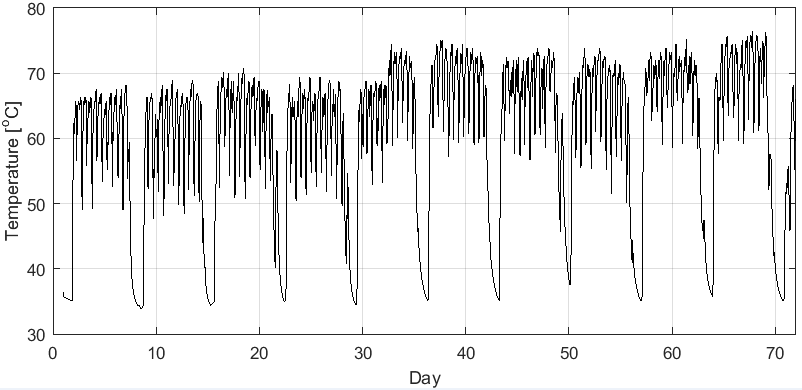
\includegraphics[width = 1\textwidth]{wykresy/L222_55_data.png}
\caption{Real temperature data from belt conveyor gearbox after pre-processing.}
\label{fig: L222_55_data}
\end{figure}

As one can see, visible cyclic drops of~the~temperature value are present. They are connected to~the~weekend periods when the~conveyor is~not operating. In that time the~gearbox is~cooled down to~the~ambient temperature. That specific behavior allows to~easily split the~data into segments corresponding to~each week of~the~belt conveyor operation. Moreover one can notice that at~$33$rd day of~collected data the~sudden increase in~the~temperature value occurs. Values of~temperature remain elevated for a~long time. The increase of~temperature is~a~symptom of~a~change of~technical condition of~a~machine. Therefore the~aim of~the~work is~to~propose an~anomaly detection procedure, which automatically indicates the~alarming time point.

Using the~time information, pre-processed data was segmented into sub-signals related to~one day of~a~belt conveyor operation. In Fig. \ref{fig: L222_55_days} one can see a~difference between the~behavior of~examined data depending on~the~day of~the~week. It should be~mentioned that in~the~copper ore mine there is~a~four shift work system. Moreover, on~Saturday the~work finishes at~6 p.m. and then begins at~6 a.m. on~Monday. Therefore, during the~$36$-hour stoppage in~operation, the~belt conveyor is~cooled down to~the~ambient temperature. This time period is~used for planned maintenance tasks. In other days the~cyclic breaks in~working are caused by~blasting procedures, which in~copper ore mine are performed twice during the~day. It is~reflected in~the~time series as~two temperature local minima about $9$ a.m. and $9$ p.m. Such behavior of~data can be~the~indicator in~the~clustering process, which is~used to~recognize working days when the~overheating takes place.

\begin{figure}[ht!]
\centering
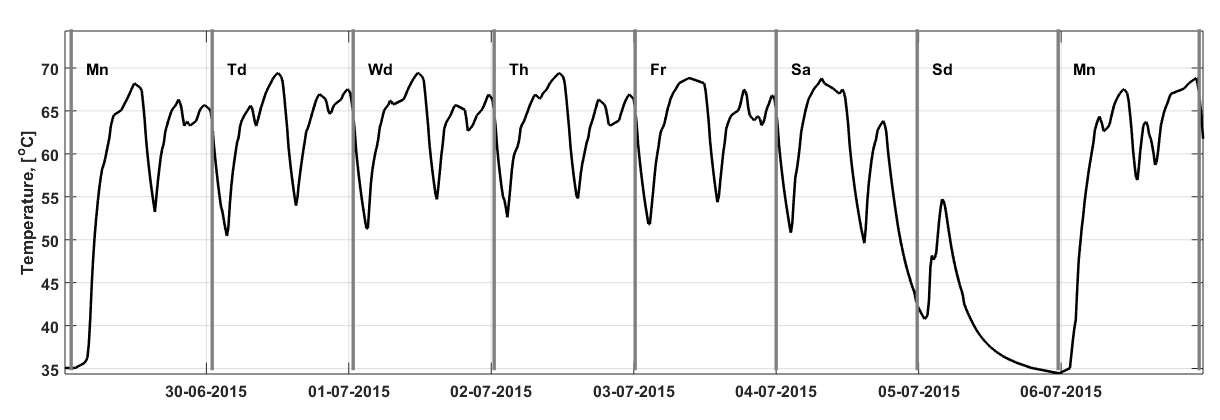
\includegraphics[width = \textwidth]{wykresy/days.png}
\caption{Behavior of~the~temperature time series depending on~day of~the~week.}
\label{fig: L222_55_days}
\end{figure}

The clustering procedure used for unsupervised anomaly detection is~the~Expectation-Maximization algorithm, described in~detail in~the~appendix in~section \ref{EM}. Statistics used to~feed the~clustering algorithm were simple, yet informative:

\begin{itemize}
\renewcommand{\labelitemi}{$\bullet$}
\item Maximum value of~the~day, 
\item Dispersion of~values of~the~day,
\item Value at~the~end of~the~day,
\end{itemize}
more formally:

\begin{equation}
  \chi=\left[\max(x), \max(x)-\min(x), x_{end} \right]
\end{equation}

The~three-dimensional feature vector of~described statistics has been constructed in~the~time domain for each day. Clustering of~this vector in~three dimensions using the~Expectation-Maximization algorithm (see section \ref{EM}) allowed to~classify the~days, and identify those revealing the~anomalous behavior. Functional flowchart of~the~procedure is~presented in~Figure \ref{fig: sch_em}. The~procedure has been published in~\cite{wodecki2018unsupervised}.

\begin{figure}[ht!]
\centering

\includegraphics[width = 0.4\textwidth]{wykresy/sch_em.png}
\caption{Flowchart of~proposed procedure.}
\label{fig: sch_em}
\end{figure}


\subsection{Time-time map analysis for LHD fault detection}\label{temp_bulgaria}

In this section, the~author addresses the~subject of~long-term analysis of~LHD's engine coolant temperature data in~order to~identify the~abnormal behavior, impossible to~be noticed having only short-term section of~the~data. 

Instantaneous value of~the~temperature is~influenced by~many factors, such as~workload, ambient temperature, restrictions in~heat exchange with the~air (e.g. when cooler is~close to~the~wall or is~plastered with mud), overall temporal efficiency of~the~cooling system, etc. It is~crucial to~understand that all of~the~factors can vary in~time. That amount of~varying parameters makes short-time temperature data analysis very difficult. As a~solution to~this problem author proposes to~perform a~long-term analysis, which allows reducing the influence of~fast-changing factors like varying workload during a~single work shift, temporary difficulties with heat exchange or variations of~ambient temperature. In such case, it~is~assumed that relevant temperature changes will be~connected mainly with the~technical condition of~the~machine.

Statistical approach used in~this methodology allows for looking at~the~data in~more aggregated way than only as~a~raw time series (see section \ref{prep}) \cite{sikora2012regime,wylomanska2014signal,azami2012improved,rathi2006seeing,wylomanska2012identify}. Proposed method considers work shifts as~integral parts of~data and investigates their kernel density estimate functions (see section \ref{param}). Work performed by~the~LHD is~mainly transport of~ore from the~mining face to~the~dumping point, so in~the~long run character of~this task is~mostly consistent. Hence, temperature distribution from shift to~shift should be~similar. However, in~case of~change of~technical condition of~the~machine (failure, repair and such) we expect a~significant change of~density function to~happen. This change can regard not only the~shift of~whole distribution function towards higher or lower values but the~change of~the~dispersion of~values as~well. To identify those changes the~author proposes to~define diagnostic parameters that are selected based on~the~observation of~data behavior. Parameters are expected to~reveal sudden changes in~the~data representation and ease of~their analysis will result in~a~very practical way of~health condition changes identification.

\subsubsection{Preprocessing}\label{prep}

LHD machines operate in~highly time-varying environmental conditions in~the~underground mine. Changing load and variability of~tasks lead to~different amounts of~data and its varying quality. Because of~those difficulties, the~proper selection of~data has to~be performed. The~important issue with the~original record is~a~substantial amount of~missing data points. Since the~approach is~shift-oriented, the~first task is~to~eliminate shifts that have too much data absent. First, the~author proposes to~visualize data in~3D space where temperature $T$ is~represented in~the~domain of~local time $t$ describing the~time during one work shift, and $\Theta$ that is~long-term time indicating consecutive work shifts. It can be~rewritten as:

\begin{equation}
  T=f(t,\Theta)
\end{equation}

To extract the~usable part of~data, the~amount of~empty values for each shift is~counted and placed in~a~vector. After that, the~distribution density function of~the~obtained vector is~calculated. 

\begin{equation}
  \hat{f}_h(x)=\frac{1}{nh}\sum_{i=1}^n K\left(\frac{x-x_i}{h}\right),
\end{equation}
where $x_i$ are random samples from an~unknown distribution, $n$ is~the~sample size, $K(\cdot)$ is~the~kernel function and $h$ is~the~bandwidth.


The density function has two major modes representing shifts with much data missing, and shifts with only a~small amount of~data missing. The~local minimum of~density function between those modes indicates the~threshold value above which shifts are disregarded. 

\subsubsection{Parameterization}\label{param}

After selecting the~appropriate set of~shifts from the~initial data, the~probability density estimate function of~every shift is~calculated \cite{bowman1997applied}. Vectors of~function values for each shift are arranged into a~matrix that forms so-called probability density map. The map itself in~some way reveals the~behavior that we were looking for, but on~the~small scale consecutive distributions are quite inconsistent and parameterization is~difficult at~this point. To achieve a~more useful character of~the~map, we regard it~to~be an~image, and smooth it~using two-dimensional convolution filter:

\begin{equation}
  \hat{T}=T\circ M,
\end{equation}
where $\hat{T}$ is~the~filtered map $T$, $\circ$ is~the~convolution operator and $M$ is~a~quasi-Gaussian kernel:

\begin{equation}
M=\frac{1}{81}*
\begin{bmatrix}
  1 & 2 & 3 & 2 & 1 \\
  2 & 4 & 6 & 4 & 2 \\
  3 & 6 & 9 & 6 & 3 \\
  2 & 4 & 6 & 4 & 2 \\
  1 & 2 & 3 & 2 & 1 \\
\end{bmatrix}
\end{equation}
where division by~81 means normalizing the~kernel by~the~total sum of~its fields \cite{arce2005nonlinear}. Values of~the~kernel were selected experimentally. The~ordinary two-dimensional moving average would smooth the~map way too much, so the~bell curve was chosen for better selectiveness after the~filtration. It causes the~nearest samples to~have a~greater impact on~the~center sample and further samples to~have a~lesser impact. In practice, this operation slightly smooths the~sharp spikes and improves the~consistency within the~regimes that we want to~distinguish apart. It also allows for calculated statistics described in~the~next chapter to~take more consistent form.

\subsubsection{Statistics and event description}

Parameterization of~shifts will require data samples, but since density map has been modified it~means that data itself is~not the~same anymore, so we can’t use original temperature data any longer. The easiest way to~obtain data samples from new distributions is~to~draw them from the~inverse empirical cumulative density function estimates $\hat{C}$ created by~numerical integration of~the~smoothed probability density map $\hat{T}$ \cite{devroye1986sample} such as:

\begin{equation}
  \hat{C}_{(i,j)}=\sum_{k=1}^j \hat{T}_{(i,k)}
\end{equation}

When samples are obtained for each shift, the~vector of~interquartile ranges has been calculated. Interquartile range (IQR) is~defined as~a~measure of~statistical dispersion, being equal to~the~difference between the~upper and lower quartiles, such as:

\begin{equation}
  IQR_i=\overline{\left(\hat{C}_i^+\right)_{(J/2+1:J)}}- \overline{\left(\hat{C}_i^+\right)_{(1:J/2)}}
\end{equation}
where $(\cdot)^+$ means vector sorted in~the~ascending order, $\overline{(\cdot)}$ is~a~median operator and $J$ is~the~length of~$\hat{C}_i^+$ vector.

The~second statistic is~a~vector of~locations of~probability density map maxima for shifts, and it~can be~calculated directly from the~map. Each statistic is~expected to~indicate the~changes in~data occurring with respect to~the~global time $\Theta$. To identify timestamps of~those change points, in~each statistic we find a~point that splits the~statistic into two parts of~the~highest difference in~mean. Obtained points are expected to~allow to~localize regime changes in~time. The~procedure has been published in~\cite{wodecki2016condition}.

\subsection{Anderson-Darling statistic map for failure detection}\label{temp_ad}

In this section, the~author proposes to~use long-term temperature data analysis for evaluating changes in~a~technical condition connected to~engine overheating in~LHD machines. This method focuses on~developing an~alternative technique to~differentiate time segments containing data that describe different technical condition of~the~machine. Author takes advantage of~the~fact that the~statistical distribution of~temperature data differs according to~technical condition \cite{wodecki2016condition}. Appropriate transformation of~long-term temperature data and application of~Anderson–Darling (AD) statistic (see section \ref{met_ad}) allows quantifying those differences in~the~form of~a~two-dimensional map of~the~test statistic. Analysis of~this map results in~the~detection of~points where the~technical condition of~the~machine changes significantly.

Proposed method is~based on~long-term data observation. Based on~the~general assumption about the~way that overheating leads to~machine failure one can define three disjoint processes occurring consecutively:

\begin{itemize}
  \item[$\bullet$] \emph{Process 1:} Machine is~operating while in~bad technical condition, overheating significantly;
  \item[$\bullet$] \emph{Process 2:} Machine experiences a~cooling system failure, but is~still being operated;
  \item[$\bullet$] \emph{Process 3:} Failure is~repaired and machine operates in~good technical condition.
\end{itemize}

In such case one can describe those processes in~terms of~signal parameters:

\begin{itemize}
  \item[$\bullet$] \emph{Process 1:} High median, low variance (warning state approaching failure);
  \item[$\bullet$] \emph{Process 2:} High median, high variance (failure state);
  \item[$\bullet$] \emph{Process 3:} Low median, high variance (healthy state).
\end{itemize}

Despite the~relatively simple definition of~the~processes, it~is~not easy to~define one simple diagnostic criterion.

\subsubsection{Pre-processing}

Input data is~imported in~the~time domain, so pre-processing is~required. Firstly, non-overlapping six-hour segments of~the~signal that denotes six-hour work shifts, are framed into the~new matrix as~its columns. Then columns with an~excessive amount of~missing values are rejected based on~the~distribution of~their amount in~each column. Since remaining columns still contain small amounts of~missing values, they are interpolated using the~nearest-neighbour method. Such a~matrix representing the~temperature in~a~time-time domain is~ready for further analysis.

\subsubsection{Anderson-Darling statistic}\label{met_ad}

Because of~different behavior in~observed regimes (changing the~median and variance) the~author proposes to~calculate the~empirical cumulative distribution functions (ECDF) of~each work shift and compare statistic based on~distances between them. ECDF of~the~random variable $X$ can be~defined as:

\begin{equation}
  \hat{F}_n(t)=\frac{1}{n}\sum_{i=1}^n 1_{X_i\leq t}
\end{equation}
where $1_A$ is~the~indicator of~event $A$ and $n$ is~the~length of~realization of~$X$. 

Usually it~is~calculated in~supremum (Kolmogorov - Smirnov \cite{massey1951kolmogorov}) or quadratic (Cram{\'e}r - von Mises family \cite{laio2004cramer}) norm. For signal parameterization author proposes to~use statistic based on~quadratic norm between two ECDFs. Kolmogorov - Smirnov test is~widely recognized and used as~a~classical method, but AD test is~described in~the~literature as~more powerful and hence superior \cite{razali2011power,engmann2011comparing}. a~class of~measures of~discrepancy is~given by~Cram{\'e}r - von Mises family:

\begin{equation}
\label{one-sample_ad}
  Q^2=n \int\limits_{-\infty}^{\infty} \{F_n(x) - F(x) \}^2 \psi(x)dF(x)
\end{equation}
where $F_n(x)$ is~ECDF, $F(x)$ is~theoretical CDF that $F_n(x)$ is~compared to, $\psi(x)$ is~a~function of~weights. $\psi(x)=1$ gives $\omega^2$ statistic of~Cram{\'e}r - von Mises. To obtain Anderson - Darling statistic $A^2$ the~vector of~weights is~given by~$\psi(x)=[F(x)(1-F(x))]^{-1}$ \cite{pettitt1976two,cizek2005statistical}. In the~real data analysis the~integral in~formula \ref{two-sample_ad} reduces to~the~finite sum which corresponds to~the~distance between theoretical and empirical cumulative distribution functions in~appropriate norm.

In presented case author used two-sample Anderson - Darling statistic which is~modification of~(\ref{one-sample_ad}):

\begin{equation}
\label{two-sample_ad}
  A^2_{nm}=\frac{mn}{N} \int\limits_{-\infty}^{\infty} \frac{\{F^i_m(x) - F^j_n(x) \}^2} {H_N(x)(1-H_N(x))}dH_N(x),
\end{equation}
where $F^i_m$, $F^j_n$ are ECDFs of~$i^{th}$ and $j^{th}$ work shifts and $H_N$ with $N=n+m$ is~the~weight function, for $n$ and $m$ being the~number of~observations in~work shifts. The $H_N$ function is~given by~combining $F^i_m$ and $F^j_n$ distribution: $H_N(x)=\frac{mF^i_m(x)+nF^j_n(x)}{N}$. It is~used to~test hypothesis $F^i_m=F^j_n$. In presented method author calculates Anderson - Darling statistic defined by~(\ref{two-sample_ad}) for every pair of~shifts and construct 2D map of~values. The resulting map is~symmetric relative to~its main diagonal.

\subsubsection{Smoothing of~AD map}

After calculating the~map of~AD statistic, it~requires minor smoothing to~obtain more consistent levels in~distinctive areas of~the~map \cite{bowman1997applied}. The~author proposes to~use two-dimensional a~convolution-based filter with normalized triangular kernel \emph{K} based on~a~vector $v=\left[1,2,1 \right]$ (\ref{eq:kernel}). 
\begin{equation}
\label{eq:kernel}
K = \frac{v^T v}{\sum{\left(v^T v \right)}} = \frac{1}{\sum{\left(v^T v \right)}}\left[\begin{array}{ccc}1&2&1\\2&4&2\\1&2&1\end{array}\right] =
\left[\begin{array}{ccc}0.0625&0.125&0.0625\\0.125&0.25&0.125\\0.0625&0.125&0.0625\end{array}\right]
\end{equation}

\subsubsection{AD map analysis}

Considering knowledge about general behavior of~the~processes described in~previous sections, one can make a~few assumptions about the~expected structure of~AD map (see Fig. \ref{fig:map}):
\begin{enumerate}
\item ECDFs of~shifts within a~single process will be~similar, hence values of~AD statistic in~the~areas (1,1), (2,2) and (3,3) will be~relatively low, because those are the~areas where shifts of~a~given process are compared with shifts of~the~same process. 
\item ECDFs of~shifts from warning and failure processes are similar for failure shifts where the~machine was not cooled down on~purpose, and different for failure shifts where the~machine was purposely cooled down (regions (1,2) and (2,1)).
\item Analogous case occurs when comparing ECDFs of~shifts from failure and healthy process: they are similar for failure shifts where the~machine was purposely cooled down, and dissimilar otherwise (regions (2,3) and (3,2)).
\item Comparing warning and healthy processes, ECDFs are not similar at~all, hence those regions of~AD map will be~characterized with high values (regions (1,3) and (3,1)).
\end{enumerate}

\begin{figure}[ht!]
\centering
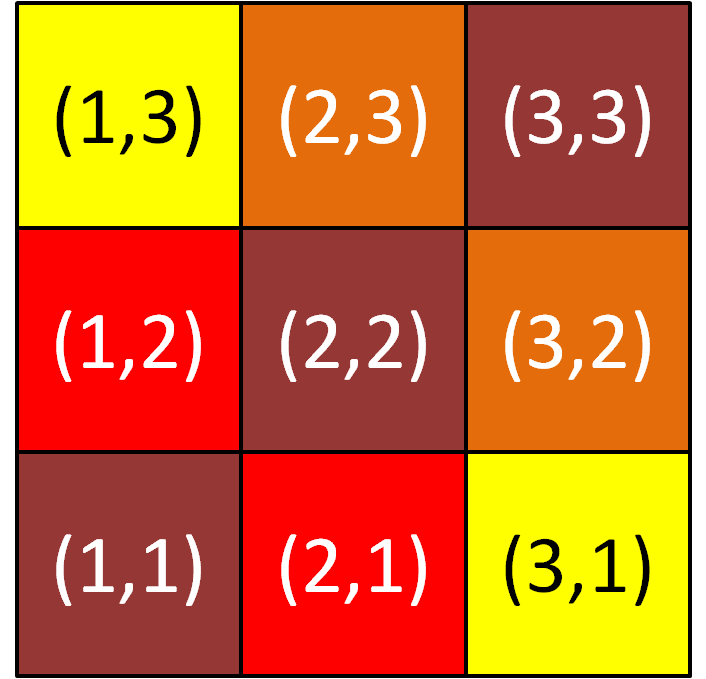
\includegraphics[width=0.5\textwidth]{wykresy/map.png}
\caption{Logical chart of~expected AD map}
\label{fig:map}
\end{figure}

It is~hard to~find transition points based on~two-dimensional data. Hence, the~author proposes to~determine the~threshold based on~one-dimensional statistic. Taking advantage of~previously mentioned assumptions, it~is~expected that the~variance of~AD map vectors will vary according to~the~area. Hence, in~a~next step one-dimensional sample variance of~the~smoothed map is~calculated. Since the~second process shares similar features with two remaining ones, which on~the~other hand are different from each other, one can expect certain behavior of~the~variance values of~particular groups of~AD map columns:

\begin{itemize}
\item[$\bullet$] \textbf{Group regarding process 1 (columns of~areas (1,x)):} relatively high variance values. AD statistic values will be~low when comparing process 1 to~itself, medium when comparing it~to~process 2 (similar median) and high when comparing it~to~process 3 (no similar parameters);
\item[$\bullet$] \textbf{Group regarding process 2 (columns of~areas (2,x)):} relatively low variance values. AD statistic values will be~low when comparing process 2 to~itself, and medium when comparing it~to~processes 1 and 3 (similar median or variance);
\item[$\bullet$] \textbf{Group regarding process 3 (columns of~areas (3,x)):} relatively high variance values. AD statistic values will be~low when comparing process 3 to~itself, medium when comparing it~to~process 2 (similar variance) and high when comparing it~to~process 1 (no similar parameters);
\end{itemize}

Based on~that assumption one could imagine that group 2 is~expected to~exhibit lower sample variance than groups 1 and 3. Hence, it~is~proposed to~threshold sample variance vector based on~the~histogram with bin width $BW$ calculated using Freedman-Diaconis rule defined as~\cite{freedman1981}:

\begin{equation}
  BW=2\frac{IQR(X)}{\sqrt[3]{n}},
\end{equation}
where $n$ is~a~number of~elements in~the~vector $X$.

Values describing group 2 are expected to~cluster around lower variance value than values describing groups 1 and 3, so a~natural local minimum is~expected to~appear on~the~histogram between group 2 and groups 1 and 3. Location of~that local minimum serves as~a~threshold that allows to~separate groups using the~variance vector as~a~feature, and hence to~find the~transition points between technical condition states. The~procedure has been published in~\cite{wodecki2017technical}.

\section{Muiltichannel spectrogram analysis using PCA}\label{met_pca}

A multichannel vibration data processing method in~the~context of~local damage detection in~gearboxes is~presented in~this section. The purpose of~the~approach is~to~achieve more reliable information about local damage when using several channels in~comparison to~results obtained for single-channel vibration signal. 

First, the~transformation of~$N$ input channels into time-frequency representations is~performed. For this purpose, a~spectrogram is~used according to~the~definition provided in~the~appendix (see section \ref{STFT}). As a~result, a~three-dimensional data structure is~created, such that:

\begin{equation}
  S^{(i\times M\times K)}=spec\left(X_i^{(1\times L)} \right),
\end{equation}
where $i=(1,\dots,N)$ is~the~number of~input channel, $L$ is~the~number of~samples in~each input channel, and $M\times K$ is~the~size of~calculated spectrograms in~frequency and time domain respectively.

In the~next step, the~time-frequency maps are divided into narrow-band slices corresponding to~given frequency bins. As a~result obtained structure can be~rearranged to~serve as~$N-$dimensional sub-signals for each frequency band since $N$ channels are analyzed. Then PCA is~applied to~$N-$dimensional sub-signals (see section \ref{app_pca}), that provides the~set of~$N$ principal components related to~the~analyzed subsignal. The~formal definition of~this operation can be~written as:

\begin{equation}
  PC^{(N\times j\times K)}=PCA\left(S^{(N\times j\times K)} \right),
\end{equation}
where $j=(1,\dots,M)$ indicates subsets related to~individual frequency bins, 


From among those, the~first principal component is~selected and arranged into the~new matrix of~the~same dimensions as~the~original spectrograms, which in~practice stands for $PC^{(1\times M\times K)}$. As a~result, new time-frequency map is~obtained, which is~made of~selected principal component vectors corresponding to~given frequency bands. At the~end, the~newly constructed time-frequency map is~aggregated in~the~time domain to~produce one-dimensional time series which is~expected to~contain cyclic impulsive components connected to~local damage. Flowchart of~the~proposed procedure is~presented in~Fig. \ref{fig: pca_block}. The~procedure has been published in~\cite{wodecki2016combination}.

\begin{figure}[ht!]
\centering
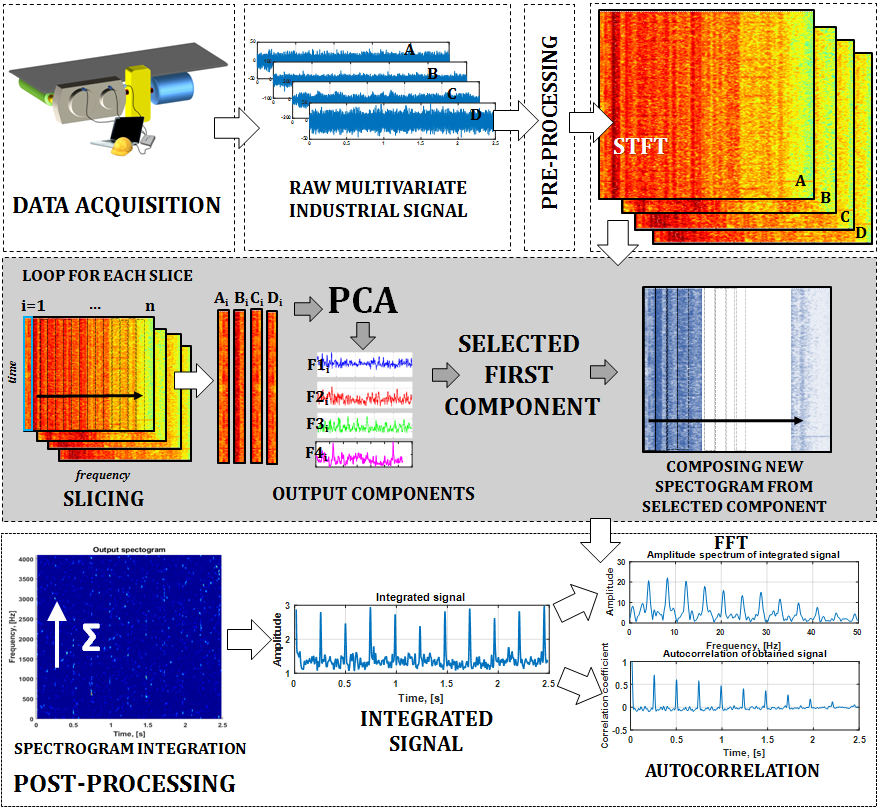
\includegraphics[width = \textwidth]{wykresy/pca_block.png}
\caption{Functional schematic of~presented method.}
\label{fig: pca_block}
\end{figure}


\newpage
\section{Methods for multidimensional domain analysis using NMF algorithms}

In this section, the~author describes techniques developed based on~the~factorization of~multidimensional data representations. In all described cases vibration signals are analyzed. From among many different multidimensional data representations two have been selected because of~their properties: spectrogram, which is~a~squared magnitude of~Short-Time Fourier Transform (STFT) and Cyclic Spectral Coherence (CSC). A~spectrogram is~a~time-frequency representation, and it~can be~interpreted in~two ways: either as~a~short-time Fourier spectrum that changes in~time or as~time-domain subsignals described in~narrow frequency bands within the~entire frequency spectrum of~the~input signal. CSC is~a~bi-frequency representation with two frequency axes describing nonlinear links between the~carrier frequency and modulating frequency. It can be~interpreted as~autocorrelation of~spectrogram matrix and provides information about cyclic modulations with respect to~the~carrier frequency domain.

General idea of~matrix factorization assumes that it~is~possible to~approximate a~matrix with two (or more) factors being (typically) lower-rank matrices (see Figure \ref{fig:met_nmf}). There is~a~lot of~different classes of~factorization algorithms, the~most popular being: Singular Value Decomposition (SVD) \cite{cempel2007multidimensional,cempel2008generalized}, Eigenvalue Decomposition (EVD) \cite{golub2012matrix,johnson1985matrix}, LU decomposition \cite{householder2013theory}, Cholesky decomposition \cite{golub2012matrix,johnson1985matrix} etc.

\begin{figure}[ht!]
\centering

\includegraphics[width=0.8\textwidth]{wykresy/met_nmf.png}
\caption{General idea of~matrix factorization}
\label{fig:met_nmf}
\end{figure}

Each class of~algorithms can be~characterized with different properties, e.g. some only accept and return square matrices, others also produce third diagonal matrix, etc. NMF-type algorithms, on~the~other hand, have the~unique property of~only accepting and returning matrices with nonnegative entries. 


\subsection{STFT analysis taking advantage of~NMF encoding matrix}\label{met_nmf_enc}

In the~first case of~NMF-based method design author focuses on~the~utilization of~\emph{encoding matrix} (matrix H in~Figure \ref{fig:met_nmf}) generated by~NMF algorithm while factorizing spectrogram matrix of~vibration signal recorded on~the~damaged bearing of~the~belt conveyor's drive pulley. Flowchart of~the~described procedure is~presented in~Fig. \ref{fig:met_enc_nmf}.

In the~first step spectrogram matrix of~the~signal is~calculated according to~the~description in~section \ref{STFT} in~the~appendix. Then author used Semi-Binary NMF (see section \ref{ap_sbnmf} in~the~appendix) algorithm to~group spectra vectors across all timestamps of~the~spectrogram. Encoding matrix produced by~NMF carries information about the~timestamp occurrence within clusters, which allows constructing so-called “partial output spectrograms”. They are matrices of~zeros with appropriate spectra vectors distributed among them. As a~result of~this step, we obtain $J$ partial spectrograms where $J$ is~a~predefined number of~clusters. The inverse short-time Fourier transform (ISTFT) is~performed on~all of~them using built-in Matlab function \code{istft} \cite{benesty2007springer}, and the~one of~maximum kurtosis is~selected for further processing.

At this point obtained selected signal reveals presence at~correct timestamps of~impulses occurrence, but those areas do not look like impulses yet. To extract the~correct form of~the~impulses, highpass filtration is~required. It gets rid of~low-frequency high-energy frequency components and preserves impulse present in~a~wide band of~the~spectrum. The~procedure has been published in~\cite{wodecki2017local}.


\begin{figure}[ht!]
\centering

\includegraphics[width=.4\textwidth]{wykresy/met_enc_nmf.png}
\caption{Flowchart of~the~proposed procedure}
\label{fig:met_enc_nmf}
\end{figure}

\subsection{STFT analysis taking advantage of~NMF base matrix}\label{met_nmf_base}

In the~next case of~NMF-based method design author utilizes so-called \emph{base matrix} (matrix W in~Figure \ref{fig:met_nmf}) generated by~NMF algorithm while factorizing spectrogram matrix of~vibration signal recorded on~the~damaged bearing of~the~copper ore crusher. In that case base matrix produced by~NMF was used to~classify spectra vectors along the~time dimension. As a~result, the~filter characteristic is~designed, that allows isolating the~damage component. Flowchart of~the~described procedure is~presented in~Fig. \ref{fig:met_base_nmf}.

Firstly, the~signal has to~be transformed into a~time-frequency domain. For such transformation spectrogram has been chosen (see section \ref{STFT}). Considering it~as~nonnegative data matrix author applies NMF to~factorize spectrogram. In this context NMF is~used as~clustering tool group spectra vectors $\textrm{Spec}[f,\Delta t[i]]$, where $f$ denotes full Nyquist frequency domain for given data. Obtained spectrogram matrix $Spec$ will serve as~input matrix $\mathbf{V}$ for NMF factorization (see Eq. \ref{V1}). To perform the~factorization, the~author defines the~value $r$ as~the~rank of~factorization. Then NMF factorization is~performed to~obtain the~matrix \textbf{W} that will be~composed of~\textit{r} vectors - related to~clusters - that contain description of~spectral content of~each cluster $i=1 \dots r$. Each column vector of~\textbf{W} is~considered to~be averaged spectral density and can be~used as~filter characteristic (also named \emph{selector}).

Finally, the~input signal is~filtered with FIR filter, where the~given selector is~used as~filter frequency response \cite{alan1989discrete}. In~the~end, envelope spectra of~obtained signals are calculated to~inspect fundamental and harmonic frequencies of~the~components \cite{randall2011rolling}. Additionally, IFB can be~presented as~a~frequency band for which the~desired selector is~the~strongest of~the~whole bank. The~procedure has been published in~\cite{wodecki2017novel}.

\begin{figure}[ht!]
\centering

\includegraphics[width=.4\textwidth]{wykresy/met_base_nmf.png}
\caption{Flowchart of~the~proposed procedure}
\label{fig:met_base_nmf}
\end{figure}

\subsection{CSC analysis taking advantage of~complete NMF output}\label{met_nmf_both}

In this chapter author presents multistage processing methodology for fault identification in~rotating machinery scenario, however, it~is~suitable for the~case when the~other periodic impulsive component is~also present in~the~signal. The~flowchart in~Figure \ref{fig:met_mcnmf} presents the~outline of~the~proposed procedure.

\begin{figure}[ht!]
\centering
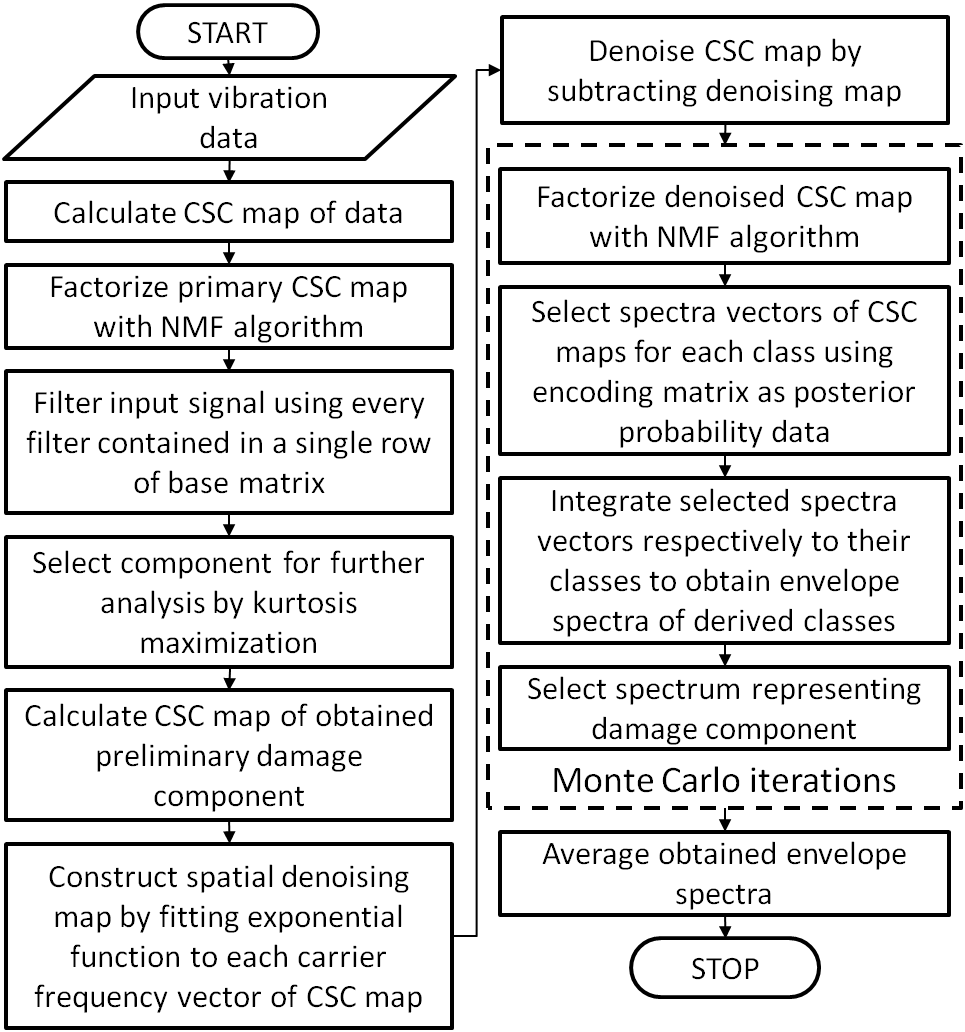
\includegraphics[width=.7\textwidth]{wykresy/met_mcnmf.png}
\caption{Flowchart of~the~proposed procedure}
\label{fig:met_mcnmf}
\end{figure}

The main idea is~focused on~utilizing all the~information that the~factorization algorithm can provide for such a~problem. Typically when NMF is~used, authors of~proposed methods are only interested in~the~information held by~one of~the~output matrices. One of~the~typical examples is~time-frequency map analysis \cite{wodecki2017local}, where authors use \emph{encoding matrix} to~classify spectra vectors in~the~time domain, allowing to~extract impulses from vibration data. While the~method is~effective, it~is~important to~note that the~\emph{base matrix} remains unused, leaving behind the~information that can still be~of~some value. Based on~this idea, the~author proposes to~utilize the~information from both output matrices in~a~sequential manner. 

Since the~input vibration signal has a~relatively complex structure in~terms of~the~presence of~cyclic components, instead of~time-frequency representation author decided to~use the~bi-frequency representation called Cyclic Spectral Coherence (CSC) as~a~basis for the~analysis (see section~\ref{app_csc} in~the~appendix). In the~first stage of~processing, CSC map is~firstly factorized with NMF algorithm (see section~\ref{app_nmf} in~the~appendix), and the~base matrix is~used as~a~set of~filters in~the~carrier frequency domain. Then, the~input signal is~filtered through a~selected filter, which results in~significant improvement of~the~signal in~terms of~SOI detectability \cite{wodecki2017novel}. 

In the~second stage of~processing obtained signal is~spatially denoised in~the~bi-frequency domain. In order to~achieve that, every vector of~full modulating frequency range within a~single carrier frequency bin is~modeled with a~decaying exponential function. This way it~is~possible to~construct a~spatial noise model in~the~form of~a~matrix with the~same dimensions as~the~CSC matrix. After subtracting noise model matrix from the~CSC map, the~latter becomes more clear and visibility of~damage-related frequency components is~improved.

In the~third stage, denoised CSC map is~again factorized with NMF algorithm within the~iterations of~Monte Carlo (MC) simulation \cite{metropolis1987beginning}. In each iteration damage-related envelope spectrum is~extracted, and after averaging final form of~the~envelope spectrum is~obtained.

\subsubsection{Multidimensional approach}

Analytical procedures incorporating various types of~multidimensional analysis very often focus on~features regarding only one of~the~dimensions of~considered data. Examples of~such approach contain e.g. frequency dimension of~spectrogram matrix (spectral selectors, spectral kurtosis~\cite{antoni2006spectral}), time dimension of~spectrogram matrix (cyclic impulses detection~\cite{kruczek2017cyclic}), modulation frequency domain of~bi-frequency map (fault frequency indication~\cite{kruczek2017multiple}) etc. 

In contrast to~such approach presented method takes advantage of~information extracted with respect to~both dimensions of~the~two-dimensional map being the~key subject of~analysis. In the~first stage, a~filter is~constructed based on~base matrix carrying information about the~carrier spectrum. The filter allows extracting one cyclic component from the~mixture of~two. In the~third stage, encoding matrix is~analyzed in~order to~obtain the~enhanced representation of~the~envelope spectrum of~the~fault component, that after post-processing reveals the~perfectly clean spectral structure of~the~fault.

\subsubsection{Spatial noise modeling}\label{denoise}

In order to~enhance the~efficiency of~NMF operation in~the~third stage of~analysis, quality of~the~CSC map can be~improved. To achieve this, the~author decided to~introduce preconditioning as~a~second step of~the~analysis. Noise levels across the~map are spatially modeled and subtracted from the~data for each $\Delta f$. 

The spatial context is~created by~analysis of~each carrier frequency bin $f = \left[f_1, \dots ,f_m \right]$ along the~modulating frequency dimension $\alpha = \left[\alpha_1, \dots ,\alpha_n \right]$. Each vector is~modeled specifically to~describe the~energy of~the~noise within this frequency band. However, to~avoid improper fitting, samples of~impulses are treated as~outliers among the~general shape of~decaying noise and rejected based on~data distribution. 

Denote single modulation vector from CSC map as~$C_i=\left|\hat{\gamma}_X(f_i,\alpha)\right|^{2}$ where $i \in 1, \dots, m$ and $\alpha = \left[\alpha_1, \dots ,\alpha_n \right]$. Author proposes to~define outlier cutoff threshold as~$99^{th}$ percentile for $C_i$ denoted as~$\hat{c}_{99}$ and defined as:

\begin{equation}
  P\left( C_i\leq\hat{c}_{99} \right)\geq 0.99.
\end{equation}

In such case it~is~possible to~exclude indices of~values higher than $\hat{c}_{99}$ from the~domain $\alpha$ and denote such modified domain of~$\alpha$ as~$\alpha_{mod}$, and respective background noise reference data originating from $\left|\hat{\gamma}_X(f_i,\alpha)\right|^{2}$ as~$\left|\hat{\gamma}_X(f_i,\alpha_{mod})\right|^{2}$ where $i \in 1, \dots, m$.

Considering described modeling conditions, each vector $\left|\hat{\gamma}_X(f_i,\alpha_{mod})\right|^{2}$ is~modeled with single-term exponential function using non-linear least squares method. Obtained parameters $a_i \in A$ and $b_i \in B$ (where $A$ and $B$ are vectors of~parameters for entire $f$ domain) of~exponential function allow then to~obtain the~noise model over a~modified domain $\alpha_{mod}$ for given $f_i$. Such modeled noise components are arranged into a~spatial noise map $N$ defined as~follows:

\begin{equation}
  N(i,\alpha_{mod})=a_i \exp \left( b_i \left|\hat{\gamma}_X(f_i,\alpha_{mod})\right|^{2}\right),
\end{equation}
that can be~subtracted from the~CSC map, effectively causing its denoising:

\begin{equation}
  \mathrm{CSC_d}= \left|\hat{\gamma}_X(f,\alpha)\right|^{2}-N,
\end{equation}
where $\mathrm{CSC_d}$ denotes denoised CSC map.
%  \newpage

% \begin{figure}[ht!]
% \centering
% 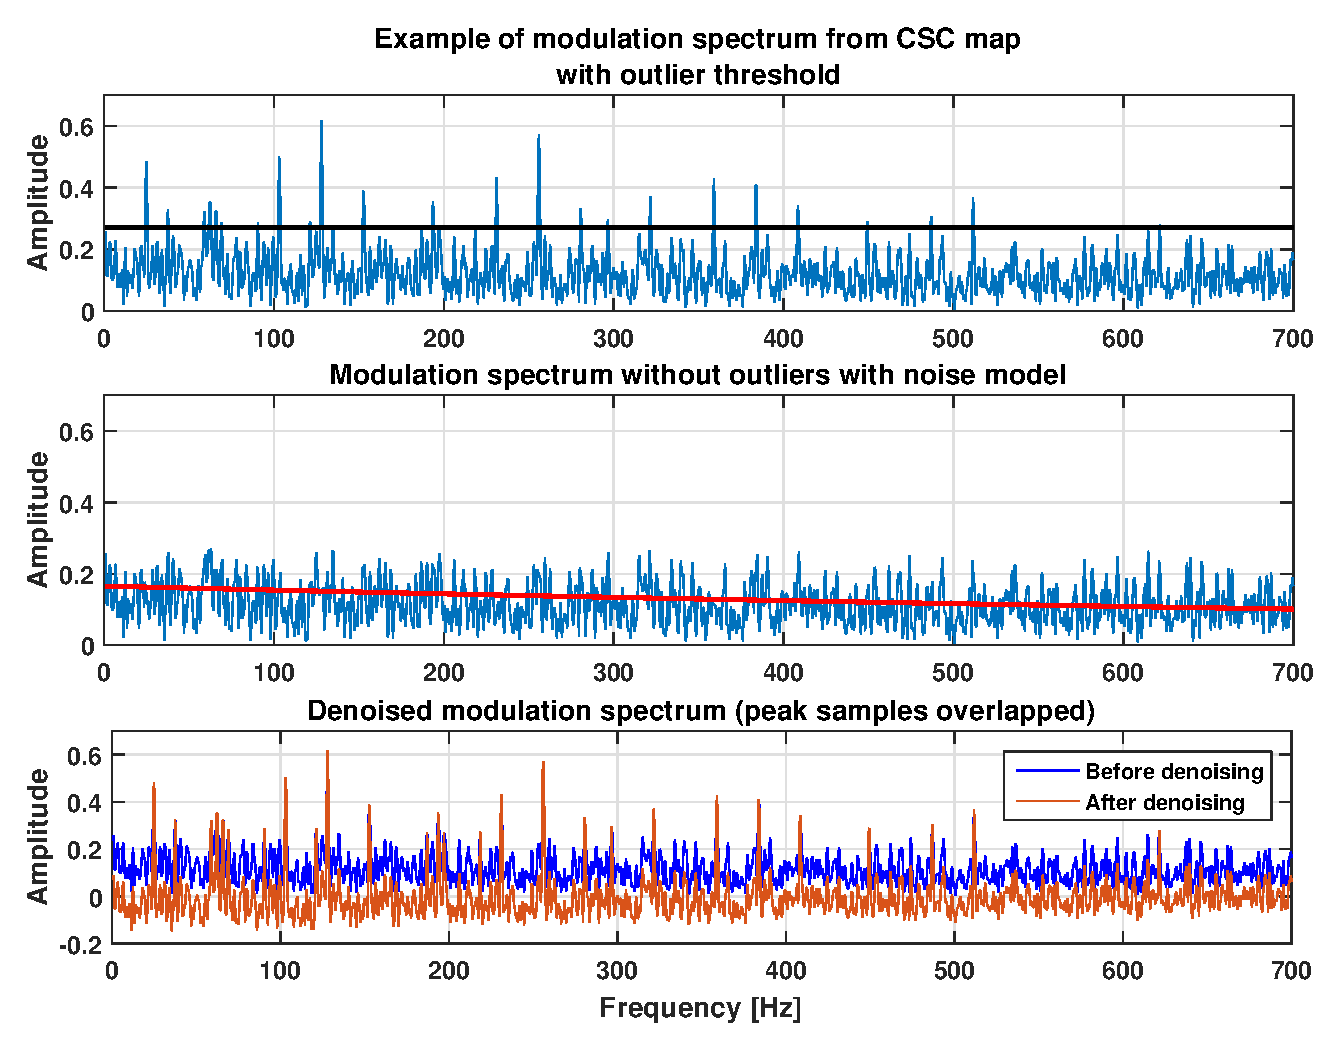
\includegraphics[width=.8\textwidth]{wykresy/ex}
% \caption{Example of~spatial denoising}
% \label{fig:ex}
% \end{figure}

\subsubsection{Monte Carlo simulation}\label{mcmc}

Monte Carlo (MC) methods are a~class of~algorithms that utilize random sampling in~numerical computation problems (see section \ref{app_monte}) \cite{metropolis1987beginning, metropolis1949monte}. The main idea is~to~use large-scale randomness to~discover deterministic behavior in~the~regarded problem. By the~law of~large numbers, the~expected value of~a~random variable can be~obtained approximately by~averaging independent samples of~the~variable using i.e. mean, median, etc. 

In the~presented application MC simulation is~used to~obtain good-quality envelope spectrum of~damage component in~the~diagnostic signal. In practice, the~role of~random sampling is~played by~calculating randomly initialized NMF of~denoised CSC map, using the~information provided by~obtained encoding matrix, and based on~that extracting envelope spectrum related to~local damage. Such spectrum will not be~exactly the~same in~every MC iteration, however, it~is~expected that most of~the~time outcome will be~mostly correct. Finally, averaging of~obtained results is~expected to~reveal true envelope spectrum related to~damage by~getting rid of~uncommon frequency components.

Within the~MC iterations, NMF is~used to~distinguish the~predefined amount of~groups $k$ of~different behavior to~be found in~denoised CSC map. Those groups are here called classes. As mentioned before, one of~them is~expected to~carry information about the~informative component related to~local damage. For the~interpretation of~obtained classes, the~author takes advantage of~the~encoding matrix operating in~the~domain of~modulating frequency. It is~easiest to~visualize this operation as~using posterior probability data (class indicator data) produced by~a~clustering algorithm. Encoding matrix can be~interpreted as~carrying information which class given point (here - given frequency component as~entire spectrum vector in~the~carrier domain integrated to~a~single value in~the~modulation domain) belongs to. Using this information it~is~possible to~construct the~envelope spectrum for each class. At this point, it~is~important to~be able to~automatically select the~cluster of~interest. It is~done by~calculating the~kurtosis value of~the~envelope spectrum vector for each class and selecting class with the~highest value. It is~motivated by~the~fact, that spectrum of~this class is~expected to~contain a~small number of~different frequency components, with the~majority of~zero values, while other classes will be~populated much more densely with frequency components carrying more coherent values of~energy. In this context, kurtosis value is~expected to~be highest for the~class related to~damage.

Finally, the~entire set of~envelope spectra obtained from MC iterations has to~be averaged to~obtain the~final result. Typically it~is~done using the~ordinary sample mean, however in~this application such an~approach would be~disadvantageous. Due to~random initialization of~NMF, in~most cases selected classes of~envelope spectra are expected to~contain a~small number of~improper frequency components in~the~notion of~false-positive result or, on~the~other hand, to~have expected correct frequency components missing. After using the~sample mean to~the~average large amount of~obtained spectra, those impurities of~the~first type (false-positives) will remain as~small values contaminating the~desired perfect spectrum after averaging. To avoid this effect, the~author used the~median function for averaging the~spectra. This way, unwanted contaminants will be~omitted, instead of~reduced.

As a~summary of~this section, single MC iteration is~constructed as~follows:

\begin{itemize}
  \item[$\bullet$] Factorize denoised CSC map with NMF;
  \item[$\bullet$] Use encoding matrix as~indicator data to~assign spectra vectors to~their respective classes;
  \item[$\bullet$] Integrate spectra vectors within each class placing them at~correct positions with respect to~the~modulating frequencies they stand for, which forms envelope spectra for all classes;
  \item[$\bullet$] Select class representing component of~interest.
\end{itemize}

\subsubsection{Kurtosis as~criterion for cluster selection}

In the~described application for every MC iteration, it~is~imperative to~be able to~automatically identify vector loosely populated with high-value nonuniform samples (highly non-Gaussian distribution) from among other vectors populated more densely with a~larger amount of~similar values (closer to~Gaussian distribution). In such context it~is~a~reasonable idea to~select vector with the~highest value of~kurtosis, which is~defined as~follows:

\begin{equation}
\label{eq:kurtosis}
Kurt[X]=\frac{m_4}{{m_2}^2}=\frac{\frac{1}{n} \sum_{i=1}^{n} \left(x_i - \overline{x} \right)^4}{\left({\frac{1}{n} \sum_{i=1}^{n} \left(x_i - \overline{x} \right)^2}\right)^2}
\end{equation}
where $m_4$ is~the~fourth sample central moment and $m_2$ is~the~second sample central moment (sample variance). The~procedure has been published in~\cite{wodecki2019impulsive}.


\newpage
\section{Automatic information extraction with Progressive Genetic Algorithm}\label{met_pga}

In this section author proposes novel method for vibration data analysis measured on~the~rolling bearing. In presented solution author pursues the~approach of~determining informative frequency band (IFB) of~the~signal, and hence extracting information about the~presence of~damage, that is~based on~optimal filtration. In practice, a~filter is~found, that is~dedicated to~optimally process the~given data. In opposition to~using classic adaptive filters \cite{makowski2014new,makowski2013procedure} or designing optimal filter prior to~predefined specification \cite{nilsson2003digital}, presented approach is~fully data-driven, and fitness function evaluates the~solutions only in~terms of~filtration performance. This way no functional constraints are imposed on~the~way that filter is~constructed by~the~evolution process. 

From mathematical point of~view, filter is~just an~equation of~discrete transfer function with $N$ coefficients (see eq. \ref{eq:fir}). For optimal filtering, both the~value of~$N$ and coefficients values should be~found. From such perspective, diagnostic methodology can be~considered as~multidimensional optimization problem. Genetic Algorithm (GA) is~one of~the~most frequently used tool for such task. However, it~should be~noted that presented procedure is~not a~simple application of~GA to~filter design. Author proposed a~complete progressive procedure for data-driven arbitrary filter development having no prior requirements. Kurtosis of~filtered signal is~used as~an~fitness value in~the~objective function, since local damage in~rotating machines presents itself as~wideband impulses in~vibration signal. However, an~original concept of~termination procedure is~proposed. In this work, progressive genetic algorithm has been applied for the~design of~linear phase digital FIR filter. Details of~ordinary GA operation can be~found in~the~appendix in~section \ref{GA}. The~procedure has been published in~\cite{wodecki2018optimal}.

\subsubsection{Filter encoding}

A~filter is~a~frequency selective object that allows a~certain frequency to~pass while attenuating the~others. Traditionally, different techniques exist for the~design of~digital filters. Of these, the~windowing method is~the~most popular \cite{alan1989discrete}. In this method, the~ideal impulse response is~multiplied with a~window function. There are various kinds of~window functions (Butterworth, Chebyshev, Kaiser, etc.), depending on~the~requirements of~ripples on~the~passband and stopband, stopband attenuation and the~transition width. These various windows limit the~infinite length impulse response of~ideal filter into a~finite window to~design an~actual response. However, windowing methods do not allow to~sufficient control of~the~frequency response in~the~various frequency bands and other filter parameters such as~transition width. The~user always has to~compromise on~one or the~other of~the~design specifications. So, evolutionary methods have been implemented in~the~design of~digital filters to~design with better parameter control. Since population-based stochastic search methods have proven to~be effective in~the~multidimensional nonlinear environment, all of~the~constraints of~filter design can be~effectively taken care of~by the~use of~these algorithms. 
Consider a~digital FIR filter with the~following transfer function:

\begin{equation}
\label{eq:fir}
\frac{x_n}{y_n}=a_0 + a_1 z^{-1} + a_2 z^{-2} +\dots +a_n z^{-n}
\end{equation}
where $\{a_1,\dots ,a_n \}$ are values of~the~filter coefficient vector. Since the~linear phase within the~passbands of~the~filter is~desired, the~author decided to~use symmetric coefficient vector with an~odd number of~coefficients. Such an~approach can also allow optimizing the~execution time since only one half of~the~coefficients has to~be evolved. The GA encoding of~a~filter is~a~string (chromosome), containing half of~the~coefficient vector $A=\{a_l,a_{l+1},a_{l+2},\dots,a_n\} \in \mathbb{R}$, where $a_l$ is~the~middle coefficient. Since FIR filters are inherently stable, there is~no need to~impose any search space constraints regarding zeros or poles on~the~\emph{Z} plane.

\subsubsection{Objective function}

Different types of~the~objective function can be~used for this kind of~problem \cite{mitchell1998introduction}. In this particular application, author follows the~approach of~impulsiveness maximization and ordinary kurtosis was used as~defined in~Eq. \ref{eq:kurtosis}.

It is~easy to~justify the~usage of~kurtosis. In case of~rotating machines, local damage reveals itself in~vibration signal as~wideband, typically periodic impulses. Since they cover a~wide range of~frequency spectrum, they are expected to~be short and sharp. It can be~anticipated that kurtosis will be~very susceptible to~those as~a~fitness function.

Fitness value plays the~role of~the~operator used by~the~genetic algorithm itself, however for visual inspection of~obtained IFB influencing the~signal structure, the~spectrogram is~used. 
The details of~spectrogram calculation are described in~the~appendix in~section \ref{STFT}

\subsubsection{Progressive GA} \label{pga}

The concept of~progressiveness of~genetic algorithm serves the~purpose of~the~robustness of~evolution. Let us assume that GA evolves whole, relatively long chromosome for a~given individual, right from the~beginning. This approach is~susceptible to~misdirected evolution. Since in~this application filter coefficients are evolved, long chromosome translates into a~large number of~coefficients, and this means that filter would be~able to~come out with relatively high precision. Since the~coefficient vector is~randomly initiated, high-precision filter evolution very often goes the~wrong way, and despite fulfilling the~condition of~the~increasing value of~the~fitness function, it~can be~lead to~local maximum, which difficult to~be fixed by~random mutation. 

To avoid this effect, the~author proposed to~start with a~short chromosome and increase its length every epoch that lasts the~predefined amount of~generations (of course unless it~will be~terminated by~stall limit constraint). It is~realized by~starting with the~short, very general filter at~the~beginning. The~first epoch is~expected to~optimize this filter, and since it~is~short, it~will capture the~general shape of~filter response, towards which the~evolution should proceed. Consecutive epochs extend the~previously optimized coefficients’ vector by~two additional random entries for each individual. This way filter precision gradually increases, with the~general direction of~evolution being preserved by~shorter filter optimized in~the~previous epoch.
Extensive testing shows that such an~approach results in~faster, more effective evolution. Utilization of~well-known test data to~be filtered proved, that local maxima are successfully avoided every time, which is~hardly ever the~case with evolving the~whole filter at~once.

\subsubsection{Global termination criterion}
Since PGA is~characterized by~several types of~irregular behavior such as~stepped fitness progression or negative peaks, it~is~difficult to~use any trivial, commonly used termination criteria like the~derivative of~fitness progression. This irregular behavior will be~explained in~section \ref{results_pga} using an~example of~the~real data analysis. To deal with such complex behavior, the~original idea of~PGA requires a~novel approach to~its termination. Hence, the~author proposes to~use normalized root mean square error (NRMSE) between fitness progression within a~single epoch, and its linear approximation. Error is~normalized to~statistic span of~the~fitness progression vector up to~a~given point, and its threshold is~set at~$5\%$:
\begin{equation}
\label{eq:spectrogram}
NRMSE(y_k,\hat{y_k})=\frac{1}{y(end) - y(1)}\sqrt{\frac{\sum_{i=1}^{n} \left(y_k - \hat{y_k} \right)^2}{n}}
\end{equation}
where $y_k$ is~the~fitness function segment of~$k^{th}$ epoch, $\hat{y_k}$ is~its linear fit obtained by~ordinary linear regression, $y(1)$ is~first value of~entire fitness vector, $y(end)$ is~the~current last value of~fitness vector, and \emph{n} is~the~length of~regarded segment.








\cleardoublepage
\chapter{Real data analysis}

In this chapter author presents the~results of~applying previously described analytical methods. Chapter has been divided into sections in~correspondence to~the~chapter \ref{methodology}. Performance of~each developed method is~visualized with the~example of~application.

% Regardless of~the~analyzed type of~data, author followed the~same general approach:

% \begin{enumerate}
%   \item Input and structuring of~raw data;
%   \item Preprocessing of~input data;
%   \item Data processing and analysis;
%   \item Evaluation of~the~obtained results;
%   \item Validation of~the~meaning and quality of~obtained results.
% \end{enumerate}



\section{Methods for temperature data analysis for technical condition change detection}\label{results_temps}
\subsection{Failure detection using ICA}\label{result_ica}

In this section author describes how method presented in~section \ref{temp_ica} was used to~analyze temperature data measured on~set of~four heavy-duty gearboxes used in~belt conveyor driving station in~underground mine.

Although signals originate from different physical sources, gearboxes drive the~same conveyor within the~same station, so their behavior is~heavily connected. Basing on~this assumption we can consider the~signals describing one process in~a~multidimensional manner (see Fig. \ref{fig: ica_raw}). 

\begin{figure}[ht!]
\centering
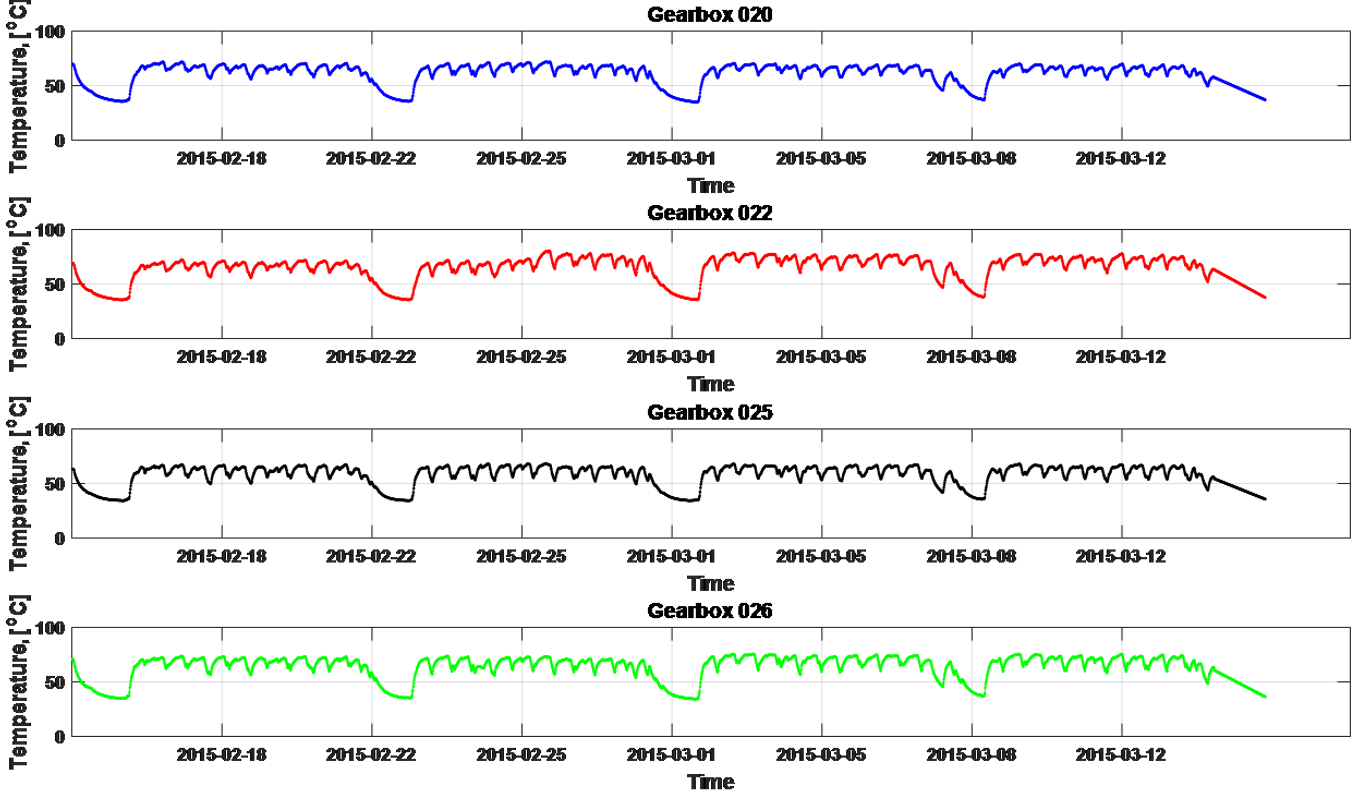
\includegraphics[width = 0.8\textwidth]{wykresy/ica_raw.png}
\caption{Preprocessed input signals.}
\label{fig: ica_raw}
\end{figure}

At first, signals had to~be preprocessed according to~methodology described in~section \ref{temp_ica}, and the~output sampling period was set to~15 minutes. First conclusion when comparing Fig \ref{fig: ica_raw} is~that looking of~each signal separately is~non-effective from diagnostic point of~view. 

% \begin{figure}[ht!]
% \centering
% 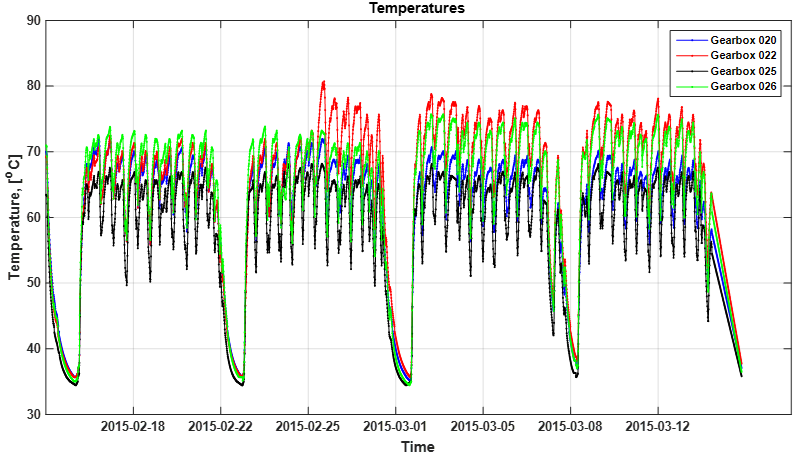
\includegraphics[width = 1\textwidth]{wykresy/ica_raw2.png}
% \caption{Signals presented together.}
% \label{fig: ica_raw2}
% \end{figure}

However, an~automatic technique is~required, that will allow to~extract process related to~change of~condition only. Hence, ICA approach was used. In this case ICA returns four features with estimated unmixing matrix $W^T$:

\begin{gather}
 W^T =
 \begin{bmatrix}
  0,469 & 0,006 & -0,504 & 0,076 \\
  -0,104 & -0,151 & -0,586 & 0,725 \\
  -0,304 & 0,335 & -0,035 & -0,019 \\
  -0,343 & -0,163 & 0,417 & 0,165
  \end{bmatrix}
\end{gather}

For reasons described in~section \ref{app_ica} arrangement of~output features will be~different every time. As we can see in~Fig. \ref{fig: ica_feat} features 1 and 4 carry information about common factors of~signals behavior, feature 2 presents highest frequency details, and feature 3 informs about trend of~behavior change, so in~this case third feature is~selected for further analysis. Besides, cross-correlation provides the~information that selected feature is~connected with behavior of~signal coming from gearbox 022.

\begin{figure}[ht!]
\centering
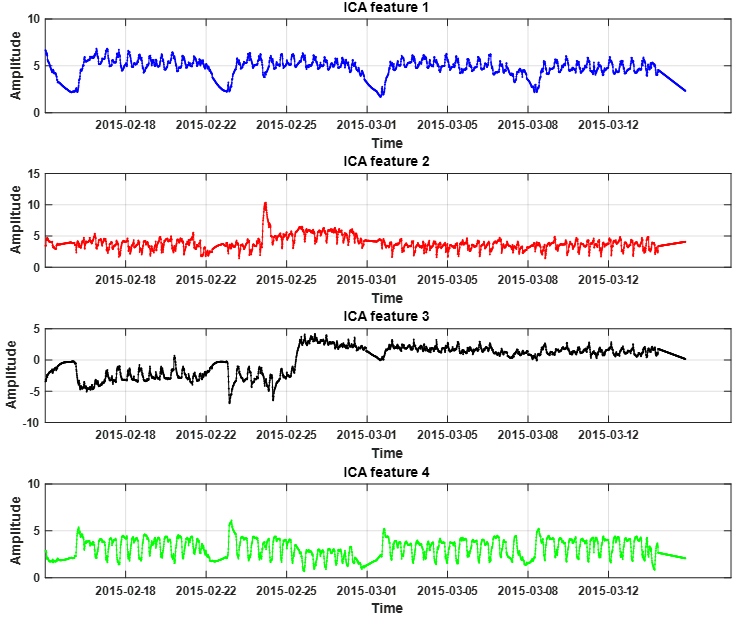
\includegraphics[width = 0.7\textwidth]{wykresy/ica_feat.png}
\caption{Four features obtained from ICA.}
\label{fig: ica_feat}
\end{figure}

Selected feature along with daily variances is~presented in~Fig. \ref{fig: ica_feat2}. One can see that two events can cause an~alarm. Event occurring during $12^{th}$ day can be~clearly visible in~the~third feature in~Fig. \ref{fig: ica_feat}. The event originates from the~signal from gearbox 022. On the~other hand, event occurring during $9^{th}$ day is~not easily visible. Fig. \ref{fig: ica_feat3} presents this situation. One can see that during $24^{th}$ of~February, temperature of~gearboxes 026 and 022 dropped unusually compared to~behavior from previous work cycles. 

\begin{figure}[ht!]
\centering
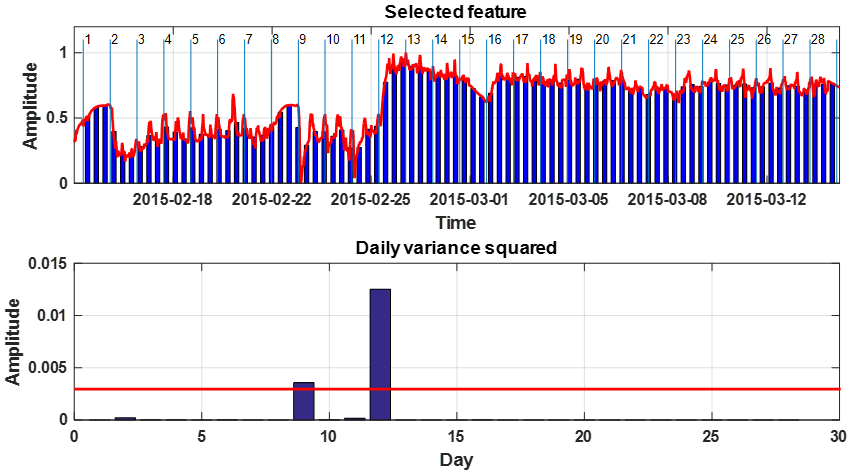
\includegraphics[width = 0.7\textwidth]{wykresy/ica_feat2.png}
\caption{Selected feature with consecutive days indicated. Daily variance squared has been proposed as~event selector.}
\label{fig: ica_feat2}
\end{figure}

\begin{figure}[ht!]
\centering
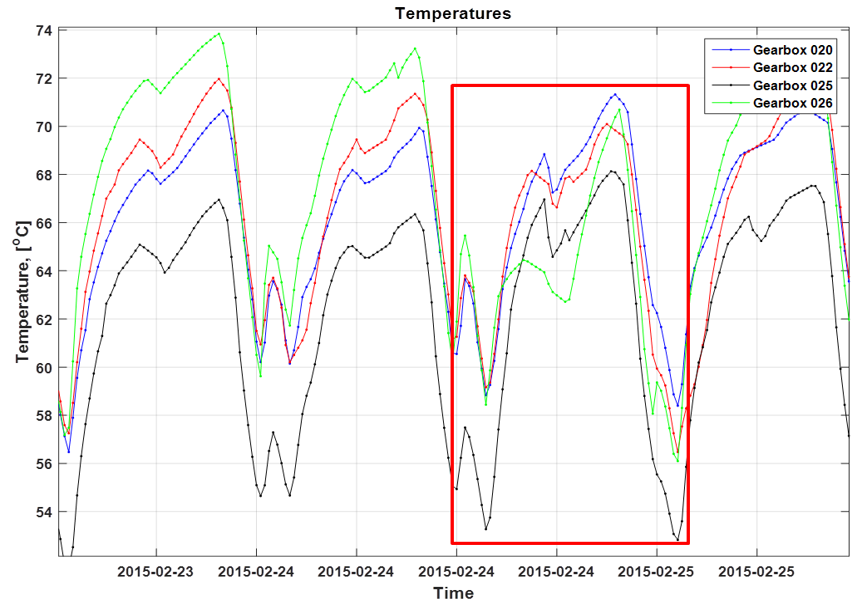
\includegraphics[width = 0.6\textwidth]{wykresy/ica_feat3.png}
\caption{Event from day 9. The unusual temperature drop on~the~gearboxes 026 and 022 also triggered the~warning indicator.}
\label{fig: ica_feat3}
\end{figure}

% \subsubsection{Summary}

% In this paper author presented application of~Independent Component Analysis for signal feature extraction applied to~real temperature signal from set of~heavy duty gearboxes used in~mining industry. The methodology is~based on~the~analysis of~multichannel time series. In order to~extract information about the~damage author analyzed the~features obtained by~applying the~ICA to~four-channel input signal. Extracted features allow to~detect unusual behavior of~gearboxes, identify misbehaving device and provide behavioral feature for further analysis and interpretation. By using ICA author was able to~separate different sources influencing shape of~measured temperature signal, or in~other words, it~is~possible to~remove contribution related to~operational factors from the~signal.

\subsection{Work regimes distinction using EM}\label{result_em}

In this section author describes how method presented in~section \ref{temp_em} was used to~analyze temperature data measured on~a~single heavy-duty gearbox used in~belt conveyor driving station in~underground mine.

Parameterization using selected statistics allowed to~construct three feature vectors presented in~the~Fig. \ref{fig: cluster_stats_day}

\begin{figure}[ht!]
\centering
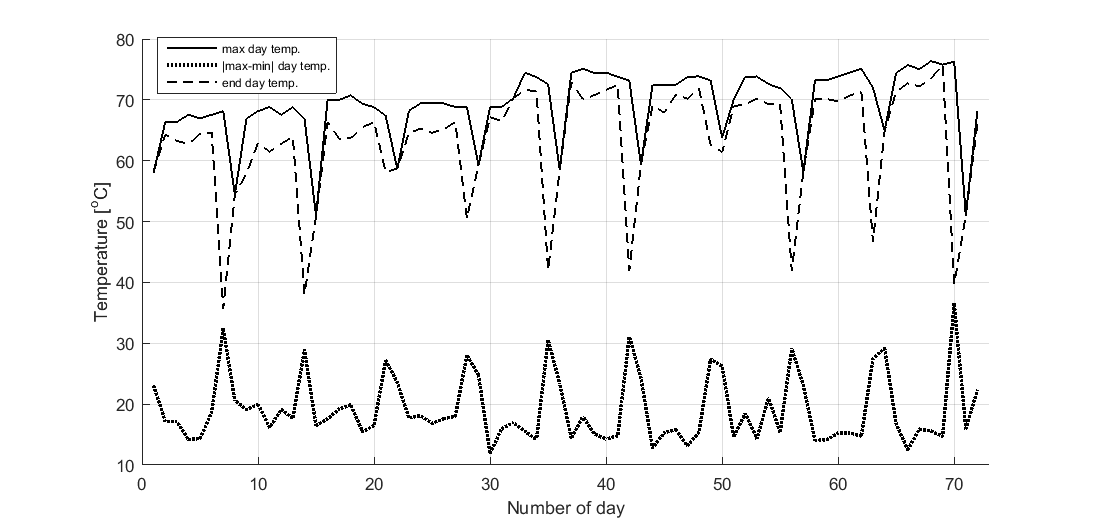
\includegraphics[width = \textwidth]{wykresy/cluster_stats_day.png}
\caption{Vectors of~statistics used in~clustering process.}
\label{fig: cluster_stats_day}
\end{figure}

Three-dimensional data points constructed from described statistic vectors distributed themselves in~the~3D feature space as~shown in~Fig \ref{fig: unclusteredbw}. It is~clearly visible that there are four or even five clusters possible to~be distinguished. For this dataset Silhouette criterion returned optimal amount of~clusters equal to~$5$ (see definition in~section \ref{app_sil}). As a~result of~presented procedure author obtained information about individual days belonging to~certain clusters (see Fig. \ref{fig: clustered}). Each cluster defines in~correct and accurate way one of~five possible outcomes:

\begin{figure}[ht!]
\centering
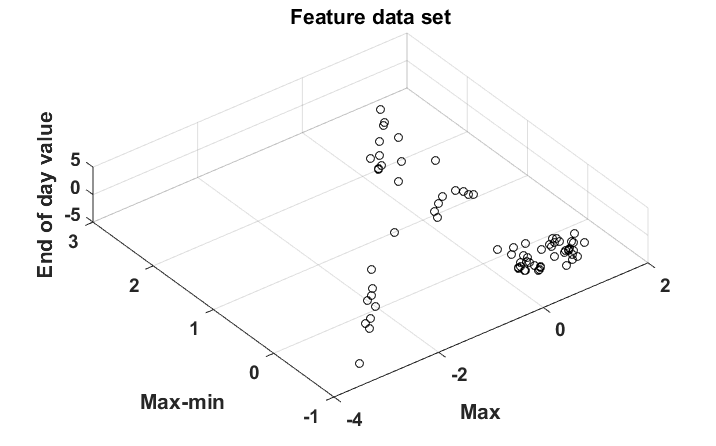
\includegraphics[width = \textwidth]{wykresy/unclusteredbw.png}
\caption{Distribution of~points in~3D feature space.}
\label{fig: unclusteredbw}
\end{figure}

\begin{itemize}
\renewcommand{\labelitemi}{$\bullet$}
\item Mondays,
\item Saturdays,
\item Sundays,
\item Other days of~the~week in~good condition,
\item Other days of~the~week in~bad condition.
\end{itemize}

All of~those classes are important to~be detected and identified. Mondays, Saturdays and Sundays reveal very outlying behavior, hence they are not informative and are detected only to~be eliminated from further analysis. On the~other hand, theoretically all days of~the~week could be~divided into classes of~good and bad conditions, but it~was impossible for such limited amount of~data. Longer data record might cause points in~feature space to~fill cavities within the~clusters. Because of~that, point clouds would be~denser and more consistent. It would allow the~Silhouette criterion to~estimate larger optimal cluster amount, which then could possibly lead to~distinction between good and bad condition on~Mondays, Saturdays and Sundays.

\begin{figure}[ht!]
\centering
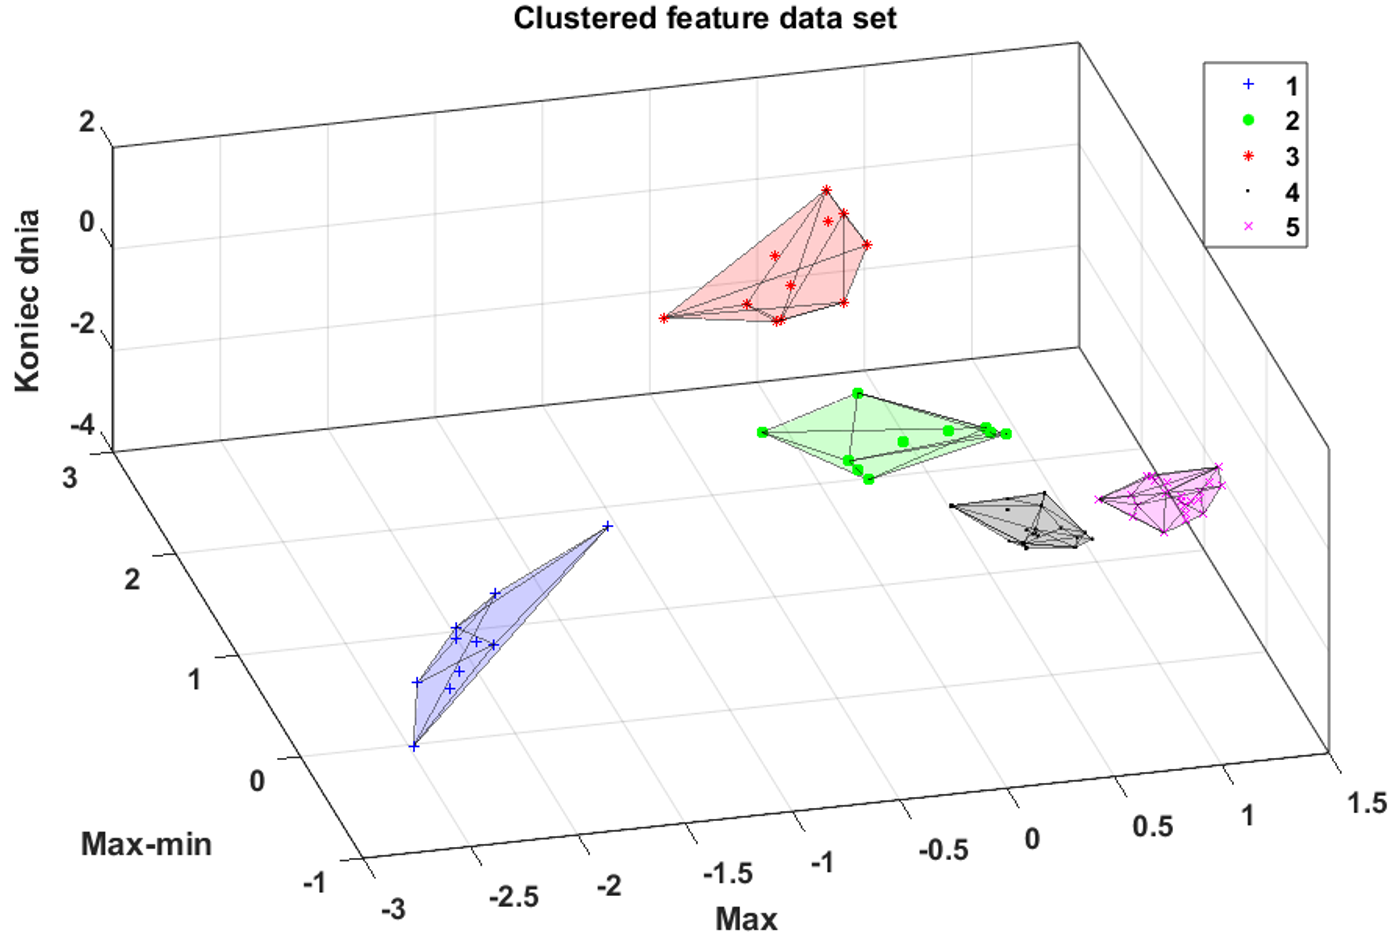
\includegraphics[width = \textwidth]{wykresy/clustered.png}
\caption{Clustering results in~feature space (values normalized). Clusters represent Sundays (1), Saturdays (2), Mondays (3), other days in~good condition (4), and other days in~bad condition (5).}
\label{fig: clustered}
\end{figure}

Fig. \ref{fig: cplot} presents the~results in~time domain. One can clearly see that EM algorithm correctly assigned particular days to~their respective classes.

\begin{figure}[ht!]
\centering
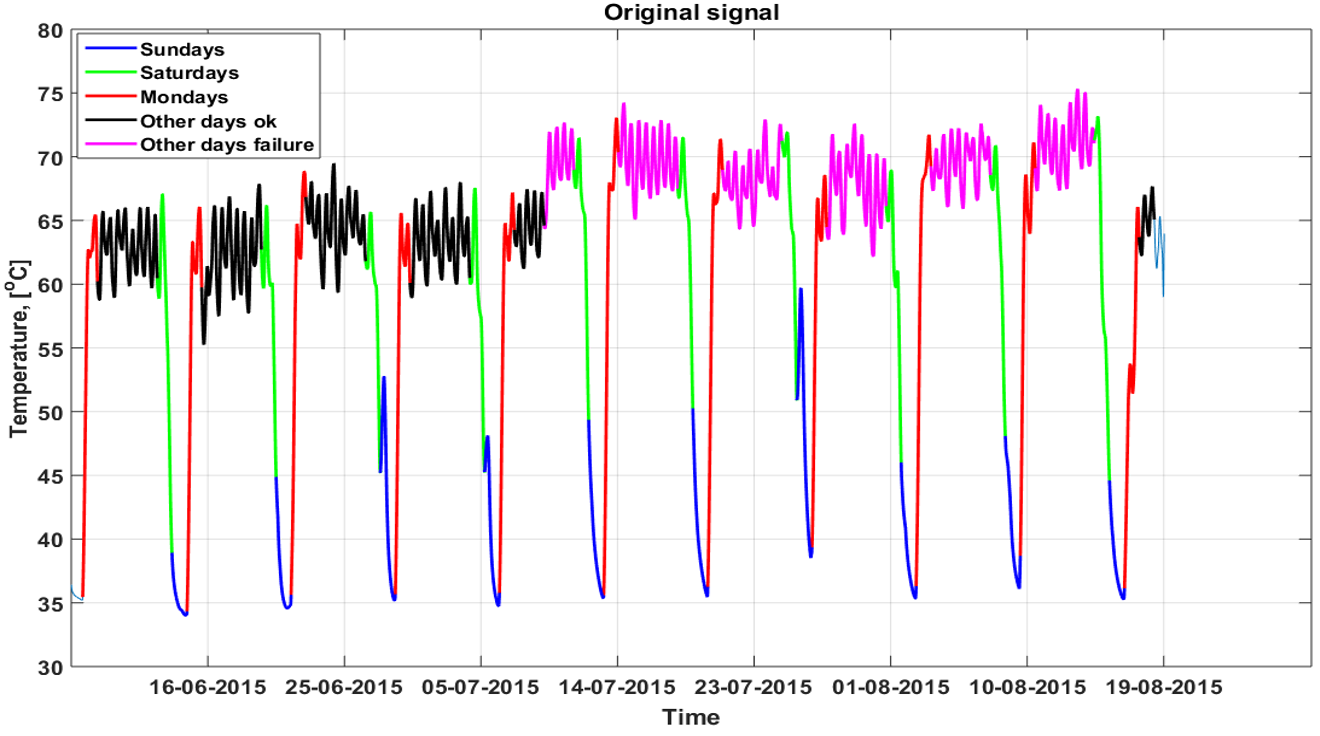
\includegraphics[width = \textwidth]{wykresy/cplot.png}
\caption{Clustering results in~time domain.}
\label{fig: cplot}
\end{figure}

\subsection{Time-time map analysis for LHD fault detection}\label{real_bulgaria}

\subsubsection{Data description}

Measured data originate from the~built-in data acquisition system provided by~the~manufacturer of~LHD machines. In this work author focused only on~one variable describing temperature of~engine coolant. Data has been provided with sampling period of~30 seconds, which is~enough in~case of~slowly varying values such as~temperature. Data describes period of~about two and a~half months (see Fig. \ref{fig: lhd_temp_raw}).

\begin{figure}[ht!]
\centering
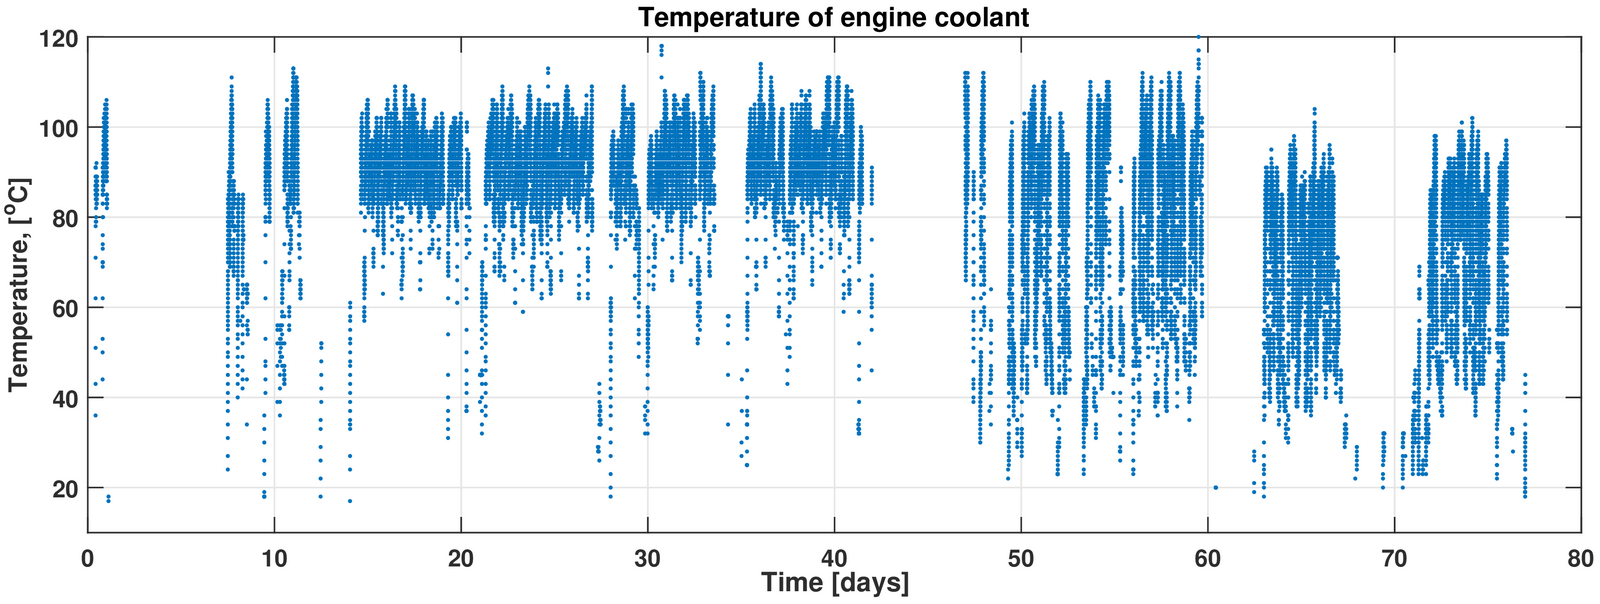
\includegraphics[width = \textwidth]{wykresy/lhd_temp_raw.png}
\caption{Raw time series of~input data.}
\label{fig: lhd_temp_raw}
\end{figure}

According to~preprocessing described in~section \ref{temp_bulgaria} data has been transformed to~time-time representation (see Fig. \ref{fig: lhd_temp_map}).

\begin{figure}[ht!]
\centering
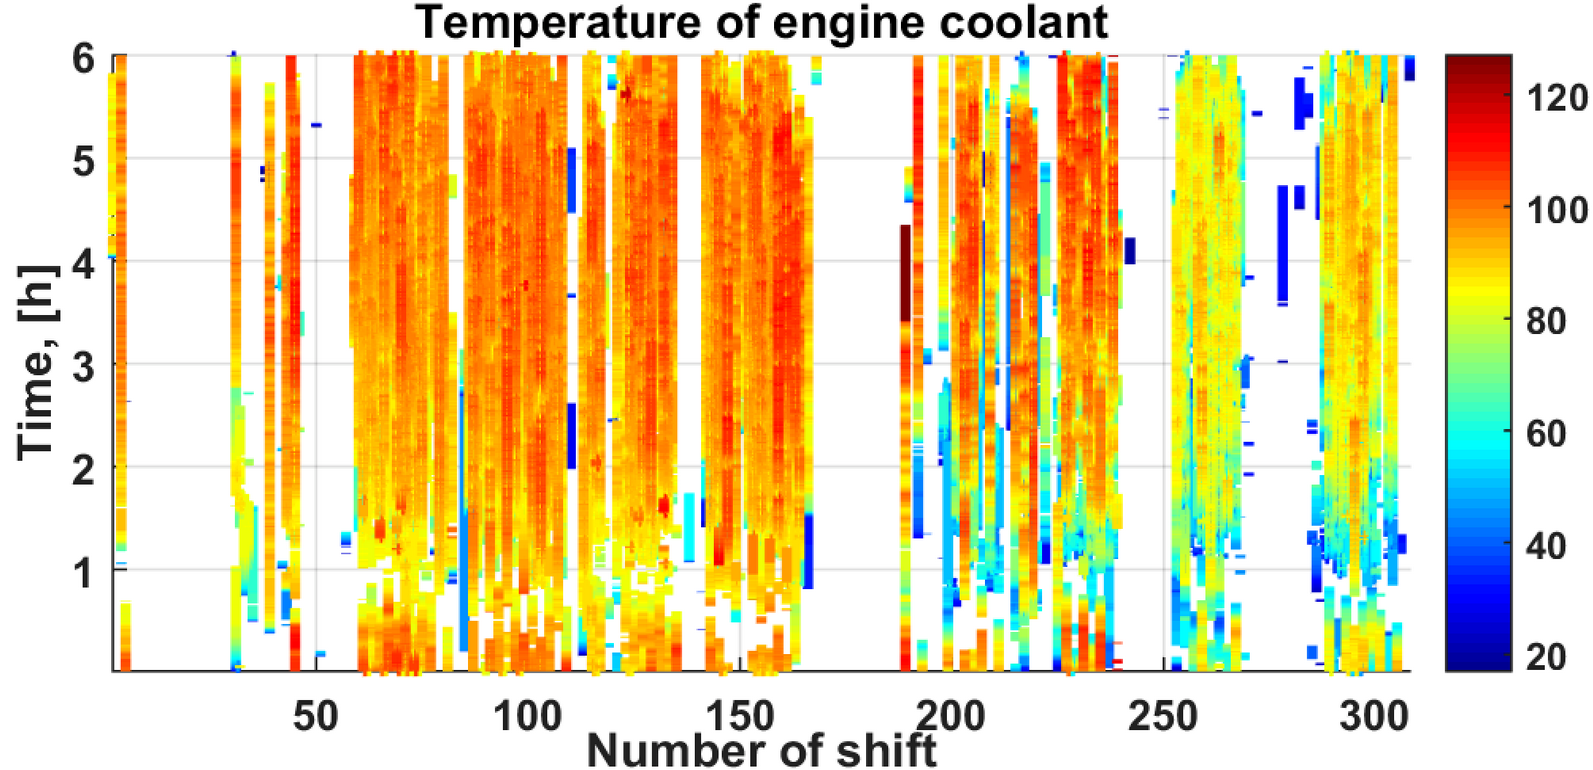
\includegraphics[width = \textwidth]{wykresy/lhd_temp_map.png}
\caption{Map of~engine coolant temperature values along consecutive shifts. Colors represent temperature values.}
\label{fig: lhd_temp_map}
\end{figure}

After disregarding empty and nearly empty work shifts (see Fig. \ref{fig: lhd_temp_map2}) the~first step was to~calculate probability density map and smooth it. Fig. \ref{fig:ks_maps} presents probability density maps: raw (left panel) and smoothed (right panel).

\begin{figure}[ht!]
\centering
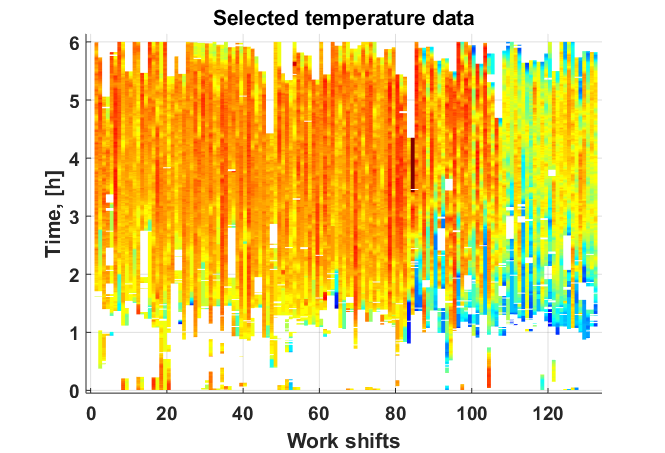
\includegraphics[width = 0.8\textwidth]{wykresy/lhd_temp_map2.png}
\caption{Remaining temperature data after selection.}
\label{fig: lhd_temp_map2}
\end{figure}

\begin{figure}[!ht]
 \centering
 \begin{subfigure}
   \centering
   % \captionsetup{skip=0.01pt}
   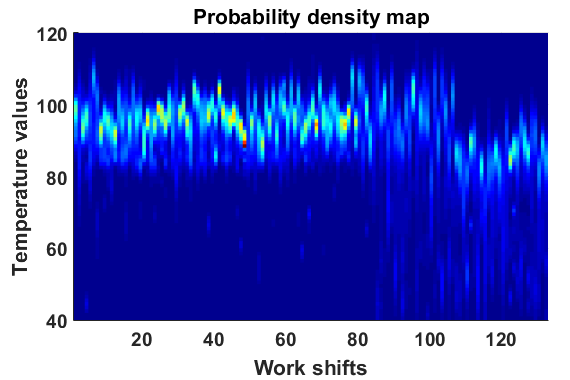
\includegraphics[width=0.49\textwidth]{wykresy/ks_map.png}
  %  \caption{Input data in~time-time domain}
   \label{fig:ks_map}
 \end{subfigure}
 %\hfill
 \begin{subfigure}
   \centering
  % \captionsetup{skip=0.01pt}
		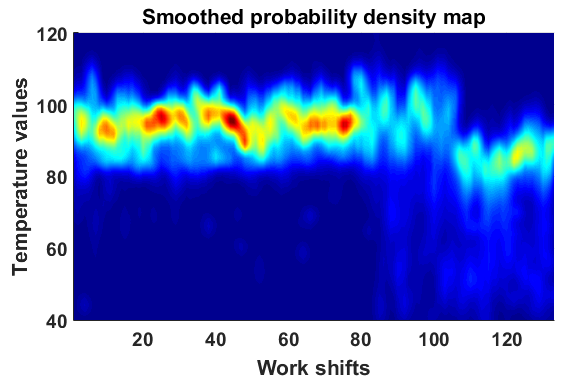
\includegraphics[width=0.49\textwidth]{wykresy/ks_map2.png}
    % \caption{Selected interpolated shifts}
  \label{fig:ks_map2}
 \end{subfigure}
 \caption{Probability density map created from raw data (left panel) and smoothed map (right panel). Smoothing the~data results in~more consistent behavior of~the~calculated statistics.}
 \label{fig:ks_maps}
\end{figure}

It can be~easily seen that data is~divided into three main health states that change at~two points: at~about $80^{th}$ shift and at~about $110^{th}$ shift counting according to~the~density map. First state is~characterized with relatively low dispersion of~data values as~well as~overall symmetry and stability of~data distributions. 

\begin{figure}[ht!]
\centering
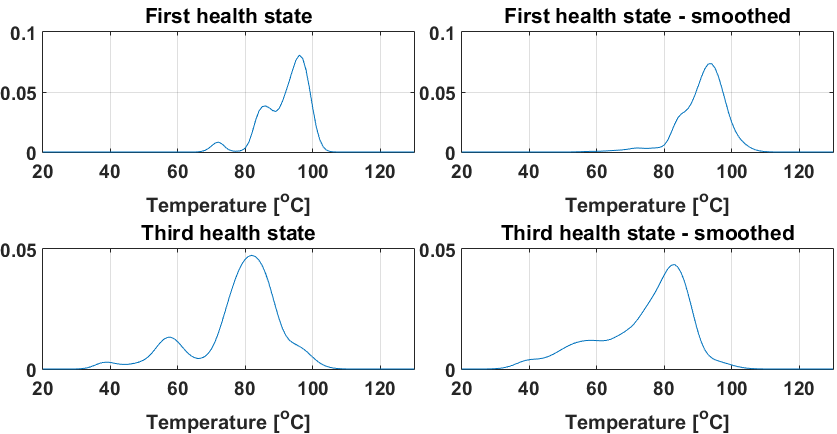
\includegraphics[width = 0.8\textwidth]{wykresy/ks_ex.png}
\caption{Examples of~density functions selected from first health state (top panels) and third health state (bottom panels) drawn from raw density map (left panels) and smoothed density map (right panels).}
\label{fig: ks_ex}
\end{figure}

The second one reveals sudden increase of~data dispersion with appearance of~negative skewness of~the~distributions with preservation of~fundamental mode position. Third state also indicates negative skewness and higher dispersion than the~first one, but fundamental mode of~the~distributions is~shifted significantly towards lower values. It is~clearly visible that difference between density functions from different health states is~significant and can allow to~identify and segment health states (see Fig. \ref{fig: ks_ex}).

\begin{figure}[ht!]
\centering
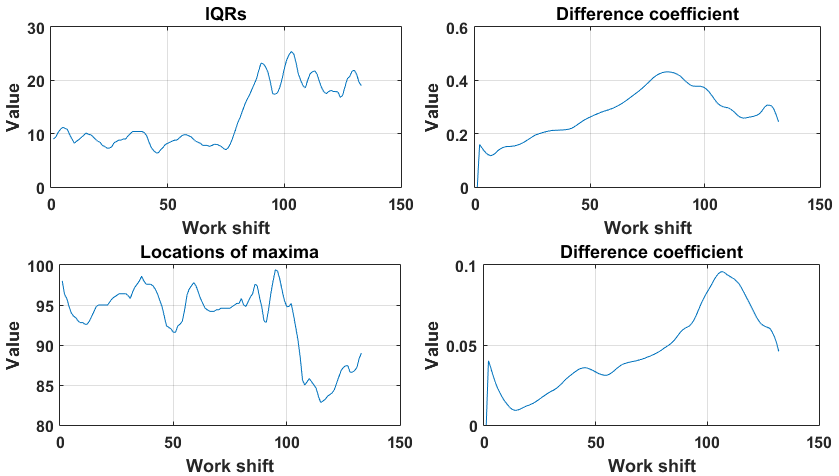
\includegraphics[width = 0.8\textwidth]{wykresy/ks_stats.png}
\caption{Operational statistics (left panels) and their difference coefficients (right panels).}
\label{fig: ks_stats}
\end{figure}

Calculated statistics and their difference coefficients are shown on~Fig. \ref{fig: ks_stats}. In practice author calculated this coefficient for every splitting point, and then found the~maximum of~such vector. It can be~seen that each statistic clearly indicates one of~regime shifts in~the~data.

\begin{figure}[ht!]
\centering
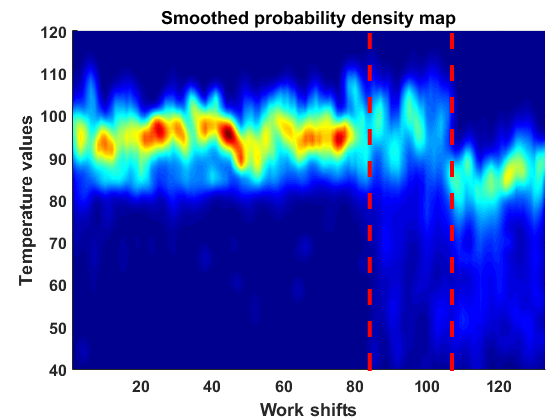
\includegraphics[width = 0.6\textwidth]{wykresy/ks_map3.png}
\caption{Localized regime shifts presented on~density map.}
\label{fig: ks_map3}
\end{figure}

Regime shifts have been localized and overlaid on~probability density map (see Fig. \ref{fig: ks_map3}) and on~original temperature time series (see Fig. \ref{fig: ks_final}). For this data sample they were identified to~be shifts no. $189$ and $253$ counting within all shifts before empty values removal, or shifts no. $84$ and $107$ counting according to~density map. 

It is~very important to~mention that accounting system of~the~mine reports the~repair performed on~the~machine on~the~day $108$, that was connected to~the~engine overheating problem. 

\begin{figure}[ht!]
\centering
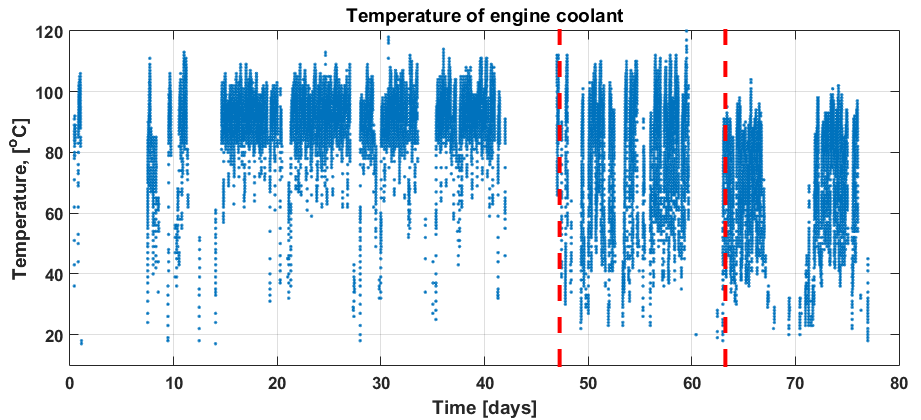
\includegraphics[width = \textwidth]{wykresy/ks_final.png}
\caption{Localized regime shifts presented on~raw data.}
\label{fig: ks_final}
\end{figure}

Considering that presented method uses data smoothing and probabilistic techniques that can in~theory decrease precision of~calculations, difference of~only one day between date of~second found regime shift and date of~reported repair is~surprisingly small, and concludes high quality of~the~method. Presented method correctly identifies changes in~characteristics of~operation, basing on~the~temperature data of~engine coolant. Tracking and interpretation of~those changes might be~used to~prepare preventive maintenance scenarios for the~machine, and prolong its lifespan in~the~long run. 

\subsection{Anderson-Darling statistic map for failure detection}\label{real_ad}

In this section presented method described in~section \ref{temp_ad} is~applied to~real-life temperature data. Method is~operating on~data already described in~section \ref{real_bulgaria}, and preprocessing stage that constructs time-time representation is~identical (see Fig. \ref{fig: lhd_temp_map2}).

\begin{figure}[!ht]
 \centering
 \begin{subfigure}
   \centering
   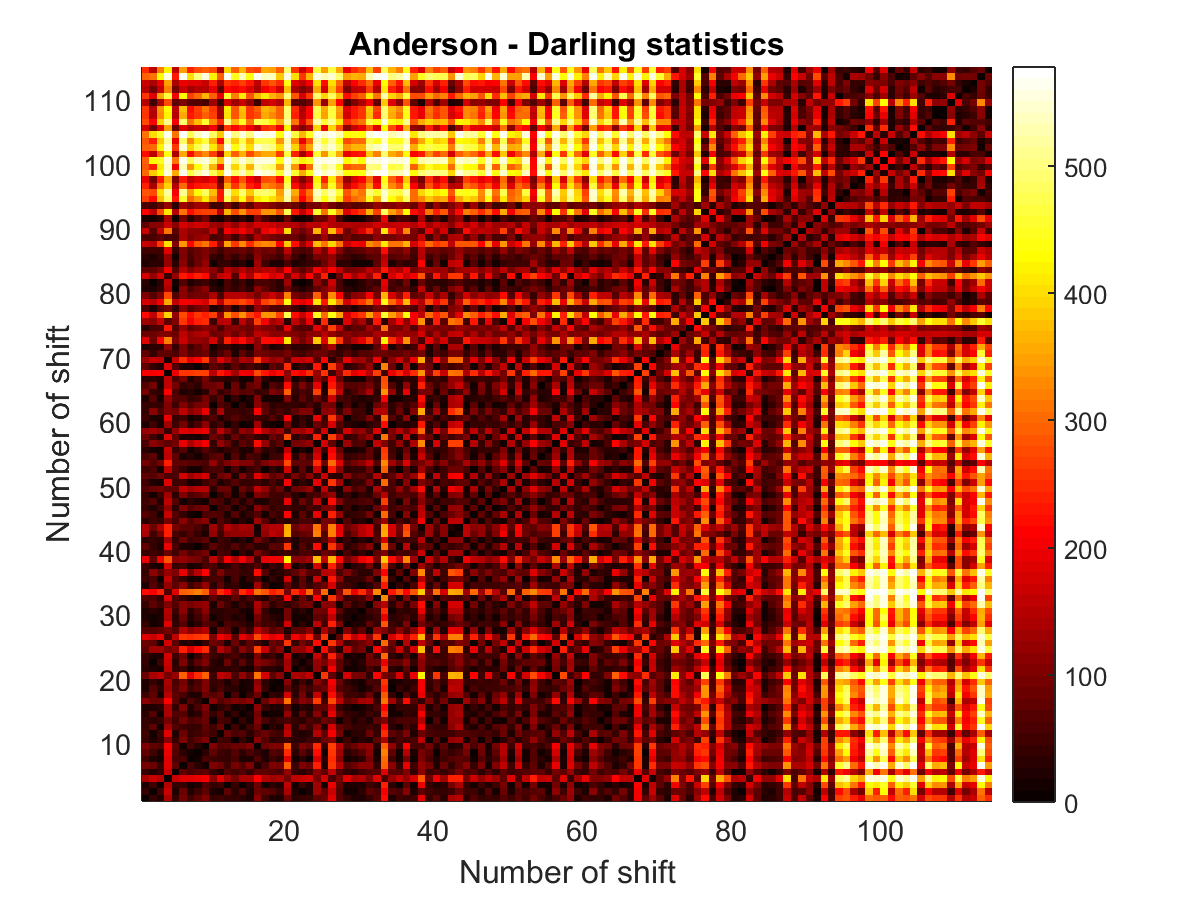
\includegraphics[width=0.48\textwidth]{wykresy/ADK-stat}
 \end{subfigure}
 \begin{subfigure}
   \centering
		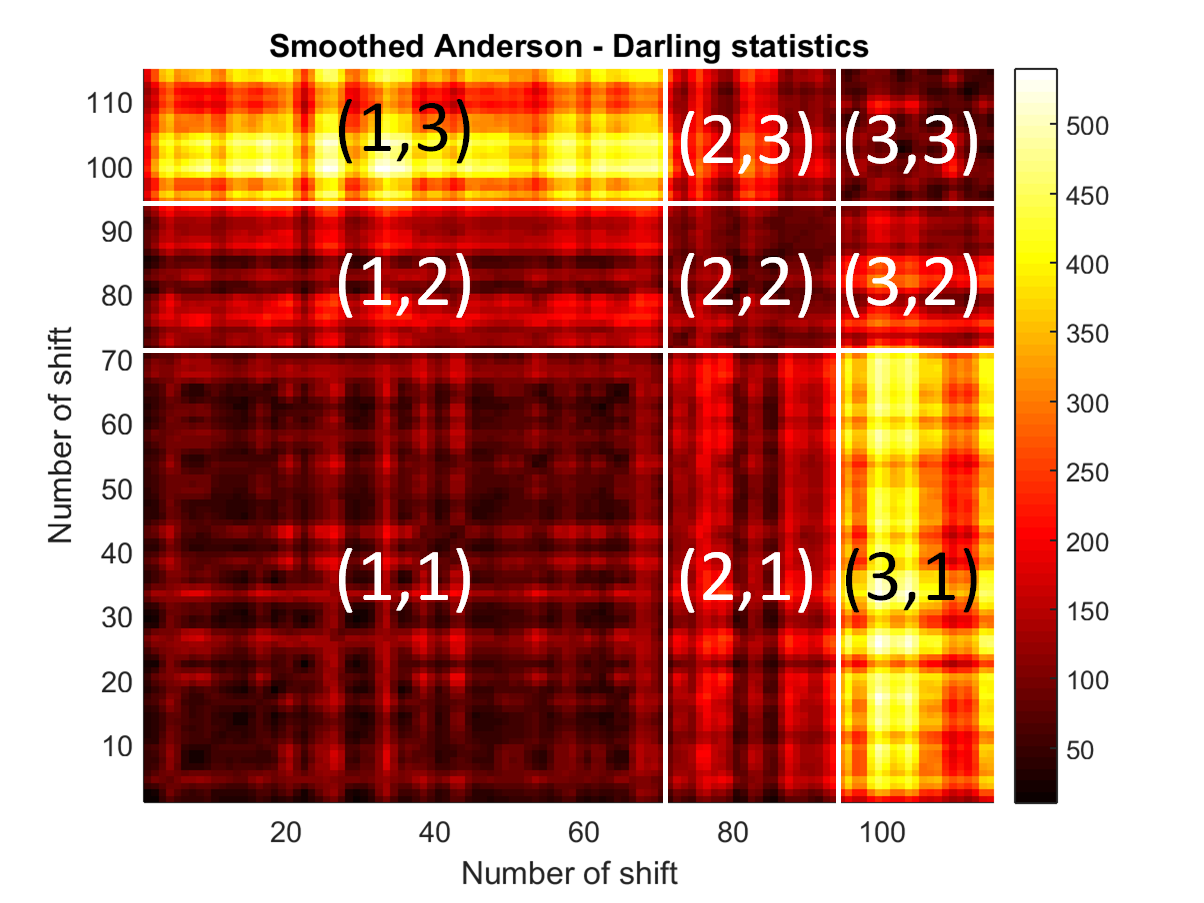
\includegraphics[width=0.48\textwidth]{wykresy/ADK-stat-smooth2}
 \end{subfigure}
 \caption{Anderson-Darling statistic map (left panel) and the~same map after filtering with triangular kernel (right panel) with notation corresponding to~Fig. \ref{fig:map}}
 \label{fig:ADK-stat-2}
\end{figure}

Left panel of~Figure \ref{fig:ADK-stat-2} shows the~values of~Anderson-Darling statistics for each pair of~compared work shifts. Areas connected to~described processes are visible, but after filtration properties of~the~map are enhanced (see Fig. \ref{fig:ADK-stat-2} right panel).

\begin{figure}[!ht]
 \centering
 \begin{subfigure}
   \centering
   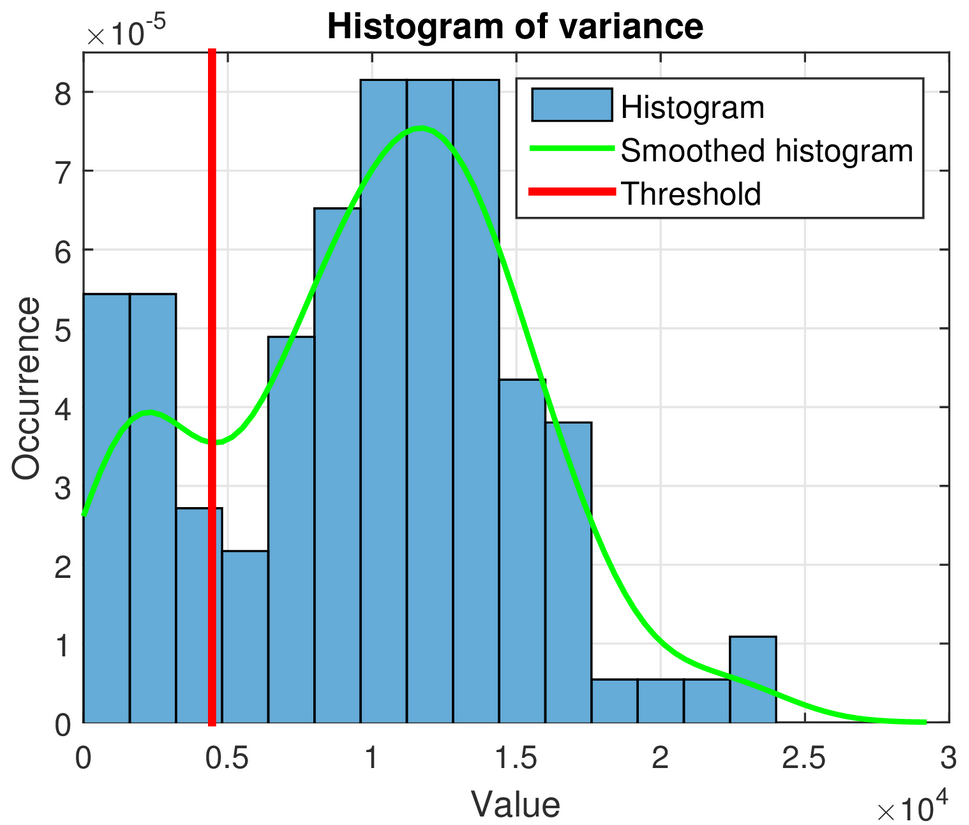
\includegraphics[width=0.48\textwidth]{wykresy/ksd}
 \end{subfigure}
 \begin{subfigure}
   \centering
		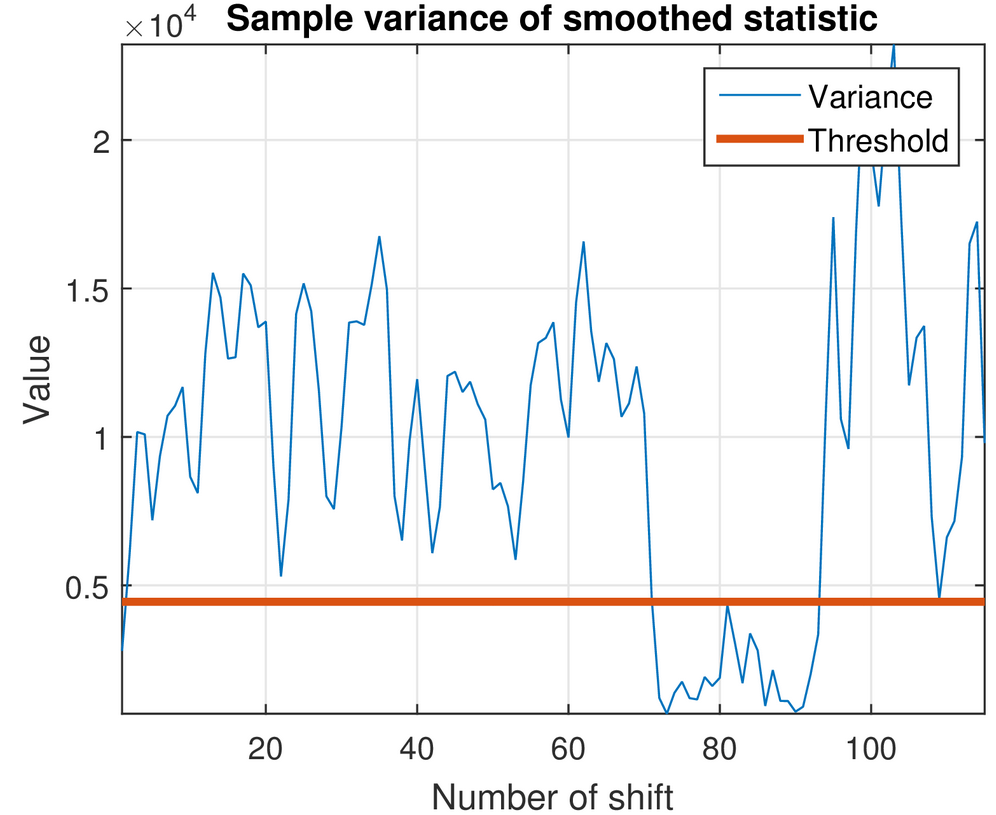
\includegraphics[width=0.48\textwidth]{wykresy/ADK-thr}
 \end{subfigure}
 \caption{One-dimensional sample variance of~filtered AD map thresholded by~local minimum of~smoothed histogram of~the~variance vector}
 \label{fig:ADK-KS-thr}
\end{figure}

After filtering AD map, sample variance of~column vectors is~calculated. The values of~variance for each work shifts are presented in~right panel of~Fig. \ref{fig:ADK-KS-thr} (blue line). Next step is~to~estimate its distribution by~smoothed histogram and calculate local minimum of~this function (see left panel of~Fig. \ref{fig:ADK-KS-thr}). Author proposes to~take this value as~a~threshold (red line in~right panel of~Fig. \ref{fig:ADK-KS-thr}). The area where variance is~smaller that threshold corresponds with failure state.

Transition points have been overlaid on~input temperature data (see Fig. \ref{fig: AD_final}). They were identified to~be at~shifts no. 166 and 238 when counting within all shifts before empty values removal, or shifts no. 72 and 93 when according to~interpolated map. It is~important to~mention that accounting system of~the~mine reports the~repair performed on~the~machine, that was connected to~the~engine overheating problem. The actual day of~repair is~the~day after detected change of~technical condition. Considering that method presented in~this paper based on~statistical analysis, smoothing and transforming from two to~one-dimensional form has only one day difference between date of~reported repair and date of~second found transition point is~surprisingly small.

\begin{figure}[ht!]
\centering
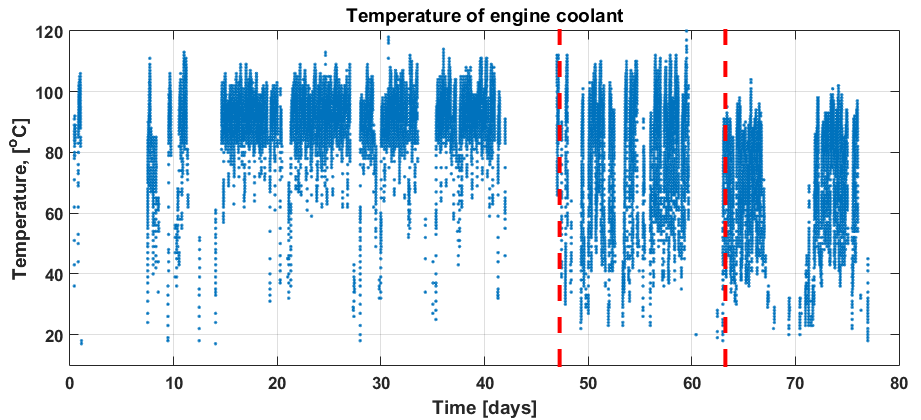
\includegraphics[width = \textwidth]{wykresy/ks_final.png}
\caption{Localized regime shifts presented on~raw data.}
\label{fig: AD_final}
\end{figure}

As a~result, long-term observation has been divided into three health states: warning state (approaching failure), state of~failure and healthy state after repair. Localized moments of~state changes have been positively verified with experts from the~mine, which confirms correctness of~obtained results and overall method performance.


\clearpage
\section{Muiltichannel spectrogram analysis using PCA}\label{result_pca}

In this section presented method described in~section \ref{met_pca} is~applied to~real-life multichannel vibration data.

\subsubsection{Data description}

The machine considered here is~a~two-stage gearbox used in~drive system for belt conveyor. Raw multichannel signal and its spectrogram representation is~shown in~Fig. \ref{fig: pca_raw} and \ref{fig: pca_spec}, respectively. Both time series and their spectrograms allow to~notice some weak impulsive/wideband components but it~is~impossible to~be distinguished unambiguously.


% The experiment shows that the~gearbox does not reveal any damage. Thus, an~artificial damage is~introduced by~specific signal processing technique in~order to~illustrate benefits of~the~proposed methodology. Namely, each of~four acquired signals is~considered as~a~response of~the~system (each signal stands for an~individual system) to~stationary noise, since there is~no damage in~the~gearbox. Thus, we fit the~autoregressive (AR) model to~each of~four signals by~Yule-Walker equations and obtain four sets of~coefficients called the~impulse responses of~the~system. Orders of~the~AR models are high enough to~reflect complexity of~amplitude spectra of~the~acquired signals. Then, four pulse trains (Kronecker combs) with additive Gaussian noise are designed as~excitation signals (source signals) that correspond to~a~damaged gearbox. Duration of~the~excitation signals is~equal to~the~duration of~signals acquired during the~experiment. The fault frequency associated to~damage in~gear-wheel on~the~middle shaft is~4.1 Hz and this is~the~frequency of~impulses in~the~pulse trains. The ratio of~impulse to~noise amplitudes is~different for each excitation signal, which corresponds to~different distance between each sensor and the~damaged gear. Finally, the~pulse trains are convolved with corresponding impulse responses and such signals are further analyzed and referred as~“raw signals”.

\begin{figure}[ht!]
\centering
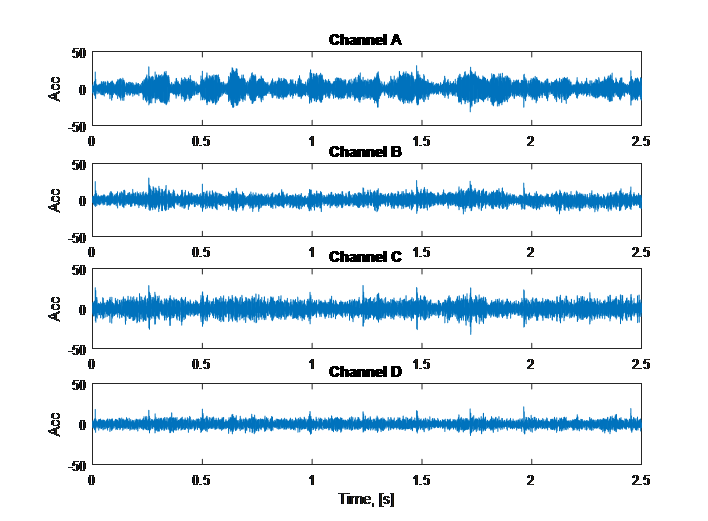
\includegraphics[width = 0.8\textwidth]{wykresy/pca_raw.png}
\caption{Multichannel input signal.}
\label{fig: pca_raw}
\vspace{-10px}
\end{figure}


\begin{figure}[ht!]
\centering
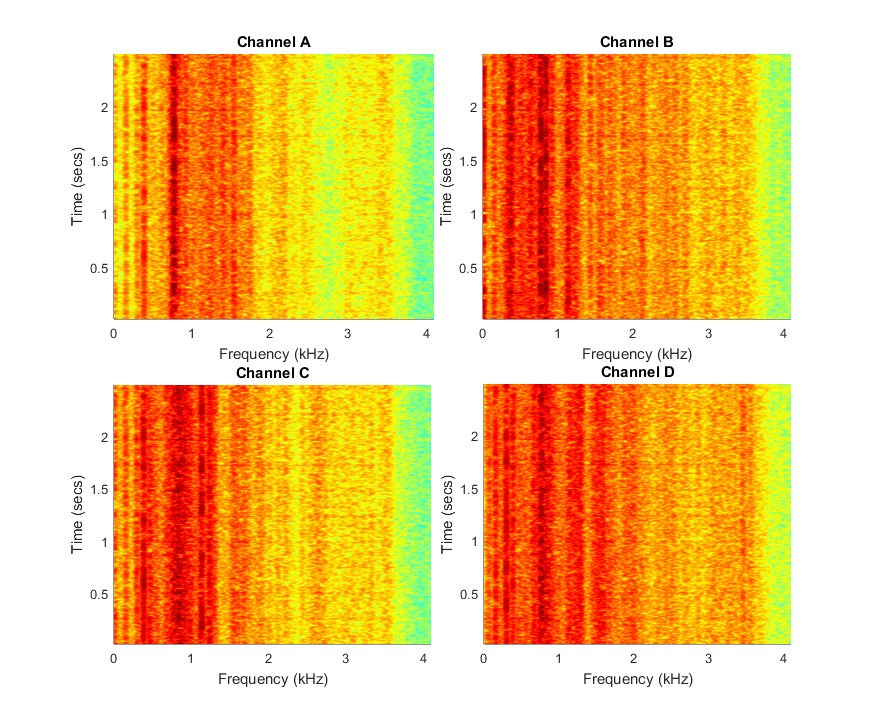
\includegraphics[width = 0.8\textwidth]{wykresy/pca_spec.png}
\caption{Spectrograms of~input signal.}
\label{fig: pca_spec}
\end{figure}

\subsubsection{Results}

In this section author presents the~results of~introduced method, i.e. performance of~the~algorithm fed with discussed data. Fig. \ref{fig: pca_out} (left panel) presents new time-frequency map which consists of~the~components extracted by~applying PCA to~the~sub-signals from the~initial spectrograms. The impulses (wideband excitations) are visible much more clearly than in~the~spectrograms of~multichannel raw signal (see Fig. \ref{fig: pca_spec}). Moreover, simple aggregation of~2D map into 1D vector by~integration of~energy for each time instance shows impulsive nature of~energy flow. Using simple spectrum one can identify period/frequency of~impulse repetition that corresponds to~fault frequency, see Fig. \ref{fig: pca_out} (right panel).

It is~also important to~note that scores of~principal components of~slices from initial spectrograms vary in~frequency domain. Although always first component was taken, its score ranged from over 0.99 for heavily impulsive frequency bins, down to~less than 0.6 for bins that did not carry as~much impulsive information.

\begin{figure}[!ht]
 \centering
 \begin{subfigure}
   \centering
   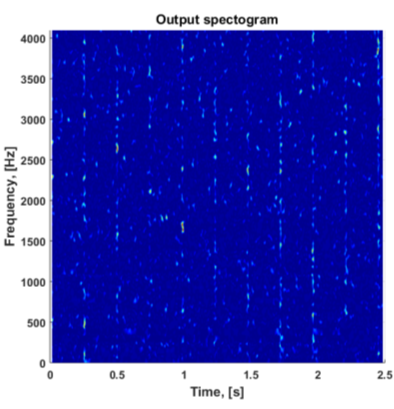
\includegraphics[width=0.48\textwidth]{wykresy/pca_outspec.png}
 \end{subfigure}
 \begin{subfigure}
   \centering
		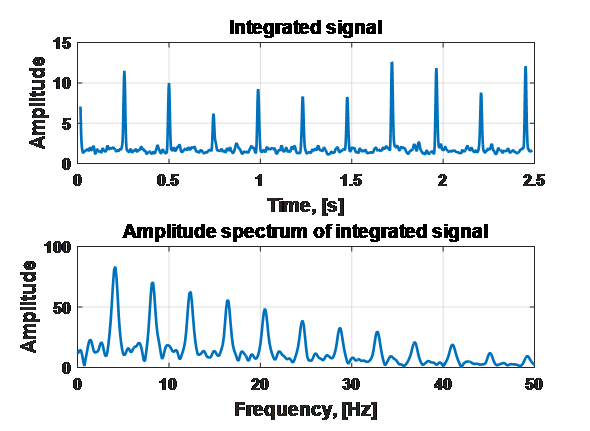
\includegraphics[width=0.48\textwidth,height=0.48\textwidth]{wykresy/pca_outts.png}
 \end{subfigure}
 \caption{Output spectrogram composed of~first PCA components (left panel). Right panels: Time series extracted from output spectrogram and spectrum of~integrated time series.}
 \label{fig: pca_out}
\end{figure}


\clearpage
\section{Methods for multidimensional domain analysis using NMF algorithms}

\subsection{STFT analysis taking advantage of~NMF encoding matrix}\label{result_enc}

In this section, author focuses on~the~analysis of~vibration data captured on~rolling bearing of~the~drive pulley according to~the~methodology described in~section \ref{met_nmf_enc}. In Fig. \ref{fig: nmf_raw} time series of~signal recorded on~the~faulty pulley bearing is~presented, and Fig. \ref{fig: nmf_spec} shows the~spectrogram of~the~signal. This data has been already analyzed in~recent papers, where several methods for local damage diagnostics have been proposed, see review in~[18]. The sampling frequency is~equal to~19.2 kHz and the~measurement is~2.5 seconds long. The spectrogram is~obtained for the~Hamming 512-sample length window with 450 overlapping samples and 512 FFT points. 

% One can notice several wide-band excitations on~the~spectrogram at~carrier frequency band 1-6 kHz that occur with the~modulation frequency of~12.7 Hz (and its multiples). This stands for outer race local damage.

\begin{figure}[ht!]
\centering
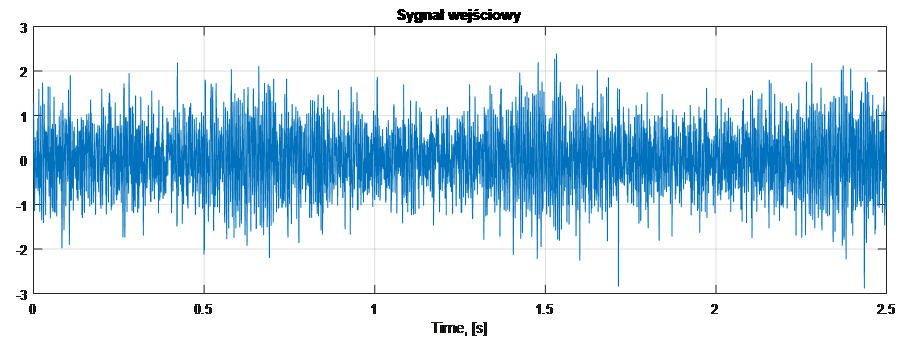
\includegraphics[width = 0.8\textwidth]{wykresy/nmf_raw.png}
\caption{Raw input signal.}
\label{fig: nmf_raw}
\end{figure}

\begin{figure}[ht!]
\centering
\includegraphics[width = 0.7\textwidth]{wykresy/nmf_spec.png}
\caption{Spectrogram of~input signal.}
\label{fig: nmf_spec}
\end{figure}

As a~next step, Semi-binary NMF algorithm groups the~spectra into three clusters (see Fig. \ref{fig: nmf_partial}) which are then transformed back to~time-series form using bulit-in Matlab procedure \texttt{istft} for Short-Time Fourier Transform inversion. Third cluster is~selected for further analysis based visual inspection (manually) or based on~maximum kurtosis of~obtained signals (automatically). The selected signal has zero value everywhere except for places where impulses occur (see Fig. \ref{fig: nmf_out} a). In those places ISTFT produced portion of~the~signal that comes from the~spectrogram slices assigned to~a~particular place (typically 3-8 slices per impulse), and hence they carry information from the~original signal (slightly suppressed by~ISTFT windowing, see Fig. \ref{fig: nmf_imp} a).

\begin{figure}[ht!]
\centering
\includegraphics[width = \textwidth]{wykresy/nmf_partial.png}
\caption{Partial spectrograms constructed based on~clustering results. Third spectrogram is~selected for further analysis.}
\label{fig: nmf_partial}
\end{figure}

The methodology is~based on~nonnegative matrix factorization of~the~spectrogram, but it~should be~mentioned that the~algorithm can be~applied to~other multidimensional representations of~the~input signal. 

\begin{figure}[ht!]
\centering
\includegraphics[width = 0.8\textwidth]{wykresy/nmf_out.png}
\caption{Recovered time series: a) after ISTFT transformation from selected partial spectrogram, b) after further highpass filtration.}
\label{fig: nmf_out}
\end{figure}

To extract proper shape of~the~impulse we perform filtration of~obtained signal with finite impulse response (FIR) highpass filter using the~Kaiser window with the~cutoff frequency equal to~1300 Hz (obtained as~optimal for maximizing SNR value), the~stopband attenuation of~-15 dB (parameters optimized for the~highest SNR). It removes low-frequency high-energy components from the~signal, and retains the~information about the~actual impulse (see Fig. \ref{fig: nmf_imp} b).

\begin{figure}[ht!]
\centering
\includegraphics[width = 0.7\textwidth]{wykresy/nmf_imp.png}
\caption{Example of~impulse shape before and after filtration.}
\label{fig: nmf_imp}
\end{figure}

Obtained filtered signal contains detected impulses caused by~local damage of~the~bearing (see Fig. \ref{fig: nmf_out} b). Further analysis of~signal structure (e.g. spectral analysis) and correlating the~results with the~knowledge about the~machine kinematics can provide information leading to~identification of~precise origin of~the~damage.

\subsection{STFT analysis taking advantage of~NMF base matrix}\label{result_base}

In this section author presents the~application of~extraction method proposed in~section \ref{met_nmf_base} to~the~real-life vibration signal from copper ore crusher operating in~mining industry. 


% Since there was no available signal from faulty crusher (all machines turned out to~be in~good technical condition), an~artificial damage has been introduced to~healthy signal to~simulate cyclic damage. Component has been introduced in~a~way that it~is~not directly visible in~the~time series (Fig. \ref{fig: nmfb_raw}) or in~the~envelope spectrum (Fig. \ref{fig: nmfb_widma} top).

\begin{figure}[!ht]
\centering
\includegraphics[width = 0.7\textwidth]{wykresy/nmfb_raw}
\caption{Input vibration signal of~the~ore crusher}
\label{fig: nmfb_raw}
\end{figure}

In Fig. \ref{fig: nmfb_raw} input vibration signal is~presented. Time series reveals numerous high-energy wideband impulses being the~result of~rocks falling into the~machine. On the~other hand, cyclic damage component is~barely noticeable above the~noise floor. Parameters of~spectrogram calculated for this dataset are presented in~Table \ref{tab:tab2}.Time-frequency representation of~data is~presented in~Fig. \ref{fig: nmfb_spec}.


\begin{table}[ht!]
  \centering
  \caption{Parameters of~spectrogram}
 \begin{tabular}{|l|l|}
  \hline
  \textbf{Parameter} & \textbf{Value} \\ \hline
     Signal length & 10 second (240000 samples) \\ \hline
     Sampling frequency & 24000 Hz \\ \hline
     Window & Hamming, 256 samples \\ \hline
     Overlap & 215 samples \\ \hline
     FFT points & 512 samples \\ \hline
     Spectrogram size & $257 \times 6404$ \\

  \hline
  \end{tabular}
  \label{tab:tab2}
\end{table}

One can notice heavy impulses across almost entire frequency dimension, while the~cyclic component is~weak and located in~the~frequency band roughly between 2200 Hz and 4800 Hz. Hence real signal is~more complicated in~its structure than the~simulated one, the~optimal amount of~clusters had to~be evaluated.

\begin{figure}[!ht]
\centering
\includegraphics[width = 0.6\textwidth]{wykresy/nmfb_spec}
\caption{Time-frequency representation of~the~input signal from the~ore crusher}
\label{fig: nmfb_spec}
\end{figure}

According to~Silhouette criterion (see section \ref{app_sil}) \cite{kaufman2009finding,rousseeuw1987silhouettes}, the~optimal number of~groups is~6. The real signal is~complex and contains more different components, therefore it~is~reasonable to~use more clusters than in~simulated data.

\begin{figure}[!ht]
\centering
\includegraphics[width = 0.7\textwidth]{wykresy/nmfb_profiles}
\caption{Matrix W containing IFB selectors obtained by~NMF for the~ore crusher}
\label{fig: nmfb_profiles}
\end{figure}

In the~next step spectrogram matrix of~the~signal has been provided to~the~NMF algorithm for selector extraction (see Fig. \ref{fig: nmfb_profiles}). From the~point of~view of~presented research two selectors are especially interesting: the~one for non-cyclic impulses describing rock impacts, and the~one for cyclic impulsive component describing the~damage. Regarding obtained results, they are the~classes no. 2 and 3 respectively. Fig. \ref{fig: nmfb_filt} shows the~same data in~the~form of~plots.

\begin{figure}[!ht]
\centering
\includegraphics[width = 0.7\textwidth]{wykresy/nmfb_filt}
\caption{Plot of~IFB selectors for detected components for the~ore crusher}
\label{fig: nmfb_filt}
\end{figure}

Selection of~classes has been done using kurtosis. After its evaluation for each cluster, 2 components with greatest values (produced by~filters 2 and 3) are selected for final evaluation. Fig. \ref{fig: nmfb_out} shows the~results of~filtration.

% \begin{figure}[!ht]
% \centering
% \includegraphics[width = 0.6\textwidth]{wykresy/nmfb_out}
% \caption{Results of~filtration for the~ore crusher. Top: original signal, middle: non-cyclic component, bottom: cyclic component}
% \label{fig: nmfb_out}
% \end{figure}

\begin{figure}[!ht]
 \centering
 \begin{subfigure}
   \centering
   \includegraphics[width=0.48\textwidth]{wykresy/nmfb_out}
 \end{subfigure}
 \begin{subfigure}
   \centering
		\includegraphics[width=0.45\textwidth]{wykresy/nmfb_widma}
 \end{subfigure}
 \caption{Results of~filtration for the~ore crusher. Top: original signal, middle: non-cyclic component, bottom: cyclic component}
 \label{fig: nmfb_out}
\end{figure}

As one can see, in~case of~input signal the~damage is~not visible either in~the~time series, or in~the~envelope spectrum (Fig. \ref{fig: nmfb_out} top). It is~very clear that overwhelming fraction of~the~signal information content is~occupied by~non-cyclic impulses as~well as~background components, since time series as~well as~envelope spectrum look almost exactly the~same for input signal and for extracted non-cyclic component (see Fig. \ref{fig: nmfb_out} middle).

On the~other hand, initially invisible damage component is~successfully extracted (Fig. \ref{fig: nmfb_out} bottom) and its envelope spectrum reveals clear information about the~fundamental and harmonic frequencies of~the~damage. IFB determined for this component spans the~frequencies between 3370 Hz and 4736 Hz of~the~carrier (see Fig. \ref{fig: nmfb_filt}).

% \begin{figure}[!ht]
% \centering
% \includegraphics[width = 0.5\textwidth]{wykresy/nmfb_widma.png}
% \caption{Envelope spectra of~the~results for the~ore crusher: a) original signal, b) non-cyclic component, c) cyclic component}
% \label{fig: nmfb_widma}
% \end{figure}

\subsection{CSC analysis taking advantage of~complete NMF output}\label{result_both}

In this section author presents the~application of~extraction method proposed in~section \ref{met_nmf_both} to~the~real-life vibration signal from reciprocating gas compressor operating in~oil extraction industry.

\subsubsection{Stage 1: Preconditioning}

Figure \ref{fig:csc_raw_spec} presents the~spectrogram of~input data shown in~Figure \ref{fig:csc_raw}. While shaft-related cyclic behavior is~noticeable, SOI-related periodicity is~not detectable based on~such representation. The same result can be~observed in~the~envelope spectrum of~the~signal (see Fig. \ref{fig:csc_raw_env}), which is~the~reason of~employing different domain.

\begin{figure}[ht!]
\centering
\includegraphics[width=0.8\textwidth]{wykresy/csc_raw}
\caption{Raw vibration data}
\label{fig:csc_raw}
\end{figure}

\begin{figure}[ht!]
\centering
\includegraphics[width=0.8\textwidth]{wykresy/csc_raw_spec.png}
\caption{Spectrogram of~the~input vibration data}
\label{fig:csc_raw_spec}
\end{figure} 

\begin{figure}[ht!]
\centering
\includegraphics[width=0.8\textwidth]{wykresy/csc_raw_env.png}
\caption{Envelope spectrum of~the~input vibration data}
\label{fig:csc_raw_env}
\end{figure}

Firstly, CSC map is~calculated (see Fig. \ref{fig:csc}) from the~input signal. After primary factorization with NMF algorithm set to~2 classes, author takes advantage of~base matrix that contains set of~filters calculated for this particular CSC map. Figure \ref{fig:csc_trans} presents it~on~bottom left panel as~a~two-row matrix with carrier frequency axis common for filter bank and CSC map. On the~right panels filters are drawn conventionally. 

\begin{figure}[ht!]
\centering
\includegraphics[width=0.8\textwidth]{wykresy/csc}
\caption{Cyclic Spectral Coherence map for the~first stage}
\label{fig:csc}
\end{figure}



\begin{figure}[ht!]
\centering
\includegraphics[width=0.8\textwidth]{wykresy/csc_trans}
\caption{Construction of~filter bank using NMF base matrix}
\label{fig:csc_trans}
\end{figure}

After that input signal is~filtered with every filter from the~bank (Figure \ref{fig:csc_out} left panels) and envelope spectra of~obtained output signals are calculated for the~evaluation of~spectral structure (Figure \ref{fig:csc_out} right panels). Envelope spectrum of~the~second cluster contains fundamental frequency component of~$12,35$ Hz and its harmonics that are the~indicators of~the~rotational speed of~the~compressor shaft. On the~other hand, the~first cluster reveals the~fundamental frequency of~$127,9$ Hz and its harmonics, that additionally occur with very regular sidebands. Fundamental frequency perfectly corresponds with the~expected frequency of~BPFI for this bearing, while the~presence of~sidebands suggests the~cyclic modulation in~the~signal that is~also very common in~cases of~local damage in~rotating elements. It is~easy to~conclude that this is~the~cluster of~interest, but this information can be~also obtained in~an~automatic way by~finding a~cluster with greatest SNR of~the~time series. Note that the~change of~scale in~the~time series for obtained clusters (scaling of~vertical axis) occurs due to~characteristic of~the~filter, that even in~the~passband takes the~values less then one, however it~does not affect the~structure of~the~signal but only its amplitude.

\begin{figure}[ht!]
\centering
\includegraphics[width=0.7\textwidth]{wykresy/csc_out}
\caption{Results of~method operation. Left panels: extracted time series, right panels: corresponding envelope spectra.}
\label{fig:csc_out}
\end{figure}

\subsubsection{Stage 2: Enhancement}

While for experienced user it~could be~possible to~identify the~character of~the~damage already, envelope spectrum is~still not very clean and a~lot of~different frequency components are present, especially within lower frequency bands and in~terms of~significant background noise. Hence, the~second stage of~presented methodology is~expected to~clean the~signal by~spatial denoising of~CSC map.

\begin{figure}[ht!]
\centering
\includegraphics[width=0.6\textwidth]{wykresy/csc_raw2}
\caption{Input signal for the~second stage}
\label{fig:csc_raw2}
\end{figure}

Input signal for this stage (being the~time series of~first cluster from first stage of~analysis, see Figure~\ref{fig:csc_raw2}) is~decomposed into CSC map of~its own (see Figure~\ref{fig:csc_csc2}). After that spatial noise model matrix is~constructed according to~description in~section~\ref{denoise} (see Figure~\ref{fig:csc_spd}) and subtracted from CSC map. This way it~is~possible to~present and utilize new denoised CSC map, that is~provided for the~third stage of~analysis (see Figure~\ref{fig:csc_csc3}).

\begin{figure}[ht!]
\centering
\includegraphics[width=0.8\textwidth]{wykresy/csc_csc2}
\caption{Cyclic Spectral Coherence map for the~second stage}
\label{fig:csc_csc2}
\end{figure}

\begin{figure}[ht!]
\centering
\includegraphics[width=0.7\textwidth]{wykresy/csc_spd}
\caption{Spatial denoising model}
\label{fig:csc_spd}
\end{figure}

\begin{figure}[ht!]
\centering
\includegraphics[width=0.7\textwidth]{wykresy/csc_csc3}
\caption{Spatially denoised Cyclic Spectral Coherence map}
\label{fig:csc_csc3}
\end{figure}

\subsubsection{Stage 3: Extraction}

At this point third stage of~analysis begins, majority of~which is~focused on~Monte Carlo iterations described in~detail in~section \ref{mcmc}. For the~purpose of~robustness NMF factorization in~this stage was set to~six classes. Figure \ref{fig:csc_enc} presents the~example of~how classes might look like in~a~single MC iteration as~an~encoding matrix, and Figure \ref{fig:csc_classes} presents them as~individual plots. It is~directly the~encoding matrix of~NMF, but its vectors are presented on~individual plots. It is~visible that top-center ($2^{nd}$) cluster contains spectrum related to~shaft rotation and bottom-left ($4^{th}$) cluster stands for the~damaged bearing signature. However, it~is~clear that in~this example spectra are not selected perfectly, which is~very common effect, easiest observable on~the~damage cluster. Desired cluster describing damage spectrum is~automatically selected with maximum value of~kurtosis of~spectrum vector. 

\begin{figure}[ht!]
\centering
\includegraphics[width=0.8\textwidth]{wykresy/csc_enc2}
\caption{Example of~encoding matrix produced by~NMF in~a~single Monte Carlo iteration}
\label{fig:csc_enc}
\end{figure}

\begin{figure}[ht!]
\centering
\includegraphics[width=0.8\textwidth]{wykresy/csc_clusters}
\caption{Example classes produced by~NMF in~a~single Monte Carlo iteration, numbers in~panel titles indicate cluster kurtosis}
\label{fig:csc_classes}
\end{figure}

Figure \ref{fig:csc_multi} presents examples of~damage cluster properly selected in~consecutive MC iterations. As explained before, those clusters will not be~identical, but most of~the~time they are mostly correct, which is~why MC technique is~used to~mitigate this effect. Finally median of~selected clusters is~calculated to~extract common components. Envelope spectrum obtained that way is~a~perfect representation of~frequency components related to~damage (see Figure \ref{fig:csc_out2}).

\begin{figure}[ht!]
\centering
\includegraphics[width=0.7\textwidth]{wykresy/csc_multi}
\caption{Examples of~selected clusters}
\label{fig:csc_multi}
\end{figure}

Note that the~amplitudes of~components are much higher in~comparison to~the~envelope spectra presented in~earlier stages of~the~method. This effect occurs because of~the~fact that presented final envelope spectrum is~in~fact obtained by~the~sum of~correlation coefficients across the~CSC map. Hence, those summation can produce such high values. As it~was stated before, the~goal is~to~obtain clear pattern (fault frequencies surrounded by~the~sidebands with no additional noise floor).

\begin{figure}[ht!]
\centering
\includegraphics[width=0.7\textwidth]{wykresy/csc_out2}
\caption{Final damage component envelope spectrum}
\label{fig:csc_out2}
\end{figure}

\clearpage
\section{Automatic information extraction with Progressive Genetic Algorithm}\label{results_pga}

In this chapter the~application of~the~methodology described in~section \ref{met_pga} to~real and simulated data is~presented. Author evaluates performance of~the~algorithm using real-life data from damaged bearing. Parameters of~designed real-coded progressive genetic algorithm (PGA) are presented in~Table \ref{tab:tab3}.

\begin{table}[ht!]
  \centering
  \caption{Parameters of~PGA}
  \begin{tabular}{|l|l|}
  \hline
     \textbf{Parameter} & \textbf{Value} \\ \hline
     Initial filter length & 7 \\ \hline
     Population size & 150 \\ \hline
     Termination criterion & NRMSE \\ \hline
     Generations per epoch & 80 \\ \hline
     Initial population & Random $\sim$ N(0,1) \\ \hline
     Selection & Roulette \\ \hline
     Crossover & Heuristic with d=1.5 \\ \hline
     Mutation & Uniform with R=0.01 \\ \hline
     Stall limit & 20 \\ \hline
     Average change for stall limit & $10^{-6}$ \\ \hline
     Elite individuals & 3 \\
  \hline
  \end{tabular}
  \label{tab:tab3}
\end{table}

Author analyzes one-dimensional vibration signal acquired on~rolling ball bearing of~the~drive pulley operating in~belt conveyor driving station. Sampling frequency is~equal to~19.2 kHz. Fig. \ref{fig:gb} presents the~described gearbox and in~Fig. \ref{fig:pga_raw} time series of~signal is~presented. Signal is~known to~contain wideband impulses with modulation frequency 12.7 Hz corresponding to~outer race local damage. More information can be~found in~other papers concerning the~diagnostics of~this machine \cite{zimroz2009some}. Kurtosis value for this sample is~equal to~3.09.

\begin{figure}[ht!]
\centering
\includegraphics[width=0.7\textwidth]{wykresy/pga_raw.png}
\caption{Raw input signal}
\label{fig:pga_raw}
\end{figure}

\subsubsection{Results}

General results of~the~algorithm operation are presented in~Fig. \ref{fig:pga_real1}. One can see that input signal (Fig. \ref{fig:pga_real1}a) processed with obtained filter reveals damage-related impulses in~a~very clear way, achieving kurtosis value of~87.23, which denotes the~improvement by~2722$\%$ (Fig. \ref{fig:pga_real1}d). Such high ratio (nearly 30 times higher than the~original value) can be~the~first indication of~the~presence of~local damage. Envelope spectrum of~input and output signal are presented in~Fig. \ref{fig:pga_real1}b and \ref{fig:pga_real1}e respectively. Spectrograms of~input and output signals (Fig. \ref{fig:pga_real1}c and \ref{fig:pga_real1}f respectively) present the~time-frequency structure comparison between them and evaluate the~obtained IFB. Frequency response shows that optimization process created the~filter that turned out to~be arbitrarily custom and practically impossible to~obtain by~manual design (Fig. \ref{fig:pga_real2}c). Phase linearity within passbands also has been achieved, which is~essential for distortion avoidance (Fig. \ref{fig:pga_real2}d). Vector of~obtained filter coefficients is~presented in~Fig. \ref{fig:pga_real2}a). 

\begin{figure}[ht!]
\centering
\includegraphics[width=0.8\textwidth]{wykresy/pga_real1.png}
\caption{Comparison between real-life input and output signals describing damaged bearing: a) time series of~input signal, d) time series of~filtered signal, b) envelope spectrum of~input signal (60 Hz component and its multiples are the~harmonic frequencies of~a~power grid), e) envelope spectrum of~output signal (12.7 Hz component and its multiples are related to~damage of~the~bearing), c) spectrogram of~input signal, f) spectrogram of~output signal}
\label{fig:pga_real1}
\end{figure}

Even brief visual inspection if the~coefficients can provide information about some underlying low-cut character of~the~filter, which is~very important for suppressing low-frequency high-energy components present in~the~input signal.

Fig. \ref{fig:pga_real2}b) presents the~progression of~kurtosis value being the~fitness function for the~GA. Two main aspects of~this curve can be~distinguished:

\begin{itemize}
  \item jagged growth,
  \item points of~decreasing value occurring occasionally throughout the~whole process.
\end{itemize}

\begin{figure}[ht!]
\centering
\includegraphics[width=0.8\textwidth]{wykresy/pga_real2.png}
\caption{Final results of~filter optimization for real-life damaged case: a) vector of~filter coefficients, b) fitness progression, c) magnitude response of~obtained filter, d) phase response of~obtained filter}
\label{fig:pga_real2}
\end{figure}


\begin{figure}[ht!]
\centering
\includegraphics[width=0.5\textwidth]{wykresy/pga_real3.png}
\caption{Values of~termination function for real signal.}
\label{fig:pga_real3}
\end{figure}

Jagged growth is~the~first inherent property of~the~progressiveness of~GA. At the~beginning filter is~short and its fitness value is~not expected to~be very high. It improves within a~single epoch, but not by~far. In the~next epoch filter becomes longer, which rapidly increases its capability to~achieve better fitness. Extending filter length provides more progress than optimization within a~single epoch, but for the~reasons explained in~section \ref{pga} this is~essential for overall outcome and algorithm should not begin the~operation with longer filter in~the~first place. Points of~decreasing fitness value are another inherent property of~GA progressiveness. This effect, every time it~occurs, lasts only one generation being the~consequence of~filter prolonging operation. When new epoch begins, two additional coefficients are appended to~the~coefficient vector. Since those values are random, most of~the~time filter turns out to~be worse than the~last one from the~previous epoch, and its fitness is~lower. After that, in~the~next generation algorithm recognizes new possibilities and requires one or two generations to~evolve the~filter higher than ever before, continuing the~overall optimization process. Termination function values are presented in~Fig. \ref{fig:pga_real3}. Final value that algorithm terminates at, is~equal to~2.06, which is~the~first value of~NRMSE that dropped below the~5$\%$ threshold.

\subsubsection{Discussion}

In machine diagnostics, obtaining decision about the~technical condition of~investigated machine is~the~final objective. In presented methodology one can observe strong correlation between kurtosis value after filtration and actual information about present damage. Hence, it~is~proposed to~establish threshold of~fitness value equal to~100$\%$ increase (200$\%$ of~initial value). Results with fitness value lower than proposed level would be~labeled as~healthy, and higher – as~damaged. In presented research damaged cases reached levels of~nearly 3000$\%$ and nearly 400$\%$, and healthy case reached only 1$\%$ of~increase.

\subsubsection{Comparison with classical methods}

One of~the~most recognized methods for IFB determination is~filtration using filter determined by~kurtogram \cite{antoni2007fast}. The kurtogram is~a~fourth-order spectral analysis tool elaborated for detecting and characterising nonstationarities in~a~signal. It relies on~the~assertion that each type of~transient is~associated with an~optimal frequency/frequency resolution dyad (\textit{f}; $\delta$\textit{f}) which maximises the~kurtosis.

Another method used for comparison is~spectral kurtosis introduced by~Antoni and Randall \cite{antoni2006spectral} is~regarded as~one of~the~most powerful and popular approaches to~localize informative frequency band, especially for vibration signal analysis \cite{randall2011rolling}. The general principle of~operation is~to~calculate kurtosis value for each frequency bin of~the~spectrogram (\ref{eq:kurtosis}). As a~result, one can obtain indicator of~impulsiveness across the~signal spectrum, which allows to~determine which frequency bands carry the~most visible information about the~damage-related impulsive behavior. Vector of~spectral kurtosis can be~then used as~a~filter to~extract those impulsive components from the~signal.



% \begin{figure}[ht!]
% \centering
% \includegraphics[width=0.9\textwidth]{wykresy/SK.png}
% \caption{Spectral Kurtosis function for real signal.}
% \label{fig:SK}
% \end{figure}



\begin{figure}[!ht]
 \centering
 \begin{subfigure}
   \centering
   \includegraphics[width=0.45\textwidth]{wykresy/SK}
 \end{subfigure}
 \begin{subfigure}
   \centering
		\includegraphics[width=0.45\textwidth]{wykresy/kurtogram}
 \end{subfigure}
 \caption{Selectors used for comparison: Spectral Kurtosis (left panel) and kurtogram (right panel)}
 \label{fig:comps}
\end{figure}


As a~point of~reference, author compares the~results to~filtration based on~SK and kurtogram for real industrial signal. It is~important to~mention at~this point that for method comparison authors use envelopes because the~way that kurtogram is~calculated only allows to~obtain envelope after filtration. Spectral kurtosis function for this data is~presented in~the~left panel of~Fig. \ref{fig:comps}, and kurtogram in~the~right panel of~Fig. \ref{fig:comps}. Envelopes of~raw signal filtered with all three methods are presented in~Fig. \ref{fig:comp}. In this comparison envelopes are used, since for the~way that kurtogram filtering is~implemented, only signal envelope is~possible to~be obtained. It can be~easily seen that signal filtered with SK is~characterized with much stronger noisefloor than after filtration with evolved filter or kurtogram-based filter. That causes weaker impulses to~be lost in~noise. Furthermore, kurtosis and Signal-to-Noise Ratio (SNR) values are also a~lot lower than for presented method and kurtogram method.

% Initial signal (Envelope kurtosis=3,56) filtered with SK is~characterized with envelope kurtosis value equal to~38, filtered with Kurtogram-based filter while after filtering with evolved filter kurtosis rises up to~87,23 (and even higher, if longer filter evolution were allowed).

\begin{table}[ht!]
  \centering
  \caption{Parameters of~compared results}
 \begin{tabular}{|l|l|l|}
  \hline
  \textbf{Method} & \textbf{Envelope kurtosis} & \textbf{Envelope SNR [dBc]} \\ \hline
     Raw signal & 3,56 & -7,1 \\ \hline
     PGA-filtered & 129 & -14,02 \\ \hline
     Kurtogram-filtered & 51 & -13,93 \\ \hline
     SK-filtered & 38 & -9,9 \\
     
  \hline
  \end{tabular}
  \label{tab:tab4}
\end{table}

% Another aspect worth noting is~the~rotational speed of~the~bearing. Presented method is~based on~the~assumption that rotational speed is~constant. Of course, authors realize that it~is~not, but the~conditions of~measurement of~real signal allow to~believe that machine was operating with quasi-constant speed for the~given period of~time. In addition, minor variations in~rotational speed are not crucial for the~performance of~this method, but for large speed fluctuation, number of~impulses might affect kurtosis and indeed it~might lead to~false results.

\begin{figure}[ht!]
\centering
\includegraphics[width=0.8\textwidth]{wykresy/comp.png}
\caption{Comparison of~envelopes of~signals after filtration with PGA filter (top panel), using kurtogram (middle panel) and using spectral kurtosis (bottom panel)}
\label{fig:comp}
\end{figure}





\cleardoublepage
\chapter{Conclusions}


Research conducted by the author is focused on the application of multidimensional data processing techniques to the problem of technical diagnostics. The data used in the thesis were mostly temperature and vibration (acceleration) signals, however the most significant emphasis was put on vibration-based local damage detection in gearboxes and bearings. The most important aspect of this work was to develop novel set of tools suitable for the task of~change of~condition detection in heavy-duty machinery used in mining industry. 

Developed algorithms for data analysis covers such steps as: preprocessing, validation, data transformation, design diagnostic feature (single or multiple ones), detection of~the change of~technical condition, indicating that change in original signal (usually invisible in raw data) and validation/comparison with existing techniques or confirmation via visual inspection or~discussion with maintenance crew.

In most of the cases change in condition was hidden in the signal (damage-related low energy impulses in vibration signals) or was hard to detect in daily data or long-term observation (temperatures). As mentioned, due to high level of noise, the presence of non-Gaussian noise (crusher), complexity of the machine, influence of operational regimes (cooling down of machines in every shift and weekends), weak signature of change of technical condition, local problems in data acquisition, transmission, and many other factors, it has been proven that condition monitoring using more channels and multidimensional data representation of those, significantly improves efficiency of the diagnostic procedures.

In case of temperature, the improvement could be evaluated in a subjective way (one can see that there is clear change in proposed diagnostic feature). On the other hand, in case of vibration signals, a statistical measure of impulsiveness was used (i.e. kurtosis) to prove efficiency of~proposed techniques.

\section{Temperature data analysis}

In section \ref{temp_ica} author presents a~method for technical condition change detection using long-term multichannel temperature data from heavy-duty gearboxes operating together in~a~single driving station of~a~belt conveyor. The change was manifested by~the~sudden increase of~the~temperature on~one of~the~gearboxes, however it~was very difficult to~notice that in~the~long-term record. Utilization of~independent component analysis allowed to~construct a~diagnostic feature that clearly revealed the~moment of~state change allowing to~properly locate it~in~time (see section \ref{result_ica}). \textbf{The obtained result has been confirmed by the information obtained from the CMMS system in the mine. The character of the condition change determined that it was impossible to be detected based only on the observation of raw signals.}

In section \ref{temp_em} author presents a~method for operational regime distinction of~the~gearbox of~the~belt conveyor based on~single-channel long-term temperature record. Technique is~based on~multidimensional parameterization of~the~input data which leads to~classification of~behavior within individual days using expectation-maximization approach. This way it~was possible to~automatically assess when the~machine was operating in~the~incorrect technical condition (see section \ref{result_em}). 

In section \ref{temp_bulgaria} author presents a~method for technical condition change detection in~the~self-propelled mining machine, in~this case load-haul-dump machine. The analysis is~performed based on~single-channel long-term record of~the~engine coolant temperature. Transforming time-domain signal to~multidimensional time-time representation allowed to~analyze data distributions shift by~shift, which leads to~identification of~segments that can be~characterized with different statistical properties. Analysis of~those properties allows to~perform segmentation to~differentiate dissimilar regimes and analyze the~process of~occurring change of~technical state of~the~machine (see section \ref{real_bulgaria}). Detected state change was connected to~machine overheating caused by~the~cooling unit being overly plastered by~mud. \textbf{It was not possible to detect those changes directly based only on the temporal observation of the temperature signal due to high variability if the load and strong ambient temperature impact. The results have been validated by the CMMS system of the mine.}

The last method related to~temperature data analysis is~describe in~the~section \ref{temp_ad}. It is~also connected to~technical condition change detection in~the~self-propelled mining machine, but assumes different approach to~the~analytical process. Similarly to~the~previous technique, input data is~transformed to~time-time representation, but in~this approach the~core of~analysis is~based on~statistical testing of~the~temperature distribution functions. Anderson-Darling statistic is~used as~an~elementary tool to~construct two-dimensional feature map describing relations between machine behavior during particular work shifts. Segmentation of~this map enabled identification of~the~regime switch moments in~time domain, which allowed to~locate when the~failure became critical and when the~machine was serviced (see section \ref{real_ad}). In addition, comparison of~the~results with the~ones provided by~previously described method allowed to~conclude that obtained answers were exactly the~same with respect to~the~absolute time. Dissimilarities between the~relative time points indicated by~both methods are a~result of~different preprocessing approach which produced different relative time bases. \textbf{Similarly to the previous case the results were impossible to obtain without the application of dedicated analytical method, and results were validated with the information in CMMS system.} 

In case of the temperature-based analysis, it was not possible to compare the results with the ones obtained by previously used analytical methods, because none of the results has been obtained before for the regarded machines. No practical evaluation of the registered data performed by the maintenance crew allowed to properly assess the described issues.

\section{Vibration data analysis}

In section \ref{met_pca} author presents a~method for local damage detection in~heavy-duty gearbox. Described technique performs multidimensional analysis of~time-frequency representations of~multichannel vibration signal. The usage of~principal component analysis in~the~analysis of~such multidimensional data structure allowed to~identify local damage on~the~gear wheel of~the~second shaft of~the~gearbox (see section \ref{result_pca}). Additionally author compared the~results with the~analogous methodology applied to~individual channels of~he data set and evaluated the~result using the~kurtosis value of~the~resulting output signals (see Tab. \ref{tab:wnoski_tab1}). \textbf{As a~result, it~has been proven that multichannel data analysis provides complementary information that is~distributed among the~channels, which in~turn allows to~obtain better quality of~the~result compared to~single channel analysis.}

\begin{table}[ht!]
  \centering
  \caption{Kurtosis values for single-channel vs multichannel results.}
  \begin{tabular}{|l|l|}
  \hline
     \textbf{Channel} & \textbf{Kurtosis} \\ \hline
     1 & 4.06 \\ \hline
     2 & 6.15 \\ \hline
     3 & 10.34 \\ \hline
     4 & 7.82 \\ \hline
     Mulichannel & 22.83 \\ 
  \hline
  \end{tabular}
  \label{tab:wnoski_tab1}
\end{table}


In section \ref{met_nmf_enc} author describes a~method for local damage detection of~a~rolling-element bearing operating in~a~drive pulley of~the~belt conveyor. Presented technique takes advantage of~nonnegative factorization of~a~spectrogram matrix constructed for a~single-channel vibration signal. Usage of~the~feature matrix obtained using NMF algorithm called \emph{encoding matrix} allowed to~isolate the~pattern describing cyclic impulsive component related to~the~failure identified as~local damage on~the~outer race of~the~bearing (see section \ref{result_enc}). Author compared obtained result with the~signal processed with spectral kurtosis, which is~a~classic technique for impulsive component extraction in~vibration signal analysis. \textbf{As a~result, kurtosis value of~output signal obtained by~the~described method (260) was significantly higher than for the~reference method (15).} Such result indicates much better quality and clarity of~the~extracted diagnostic component in~favor of~the~proposed method.

In section \ref{met_nmf_base} author describes a~method for local damage detection of~a~rolling-element bearing operating in~a~copper ore crusher. The analysis was again performed on~the~time-frequency representation of~the~single-channel vibration data. However, in~this case the~problem regarded the~extraction of~fault-related low-energy cyclic component from the~signal dominated by~high-energy non-periodic impulsive noise. In this case the~other feature matrix produced by~NMF algorithm was used, called \emph{base matrix}. It allowed to~identify the~informative frequency band occupied by~the~component of~interest, but also to~create the~filter that enabled the~extraction of~regarded component from the~input signal. \textbf{As a~result, the~relevant component has been isolated in~a~clear way, which allowed to~confirm the~damage in~the~bearing (see section \ref{result_base}). The attempt to~compare the~result with processing with spectral kurtosis was unsuccessful, since the~SK method failed because of~the~dominating sensitivity to~incorrect high-energy impulsive noise. This in~turn confirmed the~superiority of~the~presented technique.}

In section \ref{met_nmf_both} author describes a~method for local damage detection of~a~rolling-element bearing on~the~shaft of~a~reciprocating gas compressor operating on~the~offshore oil rig. Since the~cyclic components present in~the~signals are characterized with higher frequencies relative to~the~previously described cases, time-frequency representation has been disregarded as~a~suitable basis for the~analysis. In this case a~bi-frequency representation called \emph{cyclic spectral coherence} was used. Additionally the~way that the~machine operates involves expected cyclic components originating from the~operation of~pistons, and component of~interest related to~the~bearing damage is~also cyclic. Because of~that this technique consists of~several stages of~processing for precise information extraction. It involves utilization of~both base and encoding matrices produced by~factorizing the~bi-frequency matrix, as~well as~spatial denoising and Monte Carlo iterations for feature quality enhancement (see section \ref{result_both}). \textbf{Such multistage processing allowed to~identify the~fault as~local damage on~the~inner race of~the~bearing.} Additionally the~obtained diagnostic feature that is~equivalent in~the~interpretation to~the~envelope spectrum, reveals better quality and clarity in~comparison to~the~results obtained in~previous research paper that analyzes this data \cite{barszcz2013bearings}. \textbf{Comparison with the classical method was impossible, because the techniques like Spectral Kurtosis failed completely for the assessment of the fault in the regarded data. However, the subjective comparison of the envelope spectra with the ones obtained in the previous works regarding the analysis of this data set indicates the high precision and overall superiority of the proposed method.}

Finally the~section \ref{met_pga} presents the~novel approach to~optimal filter design using the~original technique called \emph{progressive genetic algorithm}. In this case author investigated the~previously mentioned vibration signal measured on~a~rolling-element bearing operating in~a~drive pulley of~the~belt conveyor. In this approach the~aim was to~design a~digital filter in~such a~way that it~would be~optimal for the~given input data. While ordinary genetic algorithm or other optimization method can control the~shape of~designed filter, progressive modification proposed by~the~author is~also capable of~determining the~optimal filter length, and hence its level of~detail and precision. Additionally, optimization-based filter design methods proposed by~other authors require providing additional information about the~desired filter, while approach proposed by~the~author does not require any prior knowledge about the~input data or the~desired outcome. \textbf{Obtained optimal filter allowed to~extract the~impulsive component related to~the~failure, which is~the~local damage on~the~outer race of~the~bearing.} Additionally result has been compared with classical methods: spectral kurtosis filtration and kurtogram filtration. Evaluation was based on~the~kurtosis value of~upper envelope of~the~obtained filtered components. \textbf{The kurtosis value of~129 for PGA method shows significantly better quality of~result in~comparison with kurtogram (kurtosis=51) and spectral kurtosis (kurtosis=38).}



\cleardoublepage
\chapter{Appendix}\label{append}

% \section{Anderson-Darling statistic}\label{app_ad}

% Two-sample Anderson - Darling statistic is~defined as:

% \begin{equation}
% \label{two-sample_ad}
%   A^2_{nm}=\frac{mn}{N} \int\limits_{-\infty}^{\infty} \frac{\{F^i_m(x) - F^j_n(x) \}^2} {H_N(x)(1-H_N(x))}dH_N(x),
% \end{equation}

% where $F^i_m$, $F^j_n$ are empirical cumulative distribution functions of~$i^{th}$ and $j^{th}$ data sets, and $H_N$ with $N=n+m$ is~the~weight function, for $n$ and $m$ being the~number of~observations in~data sets. The $H_N$ function is~given by~combining $F^i_m$ and $F^j_n$ distribution: $H_N(x)=\frac{mF^i_m(x)+nF^j_n(x)}{N}$. It is~used to~test hypothesis $F^i_m=F^j_n$.




\section{Short-Time Fourier Transform}\label{STFT}

Author have used Short-Time Fourier transform (STFT) as~a~beginning point in~most of~the~analysis. It is~one of~the~most useful time-frequency decompositions. We define this transform as~\cite{allen1977short}:
\begin{equation}
STFT(t,f)=\int_{-\infty}^{\infty} X(\tau) w(t-\tau) e^{2 j \pi f \tau}
\end{equation}

Its discrete form is~defined as:
\begin{equation}
STFT(t,f)=\sum_{k=1}^{n} x[k] w(t-k) e^{\frac{2 j \pi f k}{n}},
\end{equation}
where $w(t-k)$ is~the~shifting window and $x_k$ is~the~discrete signal $(k=1,2,...n)$.

It allows one to~track energy changes through both time and frequency. It is~widely known that impulsive behavior will produce series of~high-energy excitations and thus, spectrogram (squared absolute value of~the~STFT) can point them out in~its graphical representation. We define spectrogram as:
\begin{equation}
spec(t,f)=|STFT(t,f)|^2
\end{equation} 

\section{Silhouette criterion}\label{app_sil}

Silhouette criterion is~a~widely known and one of~the~simplest measures of~clustering quality \cite{rousseeuw1987silhouettes}. Assume data set clustered into $k$ clusters. For every data point $i \in C_i$ (data point $i$ in~cluster $C_i$), let us define

\begin{equation}
  a(i)=\frac{1}{|C_i|-1}\sum_{j\in C_i, i\neq j}d(i,j)
\end{equation}
to be~the~average distance between $i$ and every other data point in~the~same cluster, where $d(i,j)$ is~the~distance between points $i$ and $j$ in~the~cluster $C_i$, and division by~$|C_i|-1$ takes into consideration that distance $d(i,i)$ is~not included in~the~sum. This way $a(i)$ can be~interpreted as~the~measure of~the~quality of~assignment of~the~point $i$ to~its cluster ( the~smaller the~value, the~better the~assignment).

Now for each $i \in C_i$ let us define

\begin{equation}
  b(i)=\min_{i\neq j}\frac{1}{|C_i|}\sum_{j\in C_i}d(i,j)
\end{equation}
to be~the~smallest average distance of~$i$ to~all points in~any other cluster, of~which $i$ is~not a~member, so $b(i)$ can be~interpreted as~a~dissimilarity between clusters.

Finally a~silhouette value is~defined as

\begin{equation}
  s(i)=\frac{b(i)-a(i)}{\max\{a(i),b(i) \}}, \rm{if}\: |C_i|>1
\end{equation}
and
\begin{equation}
  s(i)=0, \rm{if}\: |C_i|=1.
\end{equation}

From the~above definition it~is~obvious that 
\begin{equation}
  -1\leq s(i)\leq 1.
\end{equation}

For $s(i)$ to~be close to~1 it~is~required that $a(i)\ll b(i)$, because it~minimizes $a(i)$ as~a~dissimilarity within a~cluster, and maximizes $b(i)$ as~a~dissimilarity between clusters. Hence, the~value of~$s(i)$ is~a~measure of~how appropriately the~data is~clustered.

\section{Monte Carlo experiment}\label{app_monte}

Monte Carlo methods (MC), are a~wide class of~computational algorithms that utilize repeated use of~method that includes random component to~obtain averaged numerical results. The underlying concept is~to~use randomness to~solve problems that might be~deterministic in~principle. The first described use of~Monte Carlo approach can be~assigned to~Enrico Fermi in~the~1930s while he was studying neutron diffusion, however he did not publish on~this topic. Modern version of~MC was invented by~Stanisław Ulam working at~Los Alamos National Laboratory in~1940s \cite{metropolis1949monte}. 

MC methods are widely used in~simulating phenomena with statistical uncertainty at~the~input. Such approach allows to~suppress the~influence of~the~randomness using averaging of~the~results, and in~this way unravel the~underlying meaning helpful in~the~description of~the~regarded phenomena.


\section{Cyclic Spectral Coherence}\label{app_csc}
In rotating machinery signals one can see different modulating frequencies for each carrier frequency. It is~the~reason why there is~a~need to~apply methods based on~the~bi-frequency representation of~given signal. In this implementation, author proposes to~use the~methodology proposed by~Antoni in~2007, \cite{antoni2007cyclic}, who introduced the~spectral coherence (SC). First, the~cyclic power spectrum (CPS) $S_X(f;\alpha)$ for cyclostationary signal $\mathbf{x}$ is~defined as~follows:

\begin{equation}
\label{eq:CPS}
S_X(f;\alpha)=\lim_{L\to \infty} \frac{1}{L}\mathbb{E} \left(\mathcal{F}_{\mathbf{x},L} \left(f+\frac{\alpha}{2}\right)\overline{\mathcal{F}_{\mathbf{x},L}\left(f-\frac{\alpha}{2}\right)}\right),
\end{equation}
where $\mathcal{F}_{\mathbf{x},L}(f)$ is~a~Fourier transform of~given signal $\mathbf{x}$ calculated on~interval of~length $L$. It is~worth to~mention, the~CPS is~interpreted as~the~dependence of~the~spectral components being apart by~given modulating frequency $\alpha$ for carrier frequency $f$. For the~cyclostationary signal we expect to~have $\left|S_X(f;\alpha)\right|>0$ for modulation frequency $\alpha\neq 0$. The SC is~defined as~follows, ~\cite{antoni2007cyclic}:

\begin{equation}
\label{eq:SC}
\left|\gamma_X(f;\alpha)\right|^{2}=\frac { \left|S_X(f;\alpha)\right|^2 }{ S_X(f+\frac{\alpha}{2};0)S_X(f-\frac{\alpha}{2};0)}.
\end{equation}

As one can see, the~statistic defined above is~normalized. Therefore, one can interpret SC as~the~spectral cyclic autocorrelation. In case $\left|\gamma_X(f;\alpha)\right|^{2}\sim 1$ then we assume the~signal exhibits the~cyclostationarity property at~carrier frequency f with modulation period equal to~$T=1/\alpha$.
The estimator of~SC can be~calculated by~using the~formula of~an~estimator for CPS. It is~given by~the~following formula:

\begin{equation}
\left|\hat{\gamma}_X(f;\alpha)\right|^{2}=\frac{ \left|\hat{S}_X(f;\alpha)\right|^2 
}{\hat{S}_X(f+\frac{\alpha}{2};0)\hat{S}_X(f-\frac{\alpha}{2};0)},
\end{equation} 
where $\hat{S}_X(f;\alpha)$ is~an~estimator of~the~CPS defined as:

\begin{equation}
\hat{S}_X^{(L)}(f;\alpha)=\frac{1}{KF_S\norm{w}^2}\sum_{k=0}^{K-1}X^{(k)}_{Nw}\left( f+\frac{\alpha}{2}\right)X^{(k)}_{Nw}\left( f-\frac{\alpha}{2}\right)^{*}
\end{equation} 
where

\begin{equation}
X^{(k)}_{Nw}\left( f\pm\frac{\alpha}{2}\right)=\sum_{n=kR}^{kR+N_w-1}w_k[n]x[n]e^{\pm j\pi\alpha n/F_s}e^{-j2\pi fn/F_s}
\end{equation} 
is the~discrete Fourier transform (DFT) of~the~$k^{th}$ weighted sequence $w_k[n]x[n]e^{\pm j\pi\alpha n/F_s}, K=\lfloor (L-N_w)/R\rfloor+1$ (where $\lfloor x \rfloor$ stands for the~greatest integer smaller than or equal to~x) is~the~total number of~averaged segments, and $\norm{w}$ stands for the~window root-mean-squared (RMS) value. 

% \section{Filtration}

\section{Expectation-Maximization}\label{EM}

The Expectation – Maximization (EM) is~an~iterative optimization method for the~estimation of~unknown parameters for given measurement data $X$. EM is~particularly useful for separating mixtures of~Gaussian distributions (or any other distribution) over the~considered feature space. It consists of~two main steps: the~Expectation (E-step) and the~Maximization (M-step), which are iterated until convergence. 

Firstly, it~is~assumed that the~following N data points are observed in~a~$D$-dimensional space $X=\{\overrightarrow{x}_1,\overrightarrow{x}_2,\dots \overrightarrow{x}_N\}$. Furthermore, $N$ points are drawn from a~$D$-dimensional Gaussian distribution. The $l$-th distribution is~characterized by~the~parameters $\theta_l=\{\overrightarrow{\mu}_l,\Sigma_l\}$, where $\overrightarrow{\mu}_l$ is~the~$D$-dimensional mean and $\Sigma_l$ is~the~covariance matrix. we assign Then a~prior probability $\alpha_l$ is~assigned to~the~$l$-th Gaussian, where $\sum_{l=1}^N \alpha_l=1$.

Furthermore, it~is~assumed that, the~drawn Gaussian distribution for given element $X$ is~unknown. However, it~is~known that each element of~the~dataset $X$ is~characterized by~the~following mixture probability density function:
\begin{equation}
  p(\overrightarrow{x}|\Theta)=\sum_{l=1}^K \alpha_l p_l (\overrightarrow{x}|\theta_l),
\end{equation}
Where $\Theta$ represents all the~parameters involved in~the~description of~the~mixture:
\begin{equation}
  \Theta=(\alpha_1,\alpha_2,\dots,\alpha_K;\theta_1,\theta_2,\dots,\theta_K).
\end{equation}
As it~is~expected, the~$l$-th Gaussian in~the~mixture is~given by:
\begin{equation}
\label{eq:distribution1}
  p(\overrightarrow{x}|\theta_l)=\frac{1}{(2\pi)^{d/2}|\Sigma_l|^{1/2}}\exp{\left(-\frac{1}{2}(\overrightarrow{x}-\overrightarrow{\mu}_l)^T\Sigma_l^{-1}(\overrightarrow{x}-\overrightarrow{\mu}_l)\right)}
\end{equation}
If we assume that the~$N$ observations in~$X$ are independent, we can write the~following expression for the~probability distribution for all of~the~observations in~$X$:
\begin{equation}
\label{eq:distribution2}
   p(\overrightarrow{x}|\Theta)=\prod_{i=1}^Np(\overrightarrow{x}_i|\Theta)=\prod_{i=1}^N\left( \sum_{l=1}^K\alpha_lp_l(\overrightarrow{x}_i|\theta_l) \right).
\end{equation}
Substituting the~individual Gaussians from Equation (\ref{eq:distribution1}) in~(\ref{eq:distribution2}), we can write  the~probability distribution for all of~our dataset:
\begin{equation}
\label{eq:distribution3}
  p(\overrightarrow{x}|\Theta)=\prod_{i=1}^N\left( \sum_{l=1}^K\alpha_l\frac{1}{(2\pi)^{d/2}|\Sigma_l|^{1/2}}\exp{\left(-\frac{1}{2}(\overrightarrow{x}-\overrightarrow{\mu}_l)^T\Sigma_l^{-1}(\overrightarrow{x}-\overrightarrow{\mu}_l)\right)} \right).
\end{equation}
If the~parameter set $\theta$ is~known, then $ p(\overrightarrow{x}|\Theta)$ is~a~probability distribution for the~dataset $X$. However, the~main goal is~to~estimate $\Theta$ from a~given set of~observations $X=\{\overrightarrow{x}_1,\overrightarrow{x}_2,\dots \overrightarrow{x}_N\}$, thus it~is~prefered to~consider the~right hand side in~equation (\ref{eq:distribution3}) as~the~likelihood that informs how likely the~known observations in~$X$ are for candidate values for the~elements of~$\Theta$. To make this fact more explicit, we rewrite equation (\ref{eq:distribution3}) as:
  
  \begin{equation}
    L(\Theta|X)=\prod_{i=1}^N\left( \sum_{l=1}^K\alpha_l\frac{1}{(2\pi)^{d/2}|\Sigma_l|^{1/2}}\exp{\left(-\frac{1}{2}(\overrightarrow{x}-\overrightarrow{\mu}_l)^T\Sigma_l^{-1}(\overrightarrow{x}-\overrightarrow{\mu}_l)\right)} \right)
  \end{equation}
Our goal is~to~construct a~Maximum Likelihood estimate for $\Theta$ by~seeking $\Theta^*$ that maximizes the~log-likelihood:
\begin{equation}
 \Theta^*=\textrm{argmax}_{\Theta}\ln(L(\Theta|X)).
\end{equation}
Then 
\begin{align}
  \Theta^*=\textrm{argmax}_{\Theta}\ln\left[\prod_{i=1}^N\left( \sum_{l=1}^K\alpha_l\frac{1}{(2\pi)^{d/2}|\Sigma_l|^{1/2}}\exp{\left(-\frac{1}{2}(\overrightarrow{x}-\overrightarrow{\mu}_l)^T\Sigma_l^{-1}(\overrightarrow{x}-\overrightarrow{\mu}_l)\right)} \right)\right]\nonumber
  \\
  =\textrm{argmax}_{\Theta}\left[\sum_{i=1}^N\left(\ln \sum_{l=1}^K\alpha_l\frac{1}{(2\pi)^{d/2}|\Sigma_l|^{1/2}}\exp{\left(-\frac{1}{2}(\overrightarrow{x}-\overrightarrow{\mu}_l)^T\Sigma_l^{-1}(\overrightarrow{x}-\overrightarrow{\mu}_l)\right)} \right)\right]
  \label{eq:MLE}
\end{align}
According to~equation (\ref{eq:MLE}) it~is~a~challenging task to~determine a~$\Theta$ that maximizes the~log-likelihood, because we are dealing with the~logarithm of~a~summation of~exponentials. In this case the~usual convenience afforded by~the~fact that the~logarithm of~an~isolated Gaussian distributions reduces to~a~simple quadratic form cannot help us here. This is~why the~EM algorithm is~used.



In the~first iteration, the~algorithm has to~be fed with some initial values of~parameters $\Theta$. This can be~done by~picking random means, covariances and distribution weights, but it~is~a~good practice to~pre-estimate the~means $\overrightarrow{\mu}_l$ using a~simpler algorithm like the~k-means or the~hierarchical clustering and then to~compute the~covariance matrices $\Sigma_l$ based on~the~results of~this pre-clustering as~well as~the~set weights $\alpha_l$ in~order to~normalized the~amount of~points in~each cluster.
 \begin{itemize}
   \item[$\bullet$] E-step
 \end{itemize}
This step is~responsible for the~estimation of~the~probability that a~data point $\overrightarrow{x}_i$ belongs to~a~cluster $\theta_l$:
\begin{equation}
  p(\theta_l|\overrightarrow{x}_i)=\alpha \frac{1}{(2\pi)^{\frac{D}{2}}|\Sigma_l|^{\frac{1}{2}}}\exp\left(-\frac{1}{2}(\overrightarrow{x}_i-\overrightarrow{\mu}_l)^T\Sigma_l^{-1}(\overrightarrow{x}_i-\overrightarrow{\mu}_l)\right).
\end{equation}
  \begin{itemize}
    \item[$\bullet$] M-step
  \end{itemize}
In this step the~algorithm estimates the~new parameters $\Theta$ of~the~probability distribution of~each cluster for the~next iteration. Firstly the~mean for each cluster is~computed by~calculating the~mean of~all points in~function of~the~relevance degree of~each point:
\begin{equation}
  \mu_l(t+1)=\frac{\sum_{i=1}^N p(\theta_l|\overrightarrow{x}_i)\overrightarrow{x}_i}{\sum_{i=1}^N p(\theta_l|\overrightarrow{x}_i)}.
\end{equation}
Then the~covariance matrices can be~computed, based on~the~conditional probability of~the~cluster occurrence:
\begin{equation}
  \Sigma_l(t+1)=\frac{\sum_{i=1}^N p(\theta_l|\overrightarrow{x}_i)(\overrightarrow{x}_i-\overrightarrow{\mu}_l(t))^T(\overrightarrow{x}_i-\overrightarrow{\mu}_l(t))}{\sum_{i=1}^N p(\theta_l|\overrightarrow{x}_i)}.
\end{equation}
At the~end of~the~M-step, the~probability of~occurrence of~each class is~computed through the~mean of~probabilities of~each point from the~cluster in~function of~the~relevance degree:
\begin{equation}
  \alpha_l(t+1)=\frac{1}{N}\sum_{i=1}^{N}p(\theta_l|\overrightarrow{x}_i), l=1,\dots,K.
\end{equation}
It is~very important to~remember the~limitations of~the~EM methodology. It only approximates the~maximum likelihood estimate and do not find the~theoretical value. If the~likelihood function has multiple peaks (non-concavity case) EM will not necessarily find the~global optimum of~the~likelihood. In practice, it~should not been performed only once. It is~very common to~start EM multiple times with multiple random initial guesses and choose the~one with the~largest likelihood as~the~final estimate for $\Theta$.

\section{Nonnegative Matrix Factorization}

\subsection{Classic NMF}\label{app_nmf}

Let $\mathbf{V}_{n\times m}$ denote an~observed matrix $\mathbf V$ of~size $(n\times m)$ with non-negative elements. For such data matrix ${\mathbf V}$, Lee and Seung proposed a~factorization into two components \cite{lee2001algorithms}:

\begin{equation}\label{V1} 
{\bf V}_{n\times m}\simeq
   {\bf W}_{n\times r}*{\bf H}_{r\times m}.
\end{equation}

All elements of~the~sought matrices ${\mathbf W}$ and ${\mathbf H}$ also have to~be
non-negative, which is~expressed by~the~constraints
\begin{align*}
  &v_{ij}\ge0,~~w_{ik}\ge 0,~~h_{kj}\ge 0,\\
  &~~i=1, \dots, n; ~j=1,\dots, m;
        ~~k=1,\dots,r.
\end{align*}

The parameter $r$ is~supposed to~satisfy the~inequality: \mbox{$r~<= min(n,m)$}.
In the~following, the~parameter \emph{r} will represent the~expected number of~components in~the~signal.


Concerning the~data matrix \textbf{V} appearing in~Eq. (\ref{V1}), the~authors \cite{lee1999learning} consider it~as~the~'visible' (hence the~'\textbf{V}' letter) data matrix. \textbf{V} contains in~its columns \textit{m} 'objects' (like face images, documents, etc) under investigation. Each 'object' is~characterized by~\textit{n}
variables alias traits (like pixels for face images or words for documents).

Formula \ref{V1} says that the~original data matrix \textbf{V} is
approximated by~the~product of~following real-valued lower rank matrices: \emph{base matrix} ${\bf W}_{n\times r}$ and \emph{encoding matrix} ${\bf H}_{r\times m}$ which have jointly less elements than ${\bf V}$, i.e. the~following inequality holds:
('$< <$' in~(\ref{r1}) means: much smaller)

\begin{equation}\label{r1}
  (n+m)*r<\hspace{1pt}< n*m .
\end{equation}

If truly formula (\ref{V1}) holds, which means, {\bf V} is~well
approximated by~the~product {\bf W}*{\bf H}, then we may conclude that the~
analyzed data matrix {\bf V} may be~efficiently stored (and analyzed)
using only about $(n+m)*r$ instead of~$n*m$ data elements.

To approximately factorize $\textbf{V}\simeq{\textbf{W}*\textbf{H}}$, one should define cost function that quantifies the~approximation quality. Lee and Seung proposed three possibilities for cost function: Euclidean distance, divergence and Poisson error. One of~the~most common and useful measures, also used in~presented implementation, is~the~square of~the~Euclidean metric:

\begin{equation}
\norm{\textbf{V}-\textbf{WH}}^2
\end{equation}

The function $\norm{\textbf{V}-\textbf{WH}}^2$ is~convex in~terms of~\textbf{W} only or \textbf{H} only, but not convex in~both of~them together. Hence, it~is~typically impossible to~find global minima. However, many optimization techniques can be~applied to~obtain them. Perhaps the~simplest one to~implement is~gradient descent, but its convergence is~not very fast. Some other methods such as~conjugate gradient converge quicker, at~least in~the~neighbourhood of~local minima, but are more complex to~implement.

It has been determined by~Lee and Seung that the~following multiplicative element-wise update formulae (for practical implementation presented in~matrix forms by~Hoyer \cite{hoyer2004non}) are fast to~compute and easy to~implement and do not increase the~approximation error:

\begin{equation}
\begin{array}{ll}
   &\mathbf{H} \leftarrow \mathbf{H}\otimes(\mathbf{W^TV})\oslash
(\mathbf{W^TWH}) \quad \\
   & \mathbf{W} \leftarrow \mathbf{W}\otimes(\mathbf{VH^T})\oslash(\mathbf{WHH^T}).
\end{array}
\end{equation}
where $\oslash$ denotes elementwise division and $\otimes$ denotes the~elementwise multiplication. 

In the~following we will use for our calculations the~software elaborated by~Hoyer; the~software uses the~above matrix equations; matrices \textbf{W} and \textbf{H} are also being renormalized by~the~norms of~rows of~matrix \textbf{H} for constant energy of~the~clusters. 
The normalization is~performed by~the~rows of~matrix \textbf{H}; rewritten for individual rows of~matrix \textbf{H} (denoted as~${H_{k}}$) and for individual columns of~matrix \textbf{W} (denoted as~${W_{k}}$) presents itself as~follows ($k=1, \dots, r$):

\begin{equation}
  W_{k} \leftarrow \frac{W_{k}}{\norm{H_{k}}}
  \quad
  H_{k} \leftarrow \frac{H_{k}}{\norm{H_{k}}},
\end{equation}
where $\norm{H_{k}}$ is~an~Euclidean norm of~the~vector $H_{k}$ (that is, the~square root 
of all its squared elements).

\subsection{Semi-Binary NMF}\label{ap_sbnmf}

Let $\mathbf{Y}=\left[ y_1,\dots,y_T\right]\in R^{I\times T}_+ $ denote the~spectrogram, where $I$ is~the~number of~frequency bins, and $T$ is~the~number of~timestamps. The spectra vectors $\{y_t\}$ can be~grouped according to~their frequency profile similarity, which can be~performed in~many ways. Since all the~vectors are nonnegative and could be~sparse, a~good choice seems to~be the~usage of~NMF. There are several NMF-based techniques that can be~applied for clustering problems, e.g. convex-NMF, spectral clustering with NMF, probabilistic NMF, projective NMF, kernel NMF \cite{zdunek2008data,wang2013nonnegative,ding2010convex}. Assuming the~vectors $\{y_t\}$ form $K$ disjoint clusters, this task can be~achieved with the~semi-binary NMF that is~intended for hard-clustering of~nonnegative data. The theoretical foundations for this algorithm have been given in~\cite{cichocki2009nonnegative}. In this method, the~data can be~represented by~the~following model: 

\begin{equation}
  \bf{Y}=\bf{AX}
\end{equation}
where $\bf{A}\in R^{I\times J}_+$ contains the~centroids, and $\bf{X}\in R^{J\times T}_+$ has such a~property that: $\forall t,\exists j:x_{jt}=1$ and $x_{st}$ for $s\neq j$. Hence, if $J<T$, $\bf{X}$ is~a~binary and row-orthogonal matrix. Motivated by~the~properties of~$\bf{A}$ and $\bf{X}$, we assume the~factor $\bf{A}$ is~estimated by~solving the~Nonnegatively constrained Least-Square (NNLS) problem: 

\begin{equation}\label{p2}
  \min_A{\frac{1}{2}\left\Vert{Y-AX}\right\Vert^2_F}, \quad s.t. \quad A\geq 0,
\end{equation}
and the~factor $X$ by~minimization of~

\begin{equation}\label{p3}
  F_X(X)=\sum_{t=1}^T\sum_{i=1}^I \psi\left( \left[y_t-Ax_t \right]_i\right),
\end{equation}

subject to~the~binary and orthogonality constraints. To enforce a~binary solution, we expressed $\psi(\xi)$ by~a~logistic regression function, i.e. $\psi(\xi)=\beta^2lncosh\left(\frac{\xi}{\beta}\right)$ with the~parameter $\beta$.

The problem \ref{p2} can be~solved with any NNLS algorithm – we used the~modified active-set method, originally introduced by~Lawson and Hanson \cite{lawson1995solving}. The estimation of~$X$ is~much more challenging due to~the~non-convexity of~the~constraints. In our approach, the~factor $X$ is~estimated by~maximizing the~Gibbs–Boltzmann statistics \cite{treumann2014beyond} associated with the~objective function in~\ref{p3}. Hence:

\begin{equation}\label{p4}
  P_F(x_t)=\frac{exp\left\{ -\frac{1}{\widetilde{T}}F(x_t) \right\}}{\sum_{x_t\in\{0,1\}^J}exp\left\{ -\frac{1}{\widetilde{T}}F(x_t)\right\}},
\end{equation}

where $\widetilde{T}$ is~a~temperature parameter controlling the~ascent towards a~global maximum of~$P_F(x_t)$. One can show that $\lim\widetilde{T}\rightarrow 0<x_t>_{P_F}\rightarrow x_t^*$ where $x_t^*$ is~an~exact solution.

Assuming the~greedy search strategy for maximization of~\ref{p4}, we proposed the~modified update rule for $X$: 

\begin{equation}\label{p5}
  X\leftarrow R./\left( e_J\otimes e_J^TR\right),
\end{equation}
where $e_J=[1,\dots,1]^J\in R^J$ is~a~vector of~all ones, and the~symbols $./$ and $\otimes$ denote the~component-wise division and Kronecker product, respectively. The elements of~matrix $R=[\widetilde{r}_{jt}]\in R^{J\times T}$ are computed by~the~formulae: 

\begin{equation}\label{p6}
  \widetilde{r}_{jt}=exp\left\{-\frac{\widetilde{\Phi}_{jt}}{\widetilde{T2}} \right\},
\end{equation}
 where 

\begin{equation}\label{p7}
  \widetilde{\Phi}_{jt}=\sum_{i=1}^I\psi(y_t-a_j).
\end{equation}

 The update rule \ref{p5} with \ref{p6} and \ref{p7} is~computationally more efficient than in~\cite{zdunek2008data}. The temperature schedule is~motivated by~simulated annealing methods, and set according to~the~exponential rule: $\widetilde{T}=\Bar{T}+T_0exp\{-\lambda s\}$, where $\Bar{T}$ and $\lambda$ are initial parameters, and $s$ is~the~iterative step.

% \subsection{Convex NMF}


% There are several NMF-based techniques that can be~applied for clustering problems, e.g. semi-binary NMF, spectral clustering with NMF, probabilistic NMF, projective NMF, kernel NMF \cite{zdunek2008data,wang2013nonnegative}. Assuming the~column vectors of~a~nonnegative input matrix $Y\in R_+^{I\times T}$ form $K$ disjoint clusters, this task can be~achieved with the~convex NMF \cite{ding2010convex}. In this method, the~data is~represented by~the~following model: 

% \begin{equation}\label{c1}
%  Y\cong YWG,
% \end{equation}
% where the~$YW\in R_+^{T\times J}$ matrix contains the~centroids, and $G\in R_+^{J\times T}$ contains the~cluster indicators that can be~interpreted as~posterior probabilities of~cluster assignment. In respect to~the~basic NMF, the~convex NMF model assumes that the~centroid are determined in~the~space of~observations, i.e. by~a~conic combination of~the~observations. This approach is~also very advantageous for clustering unsigned data since the~column vectors in~the~matrix $YW$ do not need to~be nonnegative, even if $W$ is~constrained to~be nonnegative. 

% The rank $J$ should be~equal to~the~number of~expected clusters. In our approach, the~model \ref{c1} is~basically applied for one component extraction, so we should have$J\geq2$ . However, in~practical diagnostic-related problems the~local excitations are not only perturbed by~one source of~disturbances, e.g. isotropic noise, hence a~higher number should be~used, e.g. $J=5$. 
	
% The factors $W$ and $G$ can be~updated with many numerical strategies. Author's numerical experiments confirmed that the~multiplicative algorithm \cite{ding2010convex} that is~based on~the~standard Lee-Seung MUE algorithm \cite{lee1999learning} is~very useful in~this application. It is~given by~the~following updating rules:
% \begin{equation}\label{c2}
%      G_{jt}\leftarrow G_{jt} \sqrt{\frac{\left[W^T (Y^T Y)^+ \right]_{jt}+\left[W^T (Y^T Y)^- WG\right]_{jt}}{\left[W^T (Y^T Y)^- \right]_{jt}+\left[W^T (Y^T Y)^+ WG\right]_{jt} }},
% \end{equation}
% \begin{equation}\label{c3}
%      W_{tj}\leftarrow W_{tj} \sqrt{\frac{\left[(Y^T Y)^+ G^T \right]_{tj}+\left[(Y^T Y)^- WGG^T\right]_{tj}}{\left[(Y^T Y)^-G^T \right]_{tj}+\left[(Y^T Y)^+ WGG^T\right]_{tj} }},
% \end{equation}
% where $(Y^T Y)^+=max\{0,Y^T Y\}\in R_+^{T×T}$ and $(Y^T Y)^-=-max\{0,Y^T Y\}\in R_+^{T×T}$ As all the~multiplicative rules, the~initializer must be~strictly positive. We used the~k-means based initialization rules that were proposed by~Ding et al \cite{ding2010convex}. The alternating optimization process is~terminated when a~stagnation of~the~residuals is~observed.  

% Ding et al \cite{ding2010convex} proved that the~rules \ref{c2} and \ref{c3} guarantee monotonic convergence, starting from any strictly positive initializer. Multiplicative updating rules usually suffer from slow convergence but this disadvantage is~not a~serious problem in~our application since we do not expect deep exploration of~the~objective function. The cyclic impulses are strongly disturbed by~noise, and hence, we search for only an~approximate solution in~the~sense of~the~factors W and G that roughly satisfy the~model \ref{c1}. an~important advantage of~the~algorithm in~\ref{c2} and \ref{c3} is~also its computational complexity that can be~roughly estimated as~$O(IT^2)$, assuming $J<<min\{I,T\}$.     

\section{Independent Component Analysis}\label{app_ica}

Independent component analysis was originally designed to~solve so called “cocktail party problem” \cite{hyvarinen1997fast,hyvarinen2000independent,li2002machine,he2007detection,zuo2005feature}. Consider two people speaking at~the~same time, being captured by~two microphones positioned in~different places, that capture two different records and producing two time signals. Let’s denote those signals by~$x_i(t)$ and original speech signals by~$s_i(t)$. This situation can then be~expressed as~a~linear combination:

\begin{gather}
 \begin{bmatrix} x_1(t) \\ x_2(t) \end{bmatrix}
 =
 \begin{bmatrix}
  a_{11} & a_{12} \\
  a_{21} & a_{22}
  \end{bmatrix}
  \begin{bmatrix} s_1(t) \\ s_2(t) \end{bmatrix}
\end{gather}
where $a_{ij}$ are coefficients related to~distances from microphones to~speakers. Those coefficients are not known, so the~problem cannot be~dealt with by~solving the~equation with traditional methods. ICA on~the~other hand is~designed to~estimate those coefficients based on~statistical independence of~original sources. In our problem we treat measured signals as~mixtures $x_i(t)$, and we hope to~obtain distinct features from the~ICA.

If we assume that the~set of~measured signals $X=\{x_1(t), x_2(t),\dots,x_n(t)\}$ is~the~linear combination of~independent sources $S=\{s_1(t), s_2(t),\dots,s_m(t)\}$ where $m≤n$, then matrix form of~the~ICA problem is

\begin{equation}
  \mathbf{X}=\mathbf{AS}
\end{equation}
where \textbf{A} is~the~coefficient matrix consisting of~$a_{ij}$ elements, and we don’t know either \textbf{A} or \textbf{S} matrices. We regard the~noise to~be one of~the~sources. ICA method attempts to~estimate a~separating matrix $W^T = A^{-1}$ to~be able to~obtain the~sources \textbf{S}:

\begin{equation}
  \mathbf{S}=\mathbf{A}^{-1}\mathbf{X}=\mathbf{W}^T\mathbf{X}.
\end{equation}

From the~Central Limit Theorem we know that the~distribution of~a~sum of~independent random variables tends to~the~Gaussian distribution. Hence, since sum of~sources is~expected to~be more Gaussian than the~sources, maximizing the~non-Gaussianity of~$W^TX$ will result in~obtaining independent components. There are many measures of~non-Gaussianity. In this application, the~one proposed by~Hyvarinen and Oja \cite{hyvarinen2000independent} based on~maximum-entropy principle is~used, where negentropy is~defined as~follows:

\begin{equation}
  J(y)\propto\left[E\left\{G(y)\right\} -E\left\{G(y_{gauss})\right\}\right]^2
\end{equation}
where $y_{gauss}$ has ideal Gaussian distribution, $y_{gauss}$ and $y$ are centered and have unity variance, $E{}$ is~an~averaging operator, and $G$ is~nonlinear function. This application of~ICA algorithm uses approximation where $y = \mathbf{W}^T\mathbf{X}$ and $G(y) = tanh(y)$. Unfortunately the~ICA method cannot identify uniquely neither correct ordering of~the~source signals, nor their proper scaling (including sign). The sign issue however can be~sometimes dealt with, if our understanding of~type and character of~signals permits us to~modify the~unmixing matrix $\mathbf{W}^T$.

Selected properties of~ICA:
\begin{itemize}
  \item[$\bullet$] ICA can separate only linear combinations of~sources;
  \item[$\bullet$] Order of~input signals is~irrelevant;
  \item[$\bullet$] ICA separates sources basing on~maximization of~non-Gaussianity, so if there were two or more perfectly Gaussian sources, they cannot be~separated;
  \item[$\bullet$] Even if sources are not perfectly independent, ICA finds such space, in~which they are maximally independent.
\end{itemize}

% In the~case analyzed here physical meaning of~sources is~obviously different than for original cocktail party context. We assume that we have mixture of~four sources (processes) that describe weekly variation and showing weekend drops of~value; change of~state in~the~process connected to~failure of~a~machine; oscillating character of~signal during the~days and shifts; and finally an~additive white Gaussian noise which is~present in~every physical measurement as~well as~in~every real-life process. 

\section{Principal Component Analysis}\label{app_pca}


Principal Component Analysis is~one of~the~most common and widespread methods for multivariate linear data analysis \cite{moore1981principal,krzanowski2000principles,zimroz2013two}. It serves for investigating data structure, data mining, data smoothing and approximation, also for exploring data dimensionality. The method permits to~build new features, called principal components (PCs), which may serve for visualization of~the~data.

Let $X$ of~size $n × d$ denote the~observed data matrix. For simplicity of~presentation, assume that $n > d$, and that $X$ is~of~full rank. It is~advised to~standardize or normalize the~matrix $X$. We assume that the~data matrix is~columnwise normalized. It means that all columns have means equal to~0 and variances equal $1/n$. The PCA starts from computing the~eigenvalues $(\lambda)$ and eigenvectors $(v)$ of~the~cross-product matrix $S = X^TX$ satisfying the~matrix equation $(S − \lambda I)v = 0$. This results in~d eigenvalues

\begin{equation}
  \lambda_1 \geq \lambda_1 \geq \dots \geq \lambda_d 
\end{equation}

and $d$ eigenvectors associated with them

\begin{equation}
  v_j = \left(v_{1j} ,...,v_{dj} \right)^T, \quad j = 1,\dots,d.
\end{equation}

The eigenvectors constitute the~loading matrix $V = [v_1, . . . , v_d]$. The two fundamental PCA paradigms are:
\begin{itemize}
  \item Feature construction:
    \begin{equation}
      Z_{n×K}^{(K)} = X * [v_1,...,v_K], \quad 1 \leq K \leq d.
    \end{equation}
    The new features identified as~columns of~$Z^{(K)}$ are called Principal Components.
  \item Data reconstruction:
    \begin{equation}
      \hat{X}_{n×d}^{(K)} = Z^{(K)} * [v_1,...,v_K]^T
    \end{equation}
\end{itemize}


Assuming $K = d$, the~full original data matrix $X_{n×d}$ is~reconstructed. For $K < d$ the~best linear approximation of~$X_{n×d}$ by~a~rank-K matrix $\hat{X}_{n×d}^{(K)}$ is~obtained – it~is~best in~the~meaning of~the~$L^2$ norm. The constructed PCs have the~major advantage that they are uncorrelated, which permits to~analyze each of~them separately, without referring to~the~others.



\section{Genetic Algorithm}\label{GA}

In computer science and operations research, a~genetic algorithm (GA) is~a~metaheuristic inspired by~the~process of~natural selection that belongs to~the~larger class of~evolutionary algorithms (EA) \cite{darwin2008origin}. Genetic algorithms are commonly used to~generate high-quality solutions to~optimization and search problems by~relying on~bio-inspired operators such as~mutation, crossover and selection \cite{mitchell1998introduction}. This idea appeared first in~1967 in~J. D. Bagley’s thesis “The Behavior of~Adaptive Systems Which Employ Genetic and Correlative Algorithms” \cite{bagley1967behavior}. The theory and applicability was then strongly influenced by~J. H. Holland, who can be~considered as~the~pioneer of~genetic algorithms \cite{holland1992adaptation,holland1989induction}. Since then, this field has witnessed a~tremendous development.

Basic structure of~a~genetic algorithm presents itself as~follows (see Fig. \ref{fig:block}).

\begin{figure}[ht!]
\centering
\includegraphics[width=0.48\textwidth]{wykresy/block.png}
\caption{Functional flowchart of~genetic algorithm}
\label{fig:block}
\end{figure}

As obvious from the~above algorithm, the~transition from one generation to~the~next consists of~four basic components \cite{mitchell1998introduction}:

\begin{itemize}
  \item[$\bullet$] \textbf{Selection:} Mechanism for selecting individuals (strings) for reproduction according to~their fitness (objective function value).
  \item[$\bullet$] \textbf{Crossover:} Method of~merging the~genetic information of~two individuals; if the~coding is~chosen properly, two good parents produce good children.
  \item[$\bullet$] \textbf{Mutation:} In real evolution, the~genetic material can by~changed randomly by~erroneous reproduction or other deformations of~genes, e.g. by~gamma radiation. In genetic algorithms, mutation can be~realized as~a~random deformation of~the~strings with a~certain probability. The positive effect is~preservation of~genetic diversity and, as~an~effect, that local maxima can be~avoided.
  \item[$\bullet$] \textbf{Sampling:} Procedure which computes a~new generation from the~previous one and its offspring.
\end{itemize}

Compared with traditional continuous optimization methods, such as~Newton, quasi-Newton or gradient descent methods, we can state the~following significant differences \cite{fletcher2013practical}:

\begin{enumerate}
  \item While almost all conventional methods search from a~single point, GAs always operate on~a~whole population of~points (strings). This contributes much to~the~robustness of~genetic algorithms. It improves the~chance of~reaching the~global optimum and, vice versa, reduces the~risk of~becoming trapped in~a~local stationary point.
  \item Normal genetic algorithms do not use any auxiliary information about the~objective function value such as~derivatives. Therefore, they can be~applied to~any kind of~continuous or discrete optimization problem. The only thing to~be done is~to~specify a~meaningful decoding function. 
  \item GAs use probabilistic transition operators while conventional methods for continuous optimization apply deterministic transition operators. More specifically, the~way a~new generation is~computed from the~actual one has some random components.
\end{enumerate}


\cleardoublepage

\bibliographystyle{apa}
\bibliography{mybibfile}

\listoffigures
\listoftables
\end{document}

% ex: set tabstop=4 shiftwidth=4 softtabstop=4 noexpandtab fileformat=unix filetype=tex spelllang=pl,en spell:

